% =================================================================================
% Hier ausw�hlen, ob TUD-Design oder nicht
% =================================================================================
\newif\ifTUDdesign
\TUDdesigntrue					% TUD-Design
%\TUDdesignfalse				% F�r Rechner ohne installierte TUDdesign-Pakete
% =================================================================================


% =================================================================================
% Hier Daten f�r studentische Arbeit eingeben
% =================================================================================
\newcommand{\SADATyp}{Diplomarbeit}
\newcommand{\SADATitel}{Aufbau und Regelung eines Ballbots}
\newcommand{\SADAStadt}{Darmstadt}
\newcommand{\SADAAutor}{Florian M�ller \newline Markus Lamprecht \newline Michael Suffel}
\newcommand{\SADABetreuer}{Dr.-Ing. Eric Lenz}
\newcommand{\SADABetreuerII}{}
\newcommand{\SADABetreuerIII}{}
\newcommand{\SADABegin}{16. Oktober 2017}
\newcommand{\SADAAbgabe}{16. Februar 2018}
\newcommand{\SADASeminar}{16. Februar 2018}
% =================================================================================


% =================================================================================
% Auswahl des IAT-Fachgebiets (rtm / rtp)
% =================================================================================
\newif\ifrtm
\rtmtrue	% rtm
%\rtmfalse	% rtp
% =================================================================================


% =================================================================================
% Erkl�rung, dass die Arbeit ohne Hilfe Dritter etc. erstellt wurde
% =================================================================================
\def\SADAVarianteErklaerung{ETIT}		% FB 18, Elektrotechnik
%\def\SADAVarianteErklaerung{MBDA}		% FB 16, Maschinenbau, Diplomarbeit
%\def\SADAVarianteErklaerung{MBSA}		% FB 16, Maschinenbau, Studienarbeit
% =================================================================================


% =================================================================================
% Ausnahmen von der automatischen Silbentrennung
% =================================================================================
\hyphenation{Aktu-ali-sie-rung Screen-shots Pa-rallel-ro-bo-ter Zu-stands-raum-mo-del-le nach-voll-zieh-bar Pro-jekt-se-mi-nar}
% =================================================================================


% =================================================================================
% Hier NIICHTS �ndern!
% =================================================================================
\ifTUDdesign
	\documentclass[11pt, twoside, colorback, accentcolor=tud2c, nopartpage, bigchapter, fleqn, ngerman, longdoc]{tudreport}
\else
	\documentclass[11pt, a4paper, twoside, fleqn, ngerman]{scrreprt}
  % F�r Entwurf auf Rechnern ohne installierte TUDdesign-Pakete	
	\usepackage{exscale}	% Korrektur math-Zeichen
	\usepackage{eurosym}
\fi
% Dieses File dient zum einbinden wichtiger und n�tzlicher Pakete.
% Nicht alle Pakete m�ssen verwendet werden.
%
\usepackage{t1enc}			% evtl. dc-Fonts
\usepackage[T1]{fontenc}	% F�r Silbentrennung bei W�rten mit Sonderzeichen (z.B. Umlaute)
\usepackage[latin1]{inputenc}
							% Um Sonderzeichen (�, �, �, ...) direkt eingeben zu k�nnen
\usepackage[english,ngerman]{babel}
							% F�r Sprachenspezifisches
							% ngerman ist schon als globale Option definiert

\usepackage{helvet}			% Helvetica als Standard-Sans-Schriftart
\usepackage[stable]{footmisc}
\usepackage{booktabs}


\usepackage{graphicx}		% zum Einbinden von Postscript
\usepackage{psfrag}			% Beschriftung der Bilder
\usepackage{amsmath}		% Mehr mathematischen Formelsatz
%\usepackage{amssymb}		% Mehr mathematische Symbole
%\usepackage{amsthm}

\usepackage{float}			% F�r Parameter [H] bei Flie�objekten

\usepackage{epsfig}			% Um eps-Bilder einzubinden
\usepackage{scrhack}    % Um Warnung "float@addtolists detected" zu unterdr�cken 
\usepackage{subfig}			% F�r Unterabbildungen
\usepackage{ltxtable} 		% Vereinigt TabularX und Longtable
\usepackage{longtable}
\usepackage{rotating}		% Zum Drehen von Objekten
\usepackage{bibgerm}		% F�r deutsche Literaturverwaltung
%\usepackage{wrapfig}		% F�r kleine Bilder am Rand
%\usepackage{floatflt}		% Alternative zu wrapfig
%\usepackage[hang]{caption}	% Damit mehrzeilige Bildunterschriften gut aussehen
\usepackage{upgreek}		% F�r nicht-kursive kleine griechischen Buchstaben

\usepackage{multirow}		% F�r mehrzeilige Felder in Tabellen

\usepackage{textcomp}		% F�r Sonderzeichen im normalen Text
							% (offensichtlich in tudreport schon eingebunden)
\usepackage[ngerman]{varioref}		% F�r vref
\usepackage{color}			% F�r farbigen Text
\usepackage{placeins}		% F�r \FloatBarrier
\usepackage{xspace}
\usepackage{icomma}			% Damit nach Dezimalkommas kein Abstand eingef�gt wird
							% (in math-Umgebungen)

\usepackage{cancel}			% Zum Wegstreichen von Gleichungstermen

\usepackage{array}			% F�r Zellentyp "m{}" in tabular-Umgebungen (Vertikal zentriert)

\usepackage{listings}		% Um formatierten Quellcode einzubinden
\usepackage{moreverb}		% F�r Umgebung "`verbatimtab"' (Verbatim mit Tabs)
\renewcommand{\verbatimtabsize}{4\relax}	% Standardtabweite in "`verbatimtab"'

											% ist 4 Zeichen


% Das Packet hyperref immer als letztes einbinden (nur bookmark darf danach kommen)!
%\usepackage[ps2pdf, colorlinks=false, pdfborder={0 0 0}]{hyperref}
%\usepackage[ps2pdf]{hyperref}	% F�r Verlinkungen im erzeugten pdf
\usepackage{hyperref}	% F�r Verlinkungen im erzeugten pdf
\usepackage{bookmark}
\usepackage{url}

% Markus includes:
\usepackage{array}
\newcolumntype{L}[1]{>{\raggedright\let\newline\\\arraybackslash\hspace{0pt}}m{#1}}
\newcolumntype{C}[1]{>{\centering\let\newline\\\arraybackslash\hspace{0pt}}m{#1}}
\newcolumntype{R}[1]{>{\raggedleft\let\newline\\\arraybackslash\hspace{0pt}}m{#1}}
\usepackage{footnote}
\makesavenoteenv{tabular} % footnotes in tabular env.

% Florian includes:
\usepackage{tikz}
%\usepackage{etoolbox}
%\makeatletter
%\AtBeginDocument{
%\patchcmd{\use@@tikzlibrary}{\global}{}{}{}
%}
%\makeatother
\usepackage{pgfplots} 
\usepackage{pgfgantt}
\usepackage{pdflscape}
\pgfplotsset{compat=newest} 
\pgfplotsset{plot coordinates/math parser=false}
\newlength\figH
\newlength\figW
\setlength{\figH}{7cm}
\setlength{\figW}{14cm}				% verwendete Pakete einbinden
% =================================================================================
% Definitionen f�r rtm / rtp
% =================================================================================
\ifrtm
	\newcommand{\SADAProf}{Prof. Dr.-Ing. Ulrich Konigorski}
  \newcommand{\SADAinstitut}{Institut f�r Automatisierungstechnik und Mechatronik\\
                             Fachgebiet Regelungstechnik und Mechatronik\\
                             \SADAProf}
  \newcommand{\SADAwebsite}{www.rtm.tu-darmstadt.de}
  \newcommand{\SADAtel}{06151/16-4167}
  \newcommand{\SADAlogo}{
\includegraphics[width=3cm]{./common/IAT_rtm}}
\else
  \newcommand{\SADAProf}{Prof. Dr.-Ing. Dr. h.c. Rolf Isermann}
  \newcommand{\SADAinstitut}{Institut f�r Automatisierungstechnik\\
                             und Mechatronik\\
                             FG Regelungstechnik und Prozessautomatisierung\\
                             \SADAProf}
  \newcommand{\SADAwebsite}{http://www.rtm.tu-darmstadt.de/rtp.html}
  \newcommand{\SADAtel}{06151/16-5465}
  \newcommand{\SADAlogo}{
\includegraphics[width=3cm]{./common/rtplogo}}
\fi
%\institution{\SADAinstitut}
% =================================================================================		
		
		
% =================================================================================
% Definitionen f�r die Erkl�rung, dass die Arbeit ohne Hilfe Dritter etc. erstellt wurde
% =================================================================================
% Die folgende Zeile deklariert die m�glichen Varianten der Erkl�rung, dass die
% Arbeit ohne Hilfe Dritter etc. erstellt wurde.
\def\ETIT{ETIT}\def\MBSA{MBSA}\def\MBDA{MBDA}
% =================================================================================


% =================================================================================
% Definitionen aus tudreport-Vorlage
% =================================================================================
\newif\ifTUDmargin
%\TUDmargintrue		% Sehr breiter rechter Rand
\TUDmarginfalse		% Schmaler (normaler) rechter Rand

\ifTUDmargin	% ggf. breiten Rand setzen
  \geometry{marginparsep=4.2mm,marginparwidth=28.64mm}
\fi

\newlength{\longtablewidth}
\setlength{\longtablewidth}{0.7\linewidth}
\addtolength{\longtablewidth}{-\marginparsep}
\addtolength{\longtablewidth}{-\marginparwidth}
% =================================================================================


% =================================================================================
% Farbige Deckseite, graue Balken auf allen anderen Seiten
% =================================================================================
\newif\ifOnlyColorFront
\OnlyColorFronttrue	    % Balken nur auf Deckblatt farbig
% \OnlyColorFrontfalse		% alle Balken farbig
% =================================================================================


% =================================================================================
% Befehle, die in scrreprt nicht exisiteren werden hier definiert, wenn diese
% Klasse verwendet wird.
% Auch die Seitenr�nder werden angepasst, so dass es grob wie mit tudreport
% aussieht.
% =================================================================================
\ifTUDdesign
	\title{\SADATitel}
	\subtitle{\SADAAutor}
	\subsubtitle{\SADATyp\ -- \SADAAbgabe  \\Betreuer: \SADABetreuer{} \SADABetreuerII{} \SADABetreuerIII{}}
	\setinstitutionlogo[height]{common/rtm_mit_schrift}
	\geometry{left=30mm, right=20mm, top=15mm, bottom=20mm}
\else
	\title{\SADATitel}
	\subtitle{}
	\author{\SADAAutor}	% scrreprt erwartet Autor
	
	\newcommand{\subsubtitle}[1]{}
	\newcommand{\settitlepicture}[1]{}
	\newcommand{\printpicturesize}{}
	\newcommand{\institution}[1]{}
    \pagestyle{headings}

  % Diese Pakete nur extra einbinden, wenn NICHT tudreport als Basis.
	\usepackage{amssymb}
	\usepackage{geometry}
	
% \settitlepicture{}	% Bild f�r Deckblatt
% \printpicturesize
\fi
% =================================================================================


% =================================================================================
% Anpassung Absatzformat
% =================================================================================
% Der Abstand der Zeilen betr�gt das 1,25-fache des Standard-Abstands von
% LaTeX. Da technische Arbeiten viele Formeln und Bilder enthalten, werden
% Abs�tze durch einen zus�tzlichen vertikalen Zwischenraum statt durch einen
% Einzug getrennt.
\linespread{1.25}
\setlength{\parindent}{0mm}
\setlength{\parskip}{1ex}
% =================================================================================


% =================================================================================
% Texte f�r die R�ckseite des Titelblatts vorgeben
% =================================================================================
\uppertitleback{}
\lowertitleback{}
\dedication{}
% =================================================================================


% =================================================================================
% Informationen (Meta-Daten) f�r pdf
% =================================================================================
\hypersetup{
	pdftitle = {\SADATitel},
	pdfsubject = {},
	pdfauthor = {\SADAAutor},
	pdfkeywords = {},
	pdfcreator = {},
	pdfproducer = {LaTeX with hyperref},
	pdfstartview = {Fit},
	pdfpagelayout = {SinglePage}
}
% =================================================================================
					% LaTeX-Einstellungen
% Dieses File dient zum definieren n�tzlicher Befehle.
% Es soll lediglich als Beispiel dienen, wie Befehle definiert werden, und welche Befehle n�tzlich sein k�nnen
%


% Inhalt
% ======
%	Allgemeine Abk�rzungen
%	Makros f�r Referenzen (Abbildungen, Zitate, ...)
%	Makros f�r Abbildungen
%	Makros f�r Einheiten, Exponenten
%	Makros f�r Formeln
%	Makros f�r Entwurf
%   Definitionen f�r Umgebungen



% Allgemeine Abk�rzungen
% ======================
	\newcommand{\bzw}{bzw.\@\xspace}
	\newcommand{\Bzw}{Bzw.\@\xspace}
	\newcommand{\bzgl}{bzgl.\@\xspace}
	\newcommand{\ca}{ca.\@\xspace}
	\newcommand{\evtl}{evtl.\@\xspace}
	\newcommand{\usw}{usw.\@\xspace}
	\newcommand{\etc}{etc.\@\xspace}
	\newcommand{\vgl}{vgl.\@\xspace}
	\newcommand{\Vgl}{Vgl.\@\xspace}
	\newcommand{\bspw}{bspw.\@\xspace}
	\newcommand{\Bspw}{Bspw.\@\xspace}
	\newcommand{\ggf}{ggf.\@\xspace}
	\newcommand{\Ggf}{Ggf.\@\xspace}



	\newcommand{\dah}{d.\thinspace{}h.\@\xspace}
	\newcommand{\Dah}{D.\thinspace{}h.\@\xspace}
	\newcommand{\iA}{i.\thinspace{}A.\@\xspace}
	\newcommand{\IA}{i.\thinspace{}A.\@\xspace}
	\newcommand{\ua}{u.\thinspace{}a.\@\xspace}
	\newcommand{\Ua}{U.\thinspace{}a.\@\xspace}
	\newcommand{\uU}{u.\thinspace{}U.\@\xspace}
	\newcommand{\UU}{u.\thinspace{}U.\@\xspace}
	\newcommand{\zB}{z.\thinspace{}B.\@\xspace}
	\newcommand{\ZB}{Zum Beispiel\xspace}
	\newcommand{\zT}{z.\thinspace{}T.\@\xspace}
	\newcommand{\ZT}{Z.\thinspace{}T.\@\xspace}



% Makros f�r Referenzen (Abbildungen, Zitate, ...)
% ================================================

	% Referenzierung auf Abbildungen, Tabellen, etc. (Hyperref-f�hig)
	\newcommand{\figref}[1]{\hyperref[#1]{\figurename\ \ref*{#1}}}
	\newcommand{\tabref}[1]{\hyperref[#1]{\tablename\ \ref*{#1}}}
	\newcommand{\equref}[1]{\hyperref[#1]{Gl.~(\ref*{#1})}}
	\newcommand{\defref}[1]{\hyperref[#1]{Definition~\ref*{#1}}}
	\newcommand{\figvref}[1]{\hyperref[#1]{\figurename}\vref{#1}}
	\newcommand{\tabvref}[1]{\hyperref[#1]{\tablename}\vref{#1}}
	\newcommand{\equvref}[1]{\hyperref[#1]{Gl.~(\ref*{#1}) auf Seite \pageref*{#1}}}
	\newcommand{\pagerefh}[1]{\hyperref[#1]{Seite~\pageref*{#1}}}
	\newcommand{\secref}[1]{\hyperref[#1]{Abschnitt~\ref*{#1}}}
	\newcommand{\charef}[1]{\hyperref[#1]{Kapitel~\ref*{#1}}}
	\newcommand{\lstref}[1]{\hyperref[#1]{Listing~\ref*{#1}}}


	% Zitate mit Seitenangabe in Fu�note
%	\newcommand{\citep}[2]{\cite{#1}\footnote{Seite #2}}
%	\newcommand{\citepp}[2]{\cite{#1}\footnote{Seiten #2}}
	\newcommand{\citep}[2]{\cite{#1} (S. #2)}
	\newcommand{\citepp}[2]{\cite{#1} (S. #2)}
	
	
% Makros f�r Abbildungen
% ======================
	% zum Skalieren nach Ersetzen durch psfrag
	\newcommand{\incgraphicsw}[2]{\resizebox{#1}{!}{\includegraphics{#2}}}


% Textbausteine
% =============
	% Produktnamen
	\newcommand{\Matlab}{\textsc{Matlab}}
	\newcommand{\Matlabreg}{\textsc{Matlab}\textsuperscript{\tiny \textregistered}}
	\newcommand{\MatSim}{\textsc{Matlab/Simulink}}
	\newcommand{\Simulink}{\textsc{Simulink}}
	\newcommand{\Simulinkreg}{\textsc{Simulink}\textsuperscript{\tiny \textregistered}}



% Makros f�r Einheiten, Exponenten
% ================================

	\newcommand{\unit}[1] { \ensuremath{\mathrm{#1}}}
	
	% Wert mit Einheit (mit kleinem Leerzeichen dazwischen), aus Text- UND Math-Modus
	\newcommand{\valunit}[2]{\ensuremath{#1\,\mrm{#2}}}


	% "�C", im Text- oder Mathe-Modus
	\newcommand{\degC}{
		\ifmmode
			^\circ \mrm{C}%
		\else
			\textdegree C%
		\fi}

	\newcommand{\degree}{
		\ifmmode
			^\circ%
		\else
			\textdegree%
		\fi}
	
	% F�r Exponentenschreibweise ( Anwendung: 123\E{3} )
	\newcommand{\E}[1]{ \ensuremath{\cdot 10^{#1}} }
	
	\newcommand{\eexp}[1]{ \mathrm{e}^{#1} }
	\newcommand{\iu}{ \mathrm{j} }

	\newcommand{\todots}{ ,\,\hdots,\, }


% Makros f�r Formeln
% ==================

    \newcommand{\mat}[1]{{\ensuremath{\boldsymbol{\mathrm{#1}}}}}

	\newcommand{\AP} { \mathrm{AP} }
	\newcommand{\doti} {(i)^\cdot}

	% Definition f�r Vektor und Matizen
	\newcommand{\ve}[1]{\ensuremath{\mathbf{#1}}}
	\newcommand{\ma}[1]{\ensuremath{\mathbf{#1}}}

	% Definition f�r Vektor und Matizen
	\newcommand{\ves}[1]{\ensuremath{\boldsymbol{#1}}}
	\newcommand{\mas}[1]{\ensuremath{\boldsymbol{#1}}}
	
	
	\newcommand{\inprod}[2]{\langle #1,\,#2 \rangle}
	
	\newcommand{\ul}[1]{\underline{#1}}

	% gerades "d" (z.B. f�r Integral)
	\newcommand{\ud} { \mathrm{d} }
	
	% normaler Text in Formeln
	\newcommand{\tn}[1] { \textnormal{#1} }
	
	% nicht-kursive Schrift in Formeln
	\newcommand{\mrm}[1] { \mathrm{#1}}
	
	% gerades "T" f�r Transponiert
	\newcommand{\transp}{\mathrm{T}}
	
	% gerades "rg"
	\newcommand{\rang}[1]{\mathrm{rg}(#1)}

	% F�r geklammerte Ausdr�cke mit Index (Subscript)
	% (einmal mit kursiven Index, einmal mit geradem Index)
	\newcommand{\grpsb}[2] { \left( #1 \right)_{#2} }
	\newcommand{\grprsb}[2] { \left( #1 \right)_{\mathrm{#2}} }

	% Ableitungen und Integrale
		% "normale" Ableitung (mit geraden "d"s)
		\newcommand{\normd}[2] { \frac{\mathrm{d} #1 }{\mathrm{d} #2 } }
		\newcommand{\normdat}[3] { \left. \frac{\mathrm{d} #1 }{\mathrm{d} #2 } \right|_{#3} }
	
		% Materielle Ableitung
		\newcommand{\matd}[2] { \frac{\mathrm{D} #1 }{\mathrm{D} #2 } }
		\newcommand{\matdat}[3] { \left. \frac{\mathrm{D} #1 }{\mathrm{D} #2 } \right|_{#3} }
	
		% Partielle Ableitung
		\newcommand{\partiald}[2] { \frac{\partial #1 }{\partial #2 } }
		\newcommand{\partialdat}[3] { \left. \frac{\partial #1 }{\partial #2 } \right|_{#3} }
	
	
	% Transformationen
	\newcommand{\FT}[1] { \mathfrak{F} \left\{ #1 \right\} }
	\newcommand{\FTabs}[1]{\left| \mathfrak{F} \left\{ #1 \right\} \right|}
	\newcommand{\IFT}[1] { \mathfrak{F}^{-1} \left\{ #1 \right\} }
	\newcommand{\DFT}[1]{\mathrm{DFT} \left\{ #1 \right\}}
	\newcommand{\DFTabs}[1]{\left| \mathrm{DFT} \left\{ #1 \right\} \right|}

	\newcommand{\Laplace}[1]{\mathfrak{L}\left (#1\right)} % L-Transformation
	\newcommand{\InvLaplace}[1]{\mathfrak{L^{-1}}\left (#1\right )} % L-Transformation, invers
	\newcommand{\invtrans}{\quad\bullet\!\!-\!\!\!-\!\!\circ\quad}
	\newcommand{\trans}{\quad\circ\!\!-\!\!\!-\!\!\bullet\quad}


	\newcommand{\mlfct}[1]{{\tt #1}}
	\newcommand{\mlvar}[1]{{\tt #1}}


	% Manche textcomp-Zeichen funktionieren mit dem TU-Design nicht, diese k�nnen dann mit diesem
	% Befehl gesetzt werden.
	\newcommand{\textcompstdfont}[1]{{\fontfamily{cmr} \fontseries{m} \fontshape{n} \selectfont #1}}
	


% =================================================================================
% Defintionen f�r Mathe-Umgebungen
% =================================================================================
	
\newtheorem{theorem}{Satz}
\newtheorem{lemma}[theorem]{Lemma}	% Selber Z�hler wie theorem
\newtheorem{definition}{Definition}
% =================================================================================


% =================================================================================
% Defintionen f�r Beispiel-Umgebung
% =================================================================================
\newcounter{examplenumber}[chapter]      % Neuer Counter bspnummer nummeriert nach Kapitel
\def\theexamplenumber{\thechapter.\arabic{examplenumber}}

\newenvironment{example}[1][]
{\vskip 3\parskip plus 1pt minus 1pt \refstepcounter{examplenumber}
\vspace{.3cm} \begin{addmargin}[1cm]{0cm} \noindent \textbf{Beispiel \theexamplenumber}: \textbf{#1}\par}
{\end{addmargin} \par \vspace{.3cm}}

% Alternative, einfachere Beispielumgebung:
% \newtheorem{example}{Beispiel}
% =================================================================================




% =================================================================================
% Definitionen f�r Listingsumgebung
% =================================================================================

\lstloadlanguages{Matlab}

\lstdefinestyle{Matlab_colored_smallfont}
{
	language = Matlab,
	tabsize = 4,
	framesep = 3mm,
	frame=tb,
	classoffset = 0,	
	basicstyle = \footnotesize\ttfamily,
	keywordstyle = \bfseries\color[rgb]{0,0,1},
	commentstyle = \itshape\color[rgb]{0.133,0.545,0.133},
	stringstyle = \color[rgb]{0.627,0.126,0.941},
	extendedchars = true,
	breaklines = true,
	prebreak = \textrightarrow,
	postbreak = \textleftarrow,
	%escapeinside = {(*@}{@*)},
	%moredelim = [s][\itshape\color[rgb]{0.5,0.5,0.5}]{[.}{.]},
	numbers = left,
	numberstyle = \tiny,
	stepnumber = 5
}

\lstdefinestyle{Matlab_colored}
{
	language = Matlab,
	tabsize = 4,
	framesep = 3mm,
	frame=tb,
	classoffset = 0,	
	basicstyle = \ttfamily,
	keywordstyle = \bfseries\color[rgb]{0,0,1},
	commentstyle = \itshape\color[rgb]{0.133,0.545,0.133},
	stringstyle = \color[rgb]{0.627,0.126,0.941},
	extendedchars = true,
	breaklines = true,
	prebreak = \textrightarrow,
	postbreak = \textleftarrow,
	%escapeinside = {(*@}{@*)},
	%moredelim = [s][\itshape\color[rgb]{0.5,0.5,0.5}]{[.}{.]},
	numbers = left,
	numberstyle = \tiny,
	stepnumber = 5
}


\lstdefinestyle{C_colored_smallfont}
{
	language=C,
	tabsize = 4,
	framesep = 3mm,
	frame=tb,	
	classoffset = 0,	
	basicstyle = \footnotesize\ttfamily,
	keywordstyle = \bfseries\color[rgb]{0,0,1},
	commentstyle = \itshape\color[rgb]{0.133,0.545,0.133},
	stringstyle = \color[rgb]{0.627,0.126,0.941},
	extendedchars = true,
	breaklines = true,
	prebreak = \textrightarrow,
	postbreak = \textleftarrow,
	%escapeinside = {(*@}{@*)},
	%moredelim = [s][\itshape\color[rgb]{0.5,0.5,0.5}]{[.}{.]},
	numbers = left,
	numberstyle = \tiny,
	stepnumber = 5
}

\lstdefinestyle{C_colored}
{
	language=C,
	tabsize = 4,
	framesep = 3mm,
	frame=tb,
	classoffset = 0,	
	basicstyle = \ttfamily,
	keywordstyle = \bfseries\color[rgb]{0,0,1},
	commentstyle = \itshape\color[rgb]{0.133,0.545,0.133},
	stringstyle = \color[rgb]{0.627,0.126,0.941},
	extendedchars = true,
	breaklines = true,
	prebreak = \textrightarrow,
	postbreak = \textleftarrow,
	%escapeinside = {(*@}{@*)},
	%moredelim = [s][\itshape\color[rgb]{0.5,0.5,0.5}]{[.}{.]},
	numbers = left,
	numberstyle = \tiny,
	stepnumber = 5
}
		% oft verwendete Befehle
% =================================================================================


% =================================================================================
% Hier beginnt das eigentliche Dokument
% =================================================================================
\begin{document}
\selectlanguage{ngerman}
\maketitle

% Die Farbe der Identit�tsleiste wird auf Grau umgestellt, damit nicht alle Seiten
% farbig gedruckt werden m�ssen
\ifTUDdesign
	\ifOnlyColorFront	% ggf. nachfolgende Balken andere Farbe zuweisen
		\makeatletter 	% ben�tigt, um die @-Befehle auszuf�hren
    \renewcommand{\@TUD@largerulecolor}{\color{tud0b}}% am besten gleiche Farbe wie in der ersten Zeile und die Zahl durch die 0 ersetzen, dann hat das Grau die richtige Intensit�t
    \makeatother
	\fi
\fi


\pagenumbering{roman}	% Bis zum Hauptteil werden r�mische Seitenzahlen verwendet

% =================================================================================
% Spezielle Seiten f�r studentische Arbeiten
% =================================================================================
\cleardoublepage
\section*{Aufgabenstellung}
F�r schriftliche Arbeiten (Pro-/Projektseminar, Studien-, Bachelor-, Master-, Diplomarbeiten, \etc) soll Studierenden ein \LaTeX-Dokument zur Verf�gung gestellt werden, das die Vorgaben aus den \emph{Richtlinien zur Anfertigung von Studien- und Diplomarbeiten}~\cite{Richtlinien} umsetzt. Die Dokumentation soll die Funktionen des Dokumentes beschreiben und Hinweise zu ihrer Anwendung geben.

Grundlage ist die \verb|tudreport|-Klasse. Die damit erstellten Arbeiten m�ssen sowohl zum Ausdrucken geeignet sein als auch f�r die Bildschirmdarstellung und die elektronische Archivierung als PDF-Datei.

\vspace{0.5cm}
\begin{tabular}{ll}
Beginn: & \SADABegin \\
Ende:   & \SADAAbgabe \\
Seminar:& \SADASeminar
\end{tabular}

\vspace{1cm}

\begin{tabular}{ll}
\rule{7cm}{0.4pt} \hspace{1cm} & \rule{7cm}{0.4pt} \\
\SADAProf & \SADABetreuer\\
 &\SADABetreuerII\\
 &\SADABetreuerIII
\end{tabular}

\vfill
{\renewcommand{\baselinestretch}{1} % f�r diesen Abschnitt einfacher Zeilenabstand
\normalsize % anwenden des Zeilenabstandes
\begin{minipage}{0.8\textwidth}
	Technische Universit�t Darmstadt\\
	\SADAinstitut\\[0.5cm]
%
	Landgraf-Georg-Stra�e 4\\
	64283 Darmstadt\\
	Telefon \SADAtel\\
	\SADAwebsite
\end{minipage}
\begin{minipage}{0.2\textwidth}
\flushright  % rechtsb�ndig
\ \\[2.7cm]
\SADAlogo\;
\end{minipage}}



\cleardoublepage
\ \\[3cm]	% Diese Zeile erzeugt einen Abstand von 4cm zur ersten Zeile, die nur ein Leerzeichen
			% enth�lt

\ifx\SADAVarianteErklaerung\ETIT
	\section*{Erkl�rung}
	\noindent
	Hiermit versichere ich, dass ich die vorliegende Arbeit ohne Hilfe Dritter und nur mit den angegebenen Quellen und Hilfsmitteln angefertigt habe. Alle Stellen, die aus den Quellen entnommen wurden, sind als solche kenntlich gemacht. Diese Arbeit hat in gleicher oder �hnlicher Form noch keiner Pr�fungsbeh�rde vorgelegen.\vspace*{20mm} \\
	\noindent
	\begin{tabular}{ll}
		\SADAStadt, den \SADAAbgabe	\hspace{1cm}	& \rule{0.4\textwidth}{0.4pt}\\
		& Florian M�ller\\ & \\ &\rule{0.4\textwidth}{0.4pt} \\ & Markus Lamprecht\\ & \\ & \rule{0.4\textwidth}{0.4pt} \\ & Michael Suffel
	\end{tabular}
	


\else\ifx\SADAVarianteErklaerung\MBDA
	\section*{Erkl�rungen}
	\noindent
	Hiermit erkl�re ich an Eides statt, dass ich die vorliegende \SADATyp\ mit dem Titel\ \glqq\SADATitel\grqq\ selb\-st�ndig und ohne fremde Hilfe verfasst, andere als die angegebenen Quellen und Hilfsmittel nicht benutzt und die aus anderen	Quellen entnommenen Stellen als solche gekennzeichnet habe.\\
	Diese Arbeit hat in gleicher oder �hnlicher Form noch keiner Pr�fungsbeh�rde vorgelegen.\vspace*{20mm} \\
	\noindent
	\begin{tabular}{ll}
		\SADAStadt, den \SADAAbgabe	\hspace{1cm}	& \rule{0.4\textwidth}{0.4pt}\\
										& \SADAAutor
	\end{tabular}
	
	
	\vspace{40mm}
	\noindent
	Ich bin damit einverstanden, dass die TU Darmstadt das Urheberrecht an meiner \SADATyp\ zu wissenschaftlichen Zwecken nutzen kann.\vspace*{20mm} \\
	\noindent
	\begin{tabular}{ll}
		\SADAStadt, den \SADAAbgabe	\hspace{1cm}	& \rule{0.4\textwidth}{0.4pt}\\
										& \SADAAutor
	\end{tabular}

	{\huge Hier fehlt noch was!}
	
	
\else\ifx\SADAVarianteErklaerung\MBSA
	\section*{Erkl�rungen}
	\noindent
	Hiermit erkl�re ich an Eides statt, dass ich die vorliegende \SADATyp\ mit dem Titel\ \glqq\SADATitel\grqq\ selb\-st�ndig und ohne fremde Hilfe verfasst, andere als die angegebenen Quellen und Hilfsmittel nicht benutzt und die aus anderen	Quellen entnommenen Stellen als solche gekennzeichnet habe.\\
	Diese Arbeit hat in gleicher oder �hnlicher Form noch keiner Pr�fungsbeh�rde vorgelegen.\vspace*{20mm} \\
	\noindent
	\begin{tabular}{ll}
		\SADAStadt, den \SADAAbgabe	\hspace{1cm}	& \rule{0.4\textwidth}{0.4pt}\\
										& \SADAAutor
	\end{tabular}
	
	
	\vspace{40mm}
	\noindent
	Ich bin damit einverstanden, dass die TU Darmstadt das Urheberrecht an meiner \SADATyp\ zu wissenschaftlichen Zwecken nutzen kann.\vspace*{20mm} \\
	\noindent
	\begin{tabular}{ll}
		\SADAStadt, den \SADAAbgabe	\hspace{1cm}	& \rule{0.4\textwidth}{0.4pt}\\
										& \SADAAutor
	\end{tabular}


\else
	{\huge Unbekannte Variante der Erkl�rung!}

\fi\fi\fi






\clearpage
\section*{Kurzfassung}
Inhalt dieser Arbeit ist der mechanische Aufbau, die Modellierung, der Reglerentwurf und die Simulation eines Ballbots. Aufgebaut wurde der Ballbot mittels Komponenten eines Turtlebot3 Roboter's, der um einen selbst entwickelten Unterbau erg�nzt wurde. Anschlie�end erfolgte die mathematische Modellbildung und eine linear-quadratische Reglerauslegung(LQR) in MATLAB/Simulink. Bei der Modellbildung wurde das reale dreidimensionale System durch zwei unabh�ngige planare Ebenen ($xz$ und $yz$) approximiert. Der entworfene Regler wurde schie�lich mit dem 3D-Simulator Gazebo validiert. 

Es konnte gezeigt werden, dass sich das System mittels der entworfenen Regelung in der $xz$- und $yz$-Ebene stabilisieren l�sst. Essentiell f�r das Balancieren des Ballbot's ist eine optimale Abstimmung des Roboters auf den Ball. Es sollte darauf geachtet werden dass:
\begin{itemize}
	\item Der Reibkoeffizient im Kontaktpunkt zwischen Boden und Ball, sowie zwischen Ball und omnidirekionalem Rad muss m�glichst gro� sein.
	\item Die Motoren eine hohe maximale Drehzahl($>4.5 rad/sec$) aufweisen.
	\item Die Abtastrate des Systems m�glichst hoch($>130 Hz$) ist.
\end{itemize}

Weiterhin kann das System durch eine genauere Modellierung (3D Modellierung) sowie der Ber�cksichtigung der Ball Odometrie stabilisiert werden.

\textbf{Schl�sselw�rter:} Ballbot, Omnidirektionale R�der, Gazebo, Matlab, Arduino


\newpage
\selectlanguage{english}
\section*{Abstract}
Goal of this ressearch project was the construction, modelling, 
controller implementation and the simulation of a Ballbot. This Ballbot was built by using components of a Turtlebot3 Robot. Additionally a specific designed strucutre was created to attach the omnidirectional wheels to the ballbot. After that MATLAB/Simulink was used to design a linear-quadratic Regulator(LQR). The Modelling was done by approximating the real three dimensional System with two planes (xz and yz). At the end the Ballbot was validated with the 3D-Simulator Gazebo.

This project revealed, that the system could be stabilized around the xz- and the yz-plane. Essential for the balancing behaviour of the ballbot was an optimal adaption of the Robot to the ball. Thereby it should be considered:
\begin{itemize}
	\item The friction coefficient between the ball and the surface and between the ball and the omnidirectional wheel should be as high as possible.
	\item The maximum revolution speed of the motors should be as high as possible ($>4.5 rad/sec$).
	\item The Sampling Frequenzy of the System should be higher than $130 Hz$.
\end{itemize}

In order to improve the Stabilization of the System the 2D-Modelling can be replaced by a more exact 3D-Modelling. Additionally the Ball's Odometry can be included in the design of the controller.

\textbf{Keywords:} Ballbot, Omnidirectional Wheels, Gazebo, Matlab, Arduino 
\selectlanguage{ngerman} 
% =================================================================================

% =================================================================================
% Inhaltsverzeichnis
% =================================================================================
\cleardoublepage	% Auf einer leeren rechten Seite beginnen
\phantomsection		% Diese und die n�chste Zeile dient dazu, f�r das Inhalts-
					% verzeichnis einen Eintrag in das pdf-Inhaltsverzeichnis,
					% aber nicht in das normale Verzeichnis zu erzeugen.
\pdfbookmark[0]{\contentsname}{pdf:toc}	
\tableofcontents	% Inhaltsverzeichnis einf�gen
\clearpage	% Sonst kommt nichts mehr auf die Seite
% =================================================================================


% =================================================================================
% Symbole und Abk�rzungen
% =================================================================================
% Nach dem Inhaltsverzeichnis kommt ein Verzeichnis der h�ufig verwendeten
% Symbole und Abk�rzungen. Dazu kann man das Paket 'nomencl' verwenden, oder man
% erstellt es von Hand.
\chapter*{Symbole und Abk�rzungen}
\addcontentsline{toc}{chapter}{Symbole und Abk�rzungen} % erzeugt einen Eintrag im Inhaltsverzeichnis
%
\paragraph*{Lateinische Symbole und Formelzeichen}
\begin{tabularx}{\textwidth}{@{}l@{\qquad}X@{\quad}p{18mm}}
	Symbol & Beschreibung & Einheit\\ \midrule
	$\mathbf{A}$	& Systemmatrix linearisierten Modell &\\
	$\mathbf{A}^{*}$	& Systemmatrix reduziertes Modell &\\
	$\mathbf{B}$	& Eingangsmatrix linearisierten Modell& \\
	$\mathbf{B}^{*}$	& Eingangsmatrix reduziertes Modell &\\
	$\mathbf{C}$	& Ausgangsmatrix linearisierten Modell& \\
	$\mathbf{C}^{*}$	& Ausgangsmatrix reduziertes Modell &\\
	
	$\mathbf{C}_{x}$	& Corioliskraft-Matrix der $yz$-Ebene & \\
	
	$\mathbf{D}$	& Durchgangsmatrix linearisierten Modell& \\
	$\mathbf{D}^{*}$	& Durchgangsmatrix reduziertes Modell &\\
	
	$\mathbf{f}_{\text{NP,yz1}}$	& Kraftvektor des virtuellen Drehmomentes in $yz$-Ebene &  \unit{Nm} \\
	$\mathbf{f}_{\text{NP,yz2}}$	& Kraftvektor des Gegendrehmoments in der $yz$-Ebene &  \unit{Nm} \\
	$\mathbf{f}_{\text{NP,yz}}$	& Summe der einzelnen Kraftvektoren in  der $yz$-Ebene &  \unit{Nm} \\
	
	$\mathbf{G}_{x}$	& Gravitationskraft-Matrix der $yz$-Ebene &  \unit{N}\\
	
  $I_{\text{B,yz}}$ & Massentr�gheitsmoment K�rper in der $yz$-Ebene 			& \unit{kg\cdot m^{2}}\\
	$I_{\text{B,xz}}$ & Massentr�gheitsmoment K�rper in der $xz$-Ebene	 			& \unit{kg\cdot m^{2}}\\
	$I_{\text{B,xy}}$ & Massentr�gheitsmoment K�rper in der $xy$-Ebene				& \unit{kg\cdot m^{2}}\\
	
	$I_{\text{S}}$ 		& Massentr�gheitsmoment Ball 													& \unit{kg\cdot m^{2}}\\
	
	$I_{\text{W,yz}}$ & Massentr�gheitsmoment virtuelles Rad in der $yz$-Ebene	 			& \unit{kg\cdot m^{2}}\\
	$I_{\text{W,xz}}$ & Massentr�gheitsmoment virtuelles Rad in der $xz$-Ebene	 			& \unit{kg\cdot m^{2}}\\
	$I_{\text{W,xy}}$ & Massentr�gheitsmoment virtuelles Rad in der $xy$-Ebene	 			& \unit{kg\cdot m^{2}}\\
	
	$J$ 			& G�tema� f�r den linear-quadratischen Regelentwurf &\\
	$k_{\text{motor}}$		& Drehmomentkonstante & \unit{Nm/A}	\\
	$k_{\text{unit}}$		& Umrechungskonstante Drehmoment-Unit &	\unit{Nm/Unit}\\
	$\mathbf{\text{K}}$ & Matrix mit den Verst�rkungsfaktoren des Regler &\\
	
	$l$				& Pendell�nge & \unit{m} \\
	$l_{\text{pruef}}$		& L�nge Hebelarm des Pr�fhammers & \unit{m} \\
	$L$				& LANGRANGEsche Funktion & \unit{J} \\
	
	$\mathbf{M}_{\text{x}}$	& Massentr�gheitsmatrix der $yz$-Ebene & \\
	
	$m_{\text{B}}$ & Masse K�rper des Roboters 			& \unit{kg}\\
	$m_{\text{S}}$ & Masse Ball								 			& \unit{kg}\\
	$m_{\text{W}}$ & Masse virtuelles Rad			 			& \unit{kg}\\
	
	$r_{\text{B}}$ & Radius K�rper des Roboters			& \unit{m}\\
	$r_{\text{S}}$ & Radius Ball								 			& \unit{m}\\
	$r_{\text{W}}$ & Radius virtuelles Rad			 			& \unit{m}\\
	
	$\mathbf{\text{R}}$ & Gewichtungsmatrix der Stellgr��en &\\
	
	
	
	\end{tabularx}
	
	\begin{tabularx}{\textwidth}{@{}l@{\qquad}X@{\quad}p{18mm}}
	Symbol & Beschreibung & Einheit\\ \midrule
	$\mathbf{q}_{\text{yz,xz,xy}}$	& minimaler Koordinatenvektor der jeweiligen Ebene & \\
	
	$\mathbf{Q}$ 	& Gewichtungsmatrix der Zust�nde &\\
	
	$T_{\text{1,2,3}}$	& reale Drehmomente der einzelnen Motoren 	& \unit{Nm} \\
	$T_{\text{x,y,z}}$	& virtuelle Drehmomente 									 	& \unit{Nm} \\
	
	$T_{\text{B,yz}}$ & kinetische Energie K�rper des Roboters in der $yz$-Ebene &\unit{J} \\
	$T_{\text{S,yz}}$ & kinetische Energie Ball in der $yz$-Ebene 								&\unit{J} \\
	$T_{\text{W,yz}}$ & kinetische Energie virtuelles Rad in der $yz$-Ebene 			&\unit{J} \\
	
	$\mathbf{u}$ & Stellgr��envektor &\\
	
	$V_{\text{B,yz}}$ & potentielle Energie K�rper des Roboters in der $yz$-Ebene &\unit{J} \\
	$V_{\text{S,yz}}$ & potentielle Energie Ball in der $yz$-Ebene 							&\unit{J} \\
	$V_{\text{W,yz}}$ & potentielle Energie virtuelles Rad in der $yz$-Ebene 		&\unit{J} \\
	
	$\mathbf{x}$ & Zustandsvektor urspr�ngliches System &\\
	$\mathbf{x}^{*}$ & Zustandsvektor reduziertes System &\\
	
	$\dot{\mathbf{x}}$ & zeitliche Ableitung des Zustandsvektors des linearisierten Systems &\\
		$\dot{\mathbf{x}}_{nl}$ & zeitliche Ableitung des Zustandsvektors des urspr�nglichen nichtlinearen Systems &\\
	$\dot{\mathbf{x}}^{*}$ & zeitliche Ableitung des Zustandsvektors des reduzierten Systems &\\
	
	
	
	
\end{tabularx}
%
\paragraph*{Griechische Symbole und Formelzeichen}
\begin{tabularx}{\textwidth}{@{}l@{\qquad}X@{\quad}p{18mm}}
	Symbol & Beschreibung & Einheit\\ \midrule
  $\vartheta_{\text{x,y,z}}$ 	& Orientierung des Roboters 	& \unit{rad}\\
	$\varphi_{\text{x,y,z}}$ 		& Orientierung des Balles		 	& \unit{rad}\\
	$\psi_{\text{x,y,z}}$ 				& Orientierung des virtuellen Rades 	& \unit{rad}\\
	$\mathbf{\lambda}$ 		& Eigenwerte urspr�ngliches System 	&   \\
	$\mathbf{\lambda}^{*}$	& Eigenwerte reduziertes System 	&   \\
  
\end{tabularx}
%
\paragraph*{Abk�rzungen}
\begin{tabularx}{\textwidth}{@{}l@{\qquad}X}
K�rzel & vollst�ndige Bezeichnung  \\ \midrule
  CAD & Computer Aided Design \\
  CMU & Carnegie Mellon University \\
  EVA & Einlesen-Verarbeiten-Ausgeben\\
  ETHZ & Eidgen�ssische Technische Hochschule Z�rich \\
  IMU & inertiale Messeinheit\\
  LQR & linear-quadratische Regelung  \\
  ODE & Open Dynamics Engine \\
  PLA & Polylacide \\
  ROS & Robot Operating System \\
  
  
	
\end{tabularx}
%
\cleardoublepage

% =================================================================================
% Hauptteil
% =================================================================================
\pagenumbering{arabic}	% Hauptteil bekommt arabische Seitenzahlen % Titelseite, Aufgabenstellung, Erkl�rung, Abstract, Inhaltsverzeichnis, etc.
\chapter{Modellbildung und Regelung} \label{ch:Modellierung}
In diesem Kapitel wird anhand des Vorgehens in \cite{ETHZ} die Modellbildung des Ballbot's erl�utert, die f�r die Auslegung eines geeigneten Regler ben�tigt wird. Im Anschluss kann mit Hilfe der Simulationsumgebung MATLAB/Simulink sowohl das Modell als auch der Regler verifiziert werden. 

\section{Model}\label{sec:Model}
F�r die Modellbildung wird der dreidimensionale Ballbot in die $yz$-, $xz$- und $xy$-Ebenen aufgeteilt, das in Abbildung \ref{fig:2D_Modell} dargestellt ist. In jeder Ebene wird das System vereinfacht als Zusammensetzung von drei starren K�rpern, bestehend aus einer Kugel, einem virtuellem Rad und einem K�rper betrachtet. Das Modell jeder Ebene besitzt somit zwei Freiheitsgrade, die sich in eine Translation bzw. Rotation des Balles und eine Rotation des K�rpers aufteilen lassen \cite{ETHZ}.

\begin{figure}[h!]%
	\centering
	\subfloat[Darstellung der $yz$-Ebene mit Parameter (gleicher Aufbau auch f�r die $xz$-Ebene]{ \scalebox{.7}{{\input{./Bilder/Florian/Modell_2.pdf_tex} }}}%
	\qquad \qquad
	\subfloat[Darstellung der $xz$-Ebene]{ \scalebox{.7}{{\input{./Bilder/Florian/xyPlane.pdf_tex}}}}%
	\caption{Aufteilung des Ballbot's in drei unabh�ngigen Ebenen \cite{ETHZ}}%
	\label{fig:2D_Modell}%
\end{figure}%\newline

Um m�glichst vereinfachte Modelle der drei Ebenen zu erhalten, werden weitere Annahmen getroffen, die im Folgenden erl�utert werden \cite{ETHZ}: 
\begin{itemize}
	\item Kein Schlupf: Das System besitzt zwei Kontaktpunkte, in denen ein Schlupf auftreten kann. Hierzu z�hlt zum einen der Kontaktpunkt von Ball und Boden und zum anderen der Kontaktpunkt zwischen R�dern und Ball. Damit kein Schlupf auftritt, m�ssen die angelegten Drehmomente begrenzt werden.
	\item Keine Reibung: F�r die Modellierung wird ein reibungsfreies System angenommen. Lediglich bei der Rotation des Balles um die $z$-Achse wird die Reibung ber�cksichtigt. 
	\item Keine Deformation: Der Ball wird als nicht deformierbar angenommen. 
	\item Schnelle Motorendynamik: F�r die Gleichgewichtsstabilisierung des Roboters ist es wichtig, dass die Motoren eine schnellere Dynamik als das Gesamtsystem aufweisen. 
	\item Horizontale Bewegung: Die Ballbewegung wird f�r die horizontale Bewegung auf einer flachen Oberfl�che ohne starken Neigungen eingeschr�nkt. Somit wird die vertikale Bewegung vernachl�ssigt. 
\end{itemize}
Mit den getroffenen Annahmen ist es m�glich, das Modell des Ballbot's aufzustellen. 

\section{Minimalkoordinaten}
F�r die Beschreibung der einzelnen Modellebenen werden bestimmte Winkel verwendet, die in Abbildung \ref{fig:2D_Modell} zu sehen sind. Dabei beschreiben die Winkel $\vartheta_{xyz}$ die Orientierung des Roboters, die Winkel $\varphi_{xyz}$ die Orientierung des Balles und die Winkel $\psi_{xyz}$ die Orientierung des virtuellen Rades in den jeweiligen planaren Ebenen. Unter Verwendung folgender minimalen Koordinaten 
\begin{align}
	\mathbf{q}_{yz} &= \begin{bmatrix} \varphi_{x} \\ \vartheta_{x} \end{bmatrix} &
	\mathbf{q}_{xz} &= \begin{bmatrix} \varphi_{y} \\ \vartheta_{y} \end{bmatrix} &
	\mathbf{q}_{xy} &= \begin{bmatrix} \varphi_{z} \\ \vartheta_{z} \end{bmatrix}
\end{align}
kann das komplette System mit Hilfe von Energien beschrieben werden \cite{ETHZ}. 

\section{Energien}
Das Aufstellen der Bewegungsgleichungen f�r die einzelnen Ebenen wird anhand der LAGRANGEschen Gleichungen zweiter Art durchgef�hrt. Dazu m�ssen im Voraus die potentiellen und kinetischen Energien der einzelnen K�rper aufgestellt werden. Dabei ist darauf zu achten, dass die Formeln der potentiellen und kinetischen Energien f�r die $yz$- und der $xz$-Ebene identisch sind und sich nur durch die entsprechenden Winkel der Ebenen unterscheiden. Damit der Ballbot zun�chst seine Gleichgewichtslage halten kann, hat die Orientierung um die $z$-Achse eine vernachl�ssigbare Bedeutung. Aus diesem Grund wird die $xy$-Ebene f�r den Entwurf eines Reglers nicht ber�cksichtigt und somit auch f�r die Herleitung der Bewegungsgleichungen. \newline
Die Herleitung der Bewegungsgleichungen wird nachfolgend f�r die $yz$-Ebene durchgef�hrt.  %Zun�chst werden die kinetischen und potentiellen Energien des Balles in den entsprechenden Ebenen betrachten. 
Die kinetische und potentielle Energie des Balles entsprechen folgenden Formeln: 
\begin{align} 
	T_{S,yz} &= \frac{1}{2} \cdot m_{S} \cdot (r_{S} \cdot \dot \varphi_{x})^2 + \frac{1}{2} \cdot I_{S} \cdot \dot\varphi_{x}^2 \\
	V_{S,yz} &=0
\end{align}
%\begin{equation}
	%T_{S,xy} =\frac{1}{2} \cdot I_{S} \cdot \dot\varphi_{z}^2
%\end{equation}
Die potentielle Energie kann mit Null gleichgesetzt werden, da der Ursprung des Weltkoordinatensystems in den Mittelpunkt des Balles gelegt wird.

Die kinetische und potentielle Energie des virtuellen Rades in der $yz$-Ebene wird mit 
\begin{align}
\begin{split}
	T_{W,yz} &= \frac{1}{2} \cdot m_{W} \cdot ((r_{S} \cdot \dot \varphi_{x})^2 + 2 \cdot (r_{S}+r_{W}) \cdot \cos(\vartheta_{x})\cdot \dot \vartheta_{x} \cdot (r_{S}\cdot\dot\varphi_{x})+(r_{S} + r_{W})^2\cdot\dot\vartheta_{x}^2) \\ & + \frac{1}{2} \cdot I_{W}\cdot(\frac{r_{S}}{r_{W}}\cdot(\dot\varphi_{x}-\dot\vartheta_{x})-\dot\vartheta_{x})^2 	\end{split} \\
	V_{W,yz} &= m_{W} \cdot g \cdot (r_{S} + r_{W})\cdot \cos(\vartheta_{x})
\end{align}
berechnet. Dabei besteht die kinetische Energie ebenfalls aus einem translatorischem und rotatorischem Teil und einem zus�tzlichem Kopplungsteil. Die potentielle Energie ist abh�ngig von dem Winkel $\vartheta_{x}$.

F�r den K�rper bzw. den Roboter sind die Formeln f�r die kinetische und potentielle Energie �hnlich zu denen des virtuellen Rads und lauten: 
\begin{align}
T_{B,yz} &= \frac{1}{2} \cdot m_{A} \cdot ((r_{S} \cdot \dot \varphi_{x})^2 + 2 \cdot l \cdot \cos(\vartheta_{x})\cdot \dot \vartheta_{x} \cdot (r_{S}\cdot\dot\varphi_{x}) + l^2\cdot\dot\vartheta_{x}^2)+\frac{1}{2} \cdot I_{A}\cdot\dot\vartheta_{x}^2 \\
V_{B,yz} &= m_{A} \cdot g \cdot l \cdot \cos(\vartheta_{x})
\end{align}

Die Gesamtenergie setzt sich aus allen Teilenergien der einzelnen Komponenten des Ballbot's zusammen \cite{ETHZ}. 

\subsection{Externe Kr�fte und Drehmomente}
Die Krafteinwirkung auf das Gesamtsystem erfolgt �ber das Drehmoment der Motoren. F�r die einzelnen Ebenen der Modellbildung wirkt daher �ber das entsprechende virtuelle Rad ein virtuelles Drehmoment $T_{x,y,z}$. Daher kann die resultierende Krafteinwirkung in zwei Teile aufgeteilt werden. Ein Teil resultiert aus dem Effekt der Motordrehmomente und der andere Teil beschreibt die Krafteinwirkung durch das erzeugte Gegendrehmoment. Die gesamte Krafteinwirkung kann durch die Summe von
\begin{align}
\mathbf{f}_{NP,yz1} &= \begin{bmatrix}  \frac{r_{S}}{r_{W}} \cdot T_{x} \\ -\left(1+\frac{r_{S}}{r_{W}}\right) \cdot T_{x} \end{bmatrix}&  
	\mathbf{f}_{NP,yz2} &= \begin{bmatrix} 0 \\ T_{x} \end{bmatrix}
 \end{align}

f�r die $yz$-Ebene angeben werden und f�r die Modellierung als Kraftanregung genutzt werden.

Ein weiterer, wichtiger Punkt in Bezug auf die sp�tere Simulation und Implementierung ist die Umrechnung von den virtuellen Drehmomenten $T_{x,y,z}$ auf die realen Drehmomente $T_{1,2,3}$ der Motoren. Die Umrechnung erfolgt mit 
\begin{equation}
\label{eq:realeDrehmomente}
\begin{bmatrix} T_{1}\\ T_{2} \\ T_{3} \end{bmatrix} = \frac{1}{3} \cdot
\begin{bmatrix} \frac{2 \cdot \cos{\beta}}{\cos{\alpha}} & \frac{- 2 \cdot \sin{\beta}}{\cos{\alpha}} & 1 \\ 
\frac{-\sin{\beta} \cdot \sqrt{3} - \cos{\beta}}{\cos{\alpha}} & \frac{\sin{\beta} - \cos{\beta}\cdot \sqrt{3}}{\cos{\alpha}} & 1 \\
\frac{\sin{\beta} \cdot \sqrt{3} - \cos{\beta}}{\cos{\alpha}} & \frac{\sin{\beta} + \cos{\beta}\cdot \sqrt{3}}{\cos{\alpha}} & 1\end{bmatrix} \cdot 
\begin{bmatrix} T_{x}\\ T_{y} \\ T_{z} \end{bmatrix}
\end{equation} 
F�r die genaue Herleitung der in diesem Kapitel beschriebenen Gleichungen ist auf \cite{ETHZ} verwiesen. 

\section{Bewegungsgleichungen}
Mit den kinetischen und potentiellen Energien k�nnen nun die Bewegungsgleichungen des Ballbot's f�r die jeweiligen Ebenen mit Hilfe der LAGRANGEschen Gleichungen zweiter Art hergeleitet werden. Als Beispiel wird auch hier die Herleitung f�r die $yz$-Ebene angegeben.\newline
Zun�chst wird aus den einzelnen Summen der kinetischen und potentiellen Energien die LANGRANGEsche Funktion gebildet \cite{MatPrakt}. 	
\begin{align}
		L = T - V 
\end{align}
Die Bewegungsgleichungen f�r den Ballbot resultieren aus dem L�sen der LAGRANGEschen Gleichungen zweiter Art. 
	\begin{align}
		\frac{d}{dt}\left(\frac{\partial L}{\partial \dot{\mathbf{q}}}\right)^{T} - \left(\frac{\partial L}{\partial \mathbf{q}}\right)^{T} = \mathbf{f}_{NP,yz}
\end{align}

Mit mathematische Umformungen k�nnen diese Bewegungsgleichungen in eine Matrixform �berf�hrt werden:
\begin{align}
	\mathbf{M}_x(\mathbf{q}, \dot{\mathbf{q}}) \cdot \ddot{\mathbf{q}}+\mathbf{C}_x(\mathbf{q}, \dot{\mathbf{q}})+\mathbf{G}_x(\mathbf{q})=\mathbf{f}_{NP, yz}
\end{align}
Hierbei ist:
\begin{align}
\label{eq:MatrizenDGL}
\mathbf{M}_{x} &=\begin{bmatrix} m_{tot} \cdot r_{S}^{2} + I_{S} + (\frac{r_{S}}{r_{W}})^{2} \cdot I_{W}  & -\frac{r_{S}}{r_{W}^2}\cdot r_{tot} \cdot I_{W} + \gamma \cdot r_{S} \cdot \cos{\vartheta_{x}} m_{tot} \\ -\frac{r_{S}}{r_{W}^2}\cdot r_{tot} \cdot I_{W} + \gamma \cdot r_{S} \cdot \cos{\vartheta_{x}} m_{tot}	& \frac{r_{S}^2}{r_{W}^2} \cdot I_{W} + I_{B} + m_{b}\cdot l^2 + m_{W}\cdot r_{tot}^2  \\ \end{bmatrix} &,& \mathbf{M}_{x} \in \mathbb{R}\textsuperscript{2$\times$2} \nonumber \\ 
\mathbf{C}_{x} &=\begin{bmatrix}  -r_{S} \cdot \gamma \cdot \sin{\vartheta_{x}} \cdot \dot \vartheta_{x}^{2} \\ 0 \\ \end{bmatrix} &,& \mathbf{C}_{x} \in \mathbb{R}\textsuperscript{\textit{2$\times$1}} \nonumber \\
\mathbf{G}_{x} &=\begin{bmatrix}  0 \\ -g\cdot \sin{\theta_{x}}\cdot \gamma  \\ \end{bmatrix}  &,&  \mathbf{G}_{x} \in \mathbb{R}\textsuperscript{\textit{2$\times$1}} \nonumber \\ 
\end{align}
mit den Substitutionen:
\begin{align}
	m_{tot}&=m_{B}+m_S+m_W \nonumber\\
	r_{tot}&=r_S+r_W \nonumber\\
	\gamma&=l\cdot m_B+(r_S+r_W)m_W
\end{align}	

\section{Zustandsraumdarstellung}
Bei den hergeleiteten Bewegungsgleichungen f�r die $yz$-Ebene handelt es sich um nichtlineare Funktionen. Um ein lineares Zustandsraummodell zu erhalten, m�ssen zun�chst die Zust�nde bzw. der Zustandsvektor festgelegt werden. Mit $\mathbf{x} = \begin{bmatrix}\varphi_{x} \quad \vartheta_{x} \quad  \dot\varphi_{x} \quad \dot\vartheta_{x}\end{bmatrix}^{T}$ k�nnen die nichtlinearen Funktionen in folgende Form �berf�hrt werden.
\begin{equation}
\dot{\mathbf{x}}_{nl} = \begin{bmatrix} \mathbf{q}\\ \dot{\mathbf{q}}\\ \end{bmatrix} = \begin{bmatrix} \dot{\mathbf{q}}\\  \mathbf{M_{x}}^{-1}\cdot (\mathbf{f}_{NP,yz}-(\mathbf{C_{x}}+\mathbf{G_{x}}))\\ \end{bmatrix}
\end{equation}

Das Ziel dieser Arbeit ist das Auslegen eines Reglers, damit der Roboter innerhalb eines kleinen Bereiches um den Arbeitspunkt $\mathbf{x}_{0}= \left[0 \quad 0 \quad 0 \quad 0\right]^{T}$ auf dem einen Ball balanciert. Hierzu muss zun�chst das nichtlineare Modell um den Arbeitspunkt mit der Taylor-Reihenentwicklung linearisiert werden, um die lineare Zustandsraumdarstellung 
\begin{align}
\label{eq:LZRD}
\dot{\mathbf{x}} &=\mathbf{A}\cdot\mathbf{x} + \mathbf{B} \cdot \mathbf{u} \nonumber \\
\mathbf{y} &=\mathbf{C} \cdot \mathbf{x} + \mathbf{D} \cdot \mathbf{u} 
\end{align}
zu erhalten. Mit den zum Roboter dazugeh�rigen Parametern (siehe Anhang \ref{ch:Parameterliste}) und dem eingesetzten Arbeitspunkt lauten die konkreten Matrizen f�r die lineare Zustandsraumdarstellung der $yz$-Ebene folgenderma�en:

\begin{align}
%\label{eq:konkZRD}
\mathbf{A} &=\begin{bmatrix} 0 & 0 & 1 & 0 \\ 0 & 0 & 0 & 1 \\ 0 & 0.4886 & 0 & 0 \\ 0 & 17.1119 & 0 & 0\end{bmatrix} & 
\mathbf{B} &=\begin{bmatrix} 0 \\ 0 \\ 63.5516 \\ -10.6945 \end{bmatrix} &
\mathbf{C} &=\begin{bmatrix} 1 & 0 & 0 & 0 \\ 0 & 1 & 0 & 0 \\ 0 & 0 & 1 & 0\\ 0 & 0 & 0 & 1 \end{bmatrix} &
\mathbf{D} &=\begin{bmatrix} 0 \\ 0 \\ 0\\ 0 \end{bmatrix} \nonumber 
\end{align} 

Damit der Roboter auf einen Ball die eigene Gleichgewichtslage einhalten kann, ist es zun�chst nebens�chlich, welche Position und Geschwindigkeit der Ball dabei einnimmt. Vielmehr von Bedeutung ist die aufrechte Haltung des Ballbots. Dadurch sind f�r den sp�teren Entwurf einer Regelung nur die Zust�nde des Roboters von Bedeutung und die Zust�nde f�r den Ball m�ssen nicht f�r eine Regelung ber�cksichtigt werden. Mit dem neuem Zustandsvektor $\mathbf{x}^{*}=\left[\vartheta_{x} \quad \dot{\vartheta_{x}}\right]^{T}$ wird die Ordnung des Modells \ref{eq:LZRD} reduziert, das zu folgenden Zustandsraummatrizen f�hrt: 

\begin{align}
%\label{eq:redZRD}
\mathbf{A}^{*} &=\begin{bmatrix} 0 & 1 \\ 17.1119 & 0 \end{bmatrix} & 
\mathbf{B}^{*} &=\begin{bmatrix} 0 \\ -10.6945 \end{bmatrix} &
\mathbf{C}^{*} &=\begin{bmatrix} 1 & 0 \\ 0 & 1 \end{bmatrix} &
\mathbf{D}^{*} &=\begin{bmatrix} 0 \\ 0 \end{bmatrix} \nonumber 
\end{align}

Die Pr�fung auf Stabilit�t des Modells erfolgt anhand der Lage der Eigenwerte. Das urspr�ngliche und das reduzierte Modell besitzt folgende Eigenwerte: 

\begin{align}
\label{eq:EW}
\mathbf{\lambda} &=\begin{pmatrix} 0 \\ 0 \\  4.1367\\ -4.1367 \end{pmatrix} & 
\mathbf{\lambda}^{*} &=\begin{pmatrix} 4.1367 \\ -4.1367 \end{pmatrix} & 
\end{align}

Das urspr�nglich Modell besitzt zwei Eigenwerte $\lambda_{1,2} = 0$ auf der imagin�ren Achse und einen instabilen Eigenwert $\lambda_{3} = 4.1367$ in der rechten Halbebene des Bildbereiches. Somit ist das Modell instabil. Bei dem reduzierten Modell handelt es sich ebenfalls um ein instabiles System, da es auch einen Eigenwert $\lambda_{1}^{*} = 4.1367$ besitzt.

Die Untersuchung der Steuer- und Beobachtbarkeit erfolgt in beiden Modelle mit den entsprechenden Kriterien von KALMANN. In beiden F�llen besitzen die Steuerbarkeits- und Beobachtbarkeitsmatrizen vollen Rang, wodurch beide Modelle vollst�ndig steuer- und beobachtbar sind. Mit diesen Systemeigenschaften ist es mit Hilfe eines Reglers m�glich, das entsprechende instabile System zu stabilisieren. Das Auslegen eines geeigneten Regler wird nachfolgend erl�utert \cite{ETHZ}\cite{MGR}.   
  
\section{Reglerentwurf}

\begin{figure}[h!] 
		\centering
\begin{tikzpicture}[auto, thick, node distance=0.5cm]
% Definition of blocks:
\usetikzlibrary{positioning,arrows,calc}
\tikzset{%
  block/.style    = {draw, thick, rectangle, minimum height = 3em, minimum width = 3em, node distance = 1.5cm},
  sum/.style      = {draw, circle, node distance = 1.5cm}, % Adder
	%join/.style			= {coordinate}, 
  input/.style    = {coordinate}, % Input
  output/.style   = {coordinate} % Output
}
\draw
	node [input](w){0}
	node [sum, right = of w](s1){}
	node [block, right = of s1] (B) {$\mathbf{B}$}
	node [sum, right = of B] (s2) {}
	node [block, right = of s2] (I) {$\mathbf{\int}$}
	node [input, right = of I] (temp) {}
	node [block, right = of temp] (C) {$\mathbf{C}$}
	node [output, right = of C] (y) {}
	node [block, below = of I] (A) {$\mathbf{A}$}
	node [block, below = of A] (K) {$\mathbf{K}$};
	
	
	\draw[->](w) -- node {$\mathbf{w} = 0$}(s1);	
	\draw[->](s1) --node {$\mathbf{u}$} (B);
	\draw[->](B) -- (s2);
	\draw[->](s2) -- node {$\dot{\mathbf{x}}$}(I);
	\draw[-](I) -- node {$\dot{\mathbf{x}}$}(temp);
	\draw[->](temp) --(C);
	\draw[->](C) -- node (y_temp) {$\mathbf{y}$}(y);
	\draw[->](temp) |- node[very near end] {} (A);
	\draw[->](temp) |- node[very near end] {} (K);
	\draw[->](A) -| node[pos=0.99] {$+$} node[very near end] {} (s2);
	\draw[->](K) -| node[pos=0.99] {$-$} node[very near end] {} (s1);
	%
\end{tikzpicture}
\caption{Linearisierte Zustandsraumdarstellung mit r�ckgekoppelter Reglerverst�rkung \cite{ETHZ}}
	\label{fig:LQR1}
\end{figure}

Der Entwurf eines geeigneten Reglers zur Stabilisierung der Gleichgewichtslage des Roboters wird im Folgenden auf das reduzierte Model beschr�nkt. F�r die beiden Modelle der $yz$- und $xz$-Ebene wird jeweils ein linear-quadratischer Zustandsregler (LQR) ausgelegt, dessen Funktionsweise in Abbildung \ref{fig:LQR1} dargestellt ist und auf der Minimierung des G�tema�
\begin{equation}
	J = \int_{0}^{\infty} \mathbf{x}^{T}(t)\cdot \mathbf{Q} \cdot \mathbf{x}(t) + \mathbf{u}^{T}(t)\cdot \mathbf{R} \cdot \mathbf{u}(t)
\end{equation}
durch einen vorgegebenen Stellgr��enverlauf basiert. In das G�teintegral geht quadratisch der Trajektorienverlauf $\mathbf{x}(t)$ und der Stellgr��enverlauf $\mathbf{u}(t)$ ein. Dabei handelt es sich bei der symmetrischen und positiv semidefiniten Matrix $\mathbf{Q}$ um eine Gewichtungsmatrix f�r den Trajektorienverlauf. F�r ein rasches Einschwingen eines bestimmten Zustandes ist dieser entsprechend mit einem gr��eren Gewicht in der Gewichtungsmatrix zu versehen. Die symmetrische und positiv definite Matrix $\mathbf{R}$ gewichtet dagegen die Stellgr��e. M�ssen Stellgr��enbeschr�nkungen ber�cksichtigt werden, sind die entsprechenden Stellgr��en in dieser Matrix mit gr��eren Gewichten zu versehen. Wird insgesamt die Gewichtungsmatrix $\mathbf{Q}$ im Verh�ltnis zur der Gewichtungsmatrix $\mathbf{R}$ vergr��ert, f�hrt das zu einem schnelleren Einschwingen der Zust�nde mit h�heren Stellgr��en. Im umgekehrten Fall stabilisiert sich das System langsamer, da die H�he der Stellgr��en abnimmt \cite{SDRTII}\cite{AUGS}.

Das Regelgesetz, das aus der Minimierung des G�tema� resultiert, ergibt sich zu 
 \begin{align}
\label{eq:Regelgesetz}
\mathbf{u}(t) &= -\mathbf{K}\cdot\mathbf{x}(t) &&mit & \mathbf{K} &=\mathbf{R}^{-1}\cdot\mathbf{B}^{T}\cdot\mathbf{P}. 
\end{align}
Die symmetrisch positiv definite Matrix $\mathbf{P}$ errechnet sich aus dem algebraischen Teil der Riccati-Differentialgleichung 
\begin{align}
	\mathbf{A}^{T} \cdot \mathbf{P} + \mathbf{P} \cdot \mathbf{A} - \mathbf{P} \cdot \mathbf{B} \cdot \mathbf{R}^{-1} \cdot \mathbf{B}^{T} \cdot \mathbf{P} = - \mathbf{Q}.
\end{align}
Das L�sen der Riccati-Differentialgleichung und somit die Berechnung der Reglermatrix $\mathbf{K}$ kann mit Hilfe 
von MATLAB und dem dazugeh�rigen Befehl \textit{lqr()} durchgef�hrt werden. Zu Beginn werden die einzelnen Gewichtungen der einzelnen Zust�nde und Stellgr��en zu 
 \begin{align}
%\label{eq:redZRD}
\mathbf{Q} = \begin{bmatrix}  100 & 0 \\ 0 & 50 \end{bmatrix} \nonumber & &
\mathbf{R} = 200 \nonumber 
\end{align}
festgelegt. Mit dieser Konfiguration werden die einzelnen Verst�rkungsfaktoren des Regler zu 
\begin{equation}
	\mathbf{K} = \begin{bmatrix} -3.3494 & -0.9362 \end{bmatrix}
\end{equation}
 berechnet.
 
Diese Verst�rkungsfaktoren sind nicht ideal f�r das System. Durch manuelles Anpassen der Werte kann das Balancieren des Roboters um die Gleichgewichtslage schrittweise angepasst werden, das schlie�lich zu folgende Reglermatrix 
\begin{equation}
	\mathbf{K} = \begin{bmatrix} -8.6953 & -2.0932 \end{bmatrix}
\end{equation}
f�hrt. 

\section{Simulation des Modells}
Mit dem Aufbau und Durchf�hrung einer Simulation mittels MATLAB/Simulink k�nnen sowohl die nichtlinearen Bewegungsgleichungen und somit das dynamische Systemverhalten des Ballbots als auch der entworfene Zustandsregler verifiziert werden. Weiterhin besteht die M�glichkeit, sowohl die Verst�rkungsfaktoren des Regler zu optimieren, um die Dynamik des Systems zu erh�hen oder Stellgr��en zu beschr�nken, als auch Grenzsituationen zu testen. Dadurch entf�llt das Testen am realen System, das zeitaufwendig ist und zu eventuellen Besch�digungen f�hren kann \cite{M&S}. \newline
Im Folgenden wird zun�chst die allgemeine Implementierung in MATLAB/Simulink erl�utert, die dann schrittweise an die realen Gegebenheiten angepasst wird.

\subsection{Implementierung ideales Modell}
Ein wichtiger Bestandteil im Aufbau der Simulation besteht in dem L�sen der nichtlinearen Differentialgleichungen. F�r diese Aufgabe wird in MATLAB/Simulink f�r jede Ebene ein MATLAB-Funktion-Block eingesetzt. Die Programmierung bzw. Parametrierung dieses Blockes erfolgt nicht grafisch, sondern mit Unterst�tzung eines Editors. Als Eingang wird dem Block in jedem Berechnungsschritt der aktuelle Zustandsvektor $\mathbf{x}$ und das aktuelle, virtuelle Drehmoment $T$  der entsprechenden Ebene �bergeben. Mit den Werten wird dann die Bewegungsdifferentialgleichung f�r den aktuellen Schritt berechnet. Als R�ckgabewert bzw. Ausgang wird die berechnete, zeitliche Ableitung des Zustandsvektors $\dot{\mathbf{x}}$ zur�ckgegeben. Die Abbildung \ref{fig:simple_Simulink} (a) zeigt die Funktionsweise des L�sens der nichtlinearen Bewegungsgleichungen f�r die $yz$-Ebene \cite{MatPrakt}.

\begin{figure}[!htbp]%
	\centering
	\subfloat[Aufbau Matlab-Funktion-Block mit anschlie�enden Integrierer f�r $yz$-Ebene]{{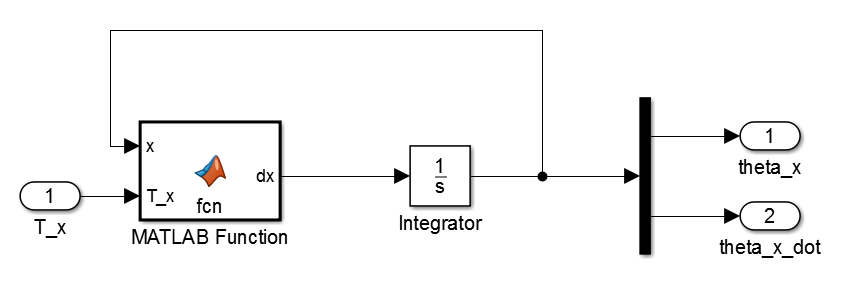
\includegraphics[width=0.45\textwidth]{./Bilder/Florian/Matlab_Funktion_Block.PNG} }}%
	\qquad 
	\subfloat[Aufbau Gesamtsystem inklusive Regler f�r $yz$-Ebene]{{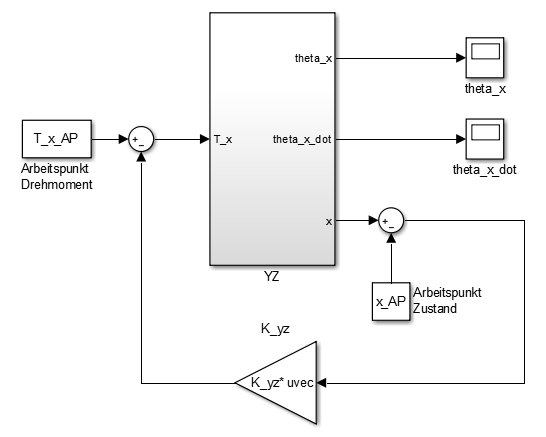
\includegraphics[width=0.45\textwidth]{./Bilder/Florian/Gesamtsystem.PNG} }}%
	\caption{Aufbau Simulinkmodell f�r $yz$-Ebene bestehen aus Subsystem und Gesamtsystem mit Regler}%
	\label{fig:simple_Simulink}%
\end{figure}

Mit der Hinzunahme der Reglerverst�rkungsfaktoren als Zustandsr�ckf�hrung ergibt sich das Gesamtsystem, das in der Abbildung \ref{fig:simple_Simulink} (b) abgebildet ist. Hier ist zu beachten, dass der Zustandsregler f�r das linearisierte Modell ausgelegt wurde. Deshalb muss der Arbeitspunkt des Zustandes vor der R�ckf�hrung abgezogen werden. Nach dem Regler muss der Arbeitspunkt des Drehmomentes analog wieder auf das $\Delta u$ addiert werden. Im Anhang \ref{ch:gesamtbild} ist eine komplette �bersicht des Simulink-Simulationsaufbaus zu sehen.

\subsection{Reale Gegebenheiten}
Die inertiale Messeinheit liefert in der Realit�t verrauschte Signale, die f�r die Berechnung des Regelgesetzes ben�tigt werden. Die St�rke dieses Rauschen kann dem Datenblatt der IMU entnommen werden und in der Simulation durch ein wei�es Rauschen integriert werden. Die Abbildung \ref{fig:Rauschen} zeigt den Einfluss des Rauschen auf den Winkel $\vartheta_{x}$ und das reale Drehmoment $T_{1}$ in der Simulation.  
\begin{figure}[h!]
\centering
% This file was created by matlab2tikz.
%
%The latest updates can be retrieved from
%  http://www.mathworks.com/matlabcentral/fileexchange/22022-matlab2tikz-matlab2tikz
%where you can also make suggestions and rate matlab2tikz.
%
\definecolor{mycolor1}{rgb}{0.00000,0.44700,0.74100}%
%
\begin{tikzpicture}

\begin{axis}[%
width=0.951\figW,
height=0.419\figH,
at={(0\figW,0.581\figH)},
scale only axis,
xmin=0,
xmax=4,
xtick={0,1,2,3,4},
xticklabels={\empty},
ymin=-1,
ymax=1,
ytick={-1,-0.5,0,0.5,1},
yticklabels={{-1},{-0,5},{0},{0,5}},
ylabel style={font=\color{white!15!black}},
ylabel={$\vartheta_{x}$ [$^{\circ}$]},
axis background/.style={fill=white},
xmajorgrids,
ymajorgrids
]
\addplot [color=mycolor1, line width=1.2pt, forget plot]
  table[row sep=crcr]{%
0	0\\
0.0058764	0.0115124409775636\\
0.01087	0.0212888198358809\\
0.021739	0.163762797004292\\
0.032609	0.112179406708664\\
0.043478	0.188354145571307\\
0.05	0.194880134857847\\
0.054348	0.199160129587474\\
0.065217	0.174763586670804\\
0.076087	0.118367350896077\\
0.086957	0.125030850053448\\
0.097826	0.157821224668785\\
0.1	0.160479748838192\\
0.1087	0.171045090580405\\
0.11957	0.199572659199968\\
0.13043	0.227023067164686\\
0.1413	0.216285838083934\\
0.15	0.274057172566975\\
0.15217	0.288472790692467\\
0.16304	0.254616714578187\\
0.17391	0.124652697908662\\
0.18478	0.0291555303630271\\
0.19565	0.134496112829009\\
0.2	0.123077063972052\\
0.20652	0.105974273787397\\
0.21739	0.0458612607956565\\
0.22826	-0.00681304114190062\\
0.23913	-0.0536970316018656\\
0.25	-0.0844998156258938\\
0.26087	-0.115439536562958\\
0.27174	-0.129391058874394\\
0.28261	-0.0411481099729103\\
0.29348	-0.0373769017653593\\
0.3	0.00815605421368727\\
0.30435	0.0385205255244404\\
0.31522	0.0839898831882274\\
0.32609	0.103407422865211\\
0.33696	0.0676090198254371\\
0.34783	0.0393180827752625\\
0.35	0.0363415670295579\\
0.3587	0.0244418065824858\\
0.36957	-0.0515891198735793\\
0.38043	0.0759512853225419\\
0.3913	0.134261200133006\\
0.4	0.101161428308298\\
0.40217	0.0928707290127551\\
0.41304	0.033491101998782\\
0.42391	0.023457465090451\\
0.43478	0.067568912779778\\
0.44565	0.0504936245692892\\
0.45	0.0193396174168458\\
0.45652	-0.0273696209156043\\
0.46739	-0.0826949985712317\\
0.47826	-0.0849409931281445\\
0.48913	-0.015845720782138\\
0.5	-0.0190623058440025\\
0.51087	0.0358132999424472\\
0.52174	0.00436490707486564\\
0.53261	0.00255161024483561\\
0.54348	0.0106524313270723\\
0.55	-0.0482172632492344\\
0.55435	-0.0874390891149149\\
0.56522	-0.223063928800332\\
0.57609	-0.19874759997498\\
0.58696	-0.207072676738231\\
0.59783	-0.136226445370305\\
0.6	-0.136736377807971\\
0.6087	-0.138730270935026\\
0.61957	-0.160926655918394\\
0.63043	-0.191196016235156\\
0.6413	-0.150378502910036\\
0.65	-0.124801666935396\\
0.65217	-0.118401728363785\\
0.66304	-0.0649963322796406\\
0.67391	0.0538901183788247\\
0.68478	0.0919769148523511\\
0.69565	-0.00891980695459666\\
0.7	-0.00523689154327524\\
0.70652	0.00025200402703239\\
0.71739	0.0908997541975051\\
0.72826	0.032150953715971\\
0.73913	0.0313213108286216\\
0.75	-0.057662472501966\\
0.76087	-0.0346874378750152\\
0.77174	-0.0628935771715105\\
0.78261	-0.155202807545037\\
0.79348	-0.120865446882847\\
0.8	-0.0439303930260656\\
0.80435	0.00736021583625056\\
0.81522	0.0467653881963729\\
0.82609	0.0370548994844957\\
0.83696	0.222273247043052\\
0.84783	0.182389654923995\\
0.85	0.195647898303322\\
0.8587	0.248520443637995\\
0.86957	0.2934346051983\\
0.88043	0.33731744272737\\
0.8913	0.340090558455803\\
0.9	0.27342118941438\\
0.90217	0.256713740108365\\
0.91304	0.294374255982314\\
0.92391	0.305065648439455\\
0.93478	0.217706773415859\\
0.94565	0.382334736690798\\
0.95	0.418677449635946\\
0.95652	0.473039685237959\\
0.96739	0.471945335849259\\
0.97826	0.399701087461214\\
0.98913	0.358453855789746\\
1	0.335758997524614\\
1.0109	0.330694050615657\\
1.0217	0.274933797993526\\
1.0326	0.217351539582878\\
1.0435	0.182607378886145\\
1.05	0.147897595657119\\
1.0543	0.124813126091299\\
1.0652	0.190485548569194\\
1.0761	0.132467842234246\\
1.087	0.166461428219358\\
1.0978	0.291876159995544\\
1.1	0.279889882921407\\
1.1087	0.231910397157152\\
1.1196	0.258512827585076\\
1.1304	0.218233894587379\\
1.1413	0.200374800113151\\
1.15	0.132055312621752\\
1.1522	0.114986899904805\\
1.163	0.216767122631844\\
1.1739	0.219311055242225\\
1.1848	0.208464964180399\\
1.1957	0.205869465368456\\
1.2	0.201056619889357\\
1.2065	0.193837351670709\\
1.2174	0.127861261561394\\
1.2283	0.117972010017437\\
1.2391	0.178304465844712\\
1.25	0.303100403202157\\
1.2609	0.30442966528686\\
1.2717	0.156961787976089\\
1.2826	0.23930155271434\\
1.2935	0.228764858861884\\
1.3	0.275529674100462\\
1.3043	0.306681389421724\\
1.3152	0.360780064437977\\
1.3261	0.349229235288139\\
1.337	0.296207720926733\\
1.3478	0.374932121977708\\
1.35	0.364424076015009\\
1.3587	0.322317407650845\\
1.3696	0.280273764644145\\
1.3804	0.335432411581389\\
1.3913	0.354087917390849\\
1.4	0.274710344453425\\
1.4022	0.254863086430093\\
1.413	0.239450521741074\\
1.4239	0.226553241772679\\
1.4348	0.213936711123898\\
1.4457	0.231348898517924\\
1.45	0.19620939694255\\
1.4565	0.143554575570028\\
1.4674	0.113875361782251\\
1.4783	0.0267577019904046\\
1.4891	0.0687377466818449\\
1.5	0.136839510211095\\
1.5109	0.121948337115644\\
1.5217	0.141102316206868\\
1.5326	0.179381626499558\\
1.5435	0.205067324455273\\
1.55	0.22423849228035\\
1.5543	0.236998262377914\\
1.5652	0.221385162460599\\
1.5761	0.242962753025226\\
1.587	0.16331588992409\\
1.5978	0.189408387914348\\
1.6	0.203336991913978\\
1.6087	0.259022760022743\\
1.6196	0.244412336246907\\
1.6304	0.240859997917095\\
1.6413	0.352982108846246\\
1.65	0.339890023227507\\
1.6522	0.336589786327553\\
1.663	0.342571465708719\\
1.6739	0.382695700101731\\
1.6848	0.325371272698892\\
1.6957	0.336796051133801\\
1.7	0.362057760321119\\
1.7065	0.399884433955655\\
1.7174	0.41947959054913\\
1.7283	0.425845151653033\\
1.7391	0.323010686582953\\
1.75	0.24946582399996\\
1.7609	0.120997227175727\\
1.7717	0.0555373720398258\\
1.7826	0.0695570763288819\\
1.7935	0.0605845572571332\\
1.8	0.0229796182893119\\
1.8043	-0.0020015134657305\\
1.8152	0.138260445543019\\
1.8261	0.0990930506678759\\
1.837	0.0995113098583214\\
1.8478	0.0960964813993417\\
1.85	0.0975059575753635\\
1.8587	0.103206887636915\\
1.8696	0.151982784736402\\
1.8804	0.0130703132225243\\
1.8913	-0.0817725365210711\\
1.9	-0.164639422430842\\
1.9022	-0.185294550945308\\
1.913	-0.164032087168003\\
1.9239	-0.166203597211549\\
1.9348	-0.16813446498114\\
1.9457	-0.164713906944209\\
1.95	-0.137910941287989\\
1.9565	-0.0976090899784871\\
1.9674	-0.119920066520881\\
1.9783	-0.217168193088436\\
1.9891	-0.27933411386013\\
2	-0.346650925210051\\
2.0109	-0.425048740317801\\
2.0217	-0.417955522814082\\
2.0326	-0.508362533307774\\
2.0435	-0.520847283663675\\
2.05	-0.469613397623077\\
2.0543	-0.435344791896302\\
2.0652	-0.505056566829869\\
2.0761	-0.522508861269554\\
2.087	-0.57605176722453\\
2.0978	-0.637931209098659\\
2.1	-0.619596559654472\\
2.1087	-0.546028778759675\\
2.1196	-0.578458189964079\\
2.1304	-0.644291040624611\\
2.1413	-0.70542563736507\\
2.15	-0.735162146932359\\
2.1522	-0.742496006710034\\
2.163	-0.721754934526298\\
2.1739	-0.763752740909387\\
2.1848	-0.686747213243805\\
2.1957	-0.69167465028193\\
2.2	-0.680272790158826\\
2.2065	-0.663026760525389\\
2.2174	-0.725536455974162\\
2.2283	-0.744959725229096\\
2.2391	-0.714249187410084\\
2.25	-0.752522768124823\\
2.2609	-0.787759672525369\\
2.2717	-0.781743615676495\\
2.2826	-0.77217522049781\\
2.2935	-0.837549704922237\\
2.3	-0.822710098028349\\
2.3043	-0.812740632393073\\
2.3152	-0.72141115984922\\
2.3261	-0.606819600823055\\
2.337	-0.692304903856574\\
2.3478	-0.585448275064675\\
2.35	-0.563137298522281\\
2.3587	-0.473956417710168\\
2.3696	-0.436421952551148\\
2.3804	-0.474603860018666\\
2.3913	-0.423920013461393\\
2.4	-0.406943273991667\\
2.4022	-0.402743493353358\\
2.413	-0.462749363237409\\
2.4239	-0.474666885376131\\
2.4348	-0.487925128755458\\
2.4457	-0.434628594652389\\
2.45	-0.427581213772279\\
2.4565	-0.417078897387531\\
2.4674	-0.461729498362077\\
2.4783	-0.382094094416843\\
2.4891	-0.3013185044593\\
2.5	-0.285877291880524\\
2.5109	-0.242315310716728\\
2.5217	-0.212779336377734\\
2.5326	-0.198501228123074\\
2.5435	-0.294104965818603\\
2.55	-0.247512037918564\\
2.5543	-0.216503562046084\\
2.5652	-0.27017824829394\\
2.5761	-0.279849775875748\\
2.587	-0.230947828061332\\
2.5978	-0.150951460705167\\
2.6	-0.167011467702684\\
2.6087	-0.23137754640768\\
2.6196	-0.249620522604646\\
2.6304	-0.329720022363935\\
2.6413	-0.24872097886629\\
2.65	-0.254559418798673\\
2.6522	-0.25603192033216\\
2.663	-0.289939562648002\\
2.6739	-0.413520829479769\\
2.6848	-0.485799455335522\\
2.6957	-0.512436263231154\\
2.7	-0.47269591056088\\
2.7065	-0.413005167464151\\
2.7174	-0.413767201331675\\
2.7283	-0.426458216493823\\
2.7391	-0.406536473957124\\
2.75	-0.408438693836959\\
2.7609	-0.393014669992037\\
2.7717	-0.345808677251208\\
2.7826	-0.334716214337476\\
2.7935	-0.288146204749242\\
2.8	-0.289085855533257\\
2.8043	-0.289739027419706\\
2.8152	-0.31778531149136\\
2.8261	-0.246394770218059\\
2.837	-0.219969956706626\\
2.8478	-0.262724067379288\\
2.85	-0.271868473789576\\
2.8587	-0.308486206476387\\
2.8696	-0.188548951221651\\
2.8804	-0.16217570391178\\
2.8913	-0.302750898947127\\
2.9	-0.312325023703763\\
2.9022	-0.314714257709459\\
2.913	-0.246566657556598\\
2.9239	-0.218520373484945\\
2.9348	-0.251253452320769\\
2.9457	-0.232145309853156\\
2.95	-0.281866587314609\\
2.9565	-0.356437044350885\\
2.9674	-0.308085136019795\\
2.9783	-0.243323716436158\\
2.9891	-0.277219899596098\\
3	-0.25677676546583\\
3.0109	-0.151157725511414\\
3.0217	-0.173462972475857\\
3.0326	-0.124939176806227\\
3.0435	-0.115422347829104\\
3.05	-0.105361208946607\\
3.0543	-0.0987034393671869\\
3.0652	0.0637186363964989\\
3.0761	0.154480880723173\\
3.087	0.107945248602647\\
3.0978	0.0482906018470112\\
3.1	0.0322088224532792\\
3.1087	-0.0322300218916991\\
3.1196	-0.00192450793806492\\
3.1304	0.0982679914428875\\
3.1413	0.0610715713829945\\
3.15	0.0424928419180824\\
3.1522	0.0378255277189467\\
3.163	0.0899543738355393\\
3.1739	0.131992287264288\\
3.1848	0.187912968069056\\
3.1957	0.225017714881728\\
3.2	0.222760261168913\\
3.2065	0.219248029884761\\
3.2174	0.197246450551737\\
3.2283	0.16152253202533\\
3.2391	0.161029788321518\\
3.25	0.11154915313402\\
3.2609	0.112998736355701\\
3.2717	0.0767935332813842\\
3.2826	0.0143457172744856\\
3.2935	0.0342995454477116\\
3.3	0.0635811265256675\\
3.3043	0.0831132577616772\\
3.3152	0.220955444114251\\
3.3261	0.288604570985347\\
3.337	0.209977572759544\\
3.3478	0.249001728185904\\
3.35	0.225378678292661\\
3.3587	0.130829182940172\\
3.3696	0.115307756270078\\
3.3804	0.106489935803015\\
3.3913	0.116705773290197\\
3.4	0.144591629179215\\
3.4022	0.151564525545957\\
3.413	0.185775835493218\\
3.4239	0.165980143671448\\
3.4348	0.205468394911865\\
3.4457	0.197441256202082\\
3.45	0.182865209893954\\
3.4565	0.160978222119956\\
3.4674	0.147359015329696\\
3.4783	0.0322569509080702\\
3.4891	0.0782259277692113\\
3.5	0.0788619109218065\\
3.5109	0.152509905907923\\
3.5217	0.144144722099013\\
3.5326	-0.00730635780350826\\
3.5435	0.0453622145560975\\
3.55	0.0434645783386243\\
3.5543	0.0422287083745271\\
3.5652	0.125042309209351\\
3.5761	0.148625252056936\\
3.587	0.0775154601032491\\
3.5978	0.013856984275239\\
3.6	0.0185884697474293\\
3.6087	0.0375791558670404\\
3.6196	0.0889287793822551\\
3.6304	0.0804891110599781\\
3.6413	0.0713504342276414\\
3.65	0.0612377291435824\\
3.6522	0.0587167148450068\\
3.663	0.00639592786704538\\
3.6739	0.0708003947443158\\
3.6848	0.03994203381416\\
3.6957	-0.0106243563951109\\
3.7	-0.0386127717294564\\
3.7065	-0.0805234885276859\\
3.7174	-0.0178928989841405\\
3.7283	-0.0498066481729273\\
3.7391	-0.0934035797622268\\
3.75	-0.118711125573155\\
3.7609	-0.170162735575903\\
3.7717	-0.189379740024591\\
3.7826	-0.219563156672083\\
3.7935	-0.256169430202991\\
3.8	-0.265119030962934\\
3.8043	-0.270997577940977\\
3.8152	-0.220308001805753\\
3.8261	-0.329628349116714\\
3.837	-0.323262788012811\\
3.8478	-0.401924163706321\\
3.85	-0.444328770123953\\
3.8587	-0.613637798585112\\
3.8696	-0.624523996692597\\
3.8804	-0.57530692209086\\
3.8913	-0.513226944988435\\
3.9	-0.46814089608959\\
3.9022	-0.456830709213708\\
3.913	-0.430549135151057\\
3.9239	-0.500306746708235\\
3.9348	-0.431145011257993\\
3.9457	-0.491987399522935\\
3.95	-0.496078318180169\\
3.9565	-0.502134482074702\\
3.9674	-0.495499630807087\\
3.9783	-0.552652170871387\\
3.9891	-0.571978037301149\\
4	-0.631857856470272\\
4.0109	-0.496937754872866\\
4.0217	-0.551305720052829\\
4.0326	-0.550623900276624\\
4.0435	-0.572654127499404\\
4.05	-0.582640781868534\\
4.0543	-0.589229796512539\\
4.0652	-0.600803543974181\\
4.0761	-0.580005176010932\\
4.087	-0.518755987711447\\
4.0978	-0.632258926926863\\
4.1	-0.628248222360948\\
4.1087	-0.612148108317772\\
4.1196	-0.588026585142764\\
4.1304	-0.616502587560766\\
4.1413	-0.733271386208428\\
4.15	-0.631055715557089\\
4.1522	-0.605501797894254\\
4.163	-0.631399490234167\\
4.1739	-0.573301569807902\\
4.1848	-0.570133113200828\\
4.1957	-0.513221215410484\\
4.2	-0.517329322801572\\
4.2065	-0.523528726144887\\
4.2174	-0.519735745541121\\
4.2283	-0.489815889479389\\
4.2391	-0.456716117654682\\
4.25	-0.407602175456068\\
4.2609	-0.445039237789916\\
4.2717	-0.403877949787717\\
4.2826	-0.409693471408295\\
4.2935	-0.501234938336347\\
4.3	-0.498221180333959\\
4.3043	-0.496210098473049\\
4.3152	-0.434760374945269\\
4.3261	-0.38597874826783\\
4.337	-0.351721601696958\\
4.3478	-0.310027462945288\\
4.35	-0.30683608802641\\
4.3587	-0.294213827799678\\
4.3696	-0.209668175550173\\
4.3804	-0.123151548485419\\
4.3913	-0.150166508525837\\
4.4	-0.179032122244528\\
4.4022	-0.186291497508836\\
4.413	-0.207009651380766\\
4.4239	-0.228168982754948\\
4.4348	-0.310119136192509\\
4.4457	-0.314553829526822\\
4.45	-0.305180239998482\\
4.4565	-0.291119855705971\\
4.4674	-0.27701363478985\\
4.4783	-0.176660076972687\\
4.4891	-0.169091304499009\\
4.5	-0.161854847546506\\
4.5109	-0.141050750005306\\
4.5217	-0.181570325276958\\
4.5326	-0.144328068593454\\
4.5435	-0.0535778563804784\\
4.55	-0.0167395349425421\\
4.5543	0.00773263840308559\\
4.5652	0.0890032638956221\\
4.5761	0.0944177150596084\\
4.587	0.0228329410937584\\
4.5978	-0.0831247169175798\\
4.6	-0.0772862769851967\\
4.6087	-0.0539548626096745\\
4.6196	-0.0152040080515915\\
4.6304	-0.0398675493007929\\
4.6413	-0.0271392918819617\\
4.65	-0.0738428006364605\\
4.6522	-0.0855196805012267\\
4.663	-0.117427700112062\\
4.6739	-0.0360103974239722\\
4.6848	0.0101132780418542\\
4.6957	-0.0498719653615722\\
4.7	-0.0431477326779169\\
4.7065	-0.0330814371752635\\
4.7174	-0.161190216504154\\
4.7283	-0.142041966990882\\
4.7391	-0.116430753548535\\
4.75	-0.177192927722158\\
4.7609	-0.276452136150622\\
4.7717	-0.205772062543284\\
4.7826	-0.11286122648487\\
4.7935	-0.119364297459604\\
4.8	-0.137641651124278\\
4.8043	-0.149817004270808\\
4.8152	-0.226060498068866\\
4.8261	-0.1946738700516\\
4.837	-0.213913792812093\\
4.8478	-0.296093129367707\\
4.85	-0.301026295983783\\
4.8587	-0.32063291173316\\
4.8696	-0.275483837476851\\
4.8804	-0.28704039620464\\
4.8913	-0.269966253909741\\
4.9	-0.306555338706796\\
4.9022	-0.31568255638323\\
4.913	-0.338297200557043\\
4.9239	-0.280371167469317\\
4.9348	-0.281442598546212\\
4.9457	-0.238923400569553\\
4.95	-0.220966903270153\\
4.9565	-0.194049346054907\\
4.9674	-0.184801807241496\\
4.9783	-0.130330709658408\\
4.9891	-0.100789005741463\\
5	-0.15609089212749\\
5.0109	-0.0858691847562565\\
5.0217	-0.118361621318125\\
5.0326	-0.234339738208507\\
5.0435	-0.190812134512418\\
5.05	-0.216085302855639\\
5.0543	-0.232918802876582\\
5.0652	-0.135619110107466\\
5.0761	-0.219196463683199\\
5.087	-0.331255549254885\\
5.0978	-0.373534104957589\\
5.1	-0.380518460480234\\
5.1087	-0.408318372699981\\
5.1196	-0.401735087633928\\
5.1304	-0.347911432359338\\
5.1413	-0.28660494828034\\
5.15	-0.327359436247996\\
5.1522	-0.337535166689519\\
5.163	-0.342330823434764\\
5.1739	-0.381733131005911\\
5.1848	-0.319091655264258\\
5.1957	-0.243587277021918\\
5.2	-0.2301514167261\\
5.2065	-0.210040598117009\\
5.2174	-0.296540036447909\\
5.2283	-0.303077484890352\\
5.2391	-0.240544871129774\\
5.25	-0.229589918086872\\
5.2609	-0.229165929318475\\
5.2717	-0.216371781753204\\
5.2826	-0.134398710003837\\
5.2935	-0.115382240783445\\
5.3	-0.165521777435344\\
5.3043	-0.198988242248935\\
5.3152	-0.301221101634128\\
5.3261	-0.312342212437617\\
5.337	-0.249036105653612\\
5.3478	-0.213489804043696\\
5.35	-0.211673527833131\\
5.3587	-0.204425611724726\\
5.3696	-0.257664850048283\\
5.3804	-0.216102491589493\\
5.3913	-0.248497525326189\\
5.4	-0.290678678203721\\
5.4022	-0.301209642478225\\
5.413	-0.30193156930009\\
5.4239	-0.337993532925624\\
5.4348	-0.349234964866091\\
5.4457	-0.269158383418607\\
5.45	-0.286960182113321\\
5.4565	-0.313654285788467\\
5.4674	-0.396652951991118\\
5.4783	-0.438072071001125\\
5.4891	-0.424246599404618\\
5.5	-0.302693603167614\\
5.5109	-0.256358506275384\\
5.5217	-0.253671334216221\\
5.5326	-0.219700666542914\\
5.5435	-0.165126436556703\\
5.55	-0.144740598205949\\
5.5543	-0.131207335084959\\
5.5652	-0.179118065913798\\
5.5761	-0.0728802315406407\\
5.587	-0.135842563647567\\
5.5978	-0.136839510211095\\
5.6	-0.152693252402364\\
5.6087	-0.216154057791054\\
5.6196	-0.19108142467613\\
5.6304	-0.199177318321328\\
5.6413	-0.211925629262989\\
5.65	-0.157975923273471\\
5.6522	-0.144499955931994\\
5.663	-0.199051267606399\\
5.6739	-0.0839555057205195\\
5.6848	-0.0255436044225224\\
5.6957	-0.015433764127439\\
5.7	-0.0292890295292926\\
5.7065	-0.0501572983435474\\
5.7174	0.00530891233812318\\
5.7283	0.0269467780627977\\
5.7391	0.017330254429322\\
5.75	0.107326454183906\\
5.7609	0.171698262466854\\
5.7717	0.144075967163597\\
5.7826	0.226008931867305\\
5.7935	0.201979081939518\\
5.8	0.141509116241411\\
5.8043	0.101132780418542\\
5.8152	0.0762377642201073\\
5.8261	0.0955464419160161\\
5.837	0.0914440641028794\\
5.8478	0.0411429533527542\\
5.85	0.0214354970314344\\
5.8587	-0.0573588048705467\\
5.8696	-0.0257790900763211\\
5.8804	-0.0437779862525608\\
5.8913	-0.0615413967750017\\
5.9	-0.138174501873749\\
5.9022	-0.157305562653168\\
5.913	-0.0959933489962181\\
5.9239	-0.108162972564797\\
5.9348	-0.0294059129194992\\
5.9457	-0.0855368692350806\\
5.95	-0.0633404842517125\\
5.9565	-0.0300252802960357\\
5.9674	-0.0815261646691648\\
5.9783	-0.197744923833501\\
5.9891	-0.210023409383155\\
6	-0.221763314605385\\
6.0109	-0.190073018956699\\
6.0217	-0.177021040383619\\
6.0326	-0.104708037060158\\
6.0435	-0.0975804420887305\\
6.05	-0.100794735319414\\
6.0543	-0.102943327051155\\
6.0652	-0.211071922148244\\
6.0761	-0.244360770045345\\
6.087	-0.240676651422654\\
6.0978	-0.224003579584347\\
6.1	-0.241937158571941\\
6.1087	-0.313585530853051\\
6.1196	-0.247259936488707\\
6.1304	-0.193722760111683\\
6.1413	-0.259183188205379\\
6.15	-0.351652846761543\\
6.1522	-0.374737316327364\\
6.163	-0.346421742091998\\
6.1739	-0.345843054718916\\
6.1848	-0.347223883005181\\
6.1957	-0.425759207983763\\
6.2	-0.372307975276009\\
6.2065	-0.292070965645888\\
6.2174	-0.332985881796181\\
6.2283	-0.32361229226784\\
6.2391	-0.372697586576698\\
6.25	-0.506786899371164\\
6.2609	-0.541267499482137\\
6.2717	-0.509313643247691\\
6.2826	-0.557092593783651\\
6.2935	-0.586536894875424\\
6.3	-0.592495655944784\\
6.3043	-0.596391768951674\\
6.3152	-0.537583380859446\\
6.3261	-0.511181485659818\\
6.337	-0.462119109662765\\
6.3478	-0.415377212735993\\
6.35	-0.420493725846511\\
6.3587	-0.440959778288584\\
6.3696	-0.341477116320019\\
6.3804	-0.292987698118098\\
6.3913	-0.382426409938019\\
6.4	-0.336469465190576\\
6.4022	-0.324993120554106\\
6.413	-0.394000157399662\\
6.4239	-0.318999982017037\\
6.4348	-0.301009107249929\\
6.4457	-0.280978502732156\\
6.45	-0.264408563296972\\
6.4565	-0.239622409079613\\
6.4674	-0.170901851131622\\
6.4783	-0.18841144135082\\
6.4891	-0.230987935106991\\
6.5	-0.144459848886334\\
6.5109	-0.0952485038625481\\
6.5217	-0.200174264884856\\
6.5326	-0.194565008070525\\
6.5435	-0.197985566107456\\
6.55	-0.229681591334093\\
6.5543	-0.25082373397442\\
6.5652	-0.283505246608683\\
6.5761	-0.236390927115075\\
6.587	-0.102496419970953\\
6.5978	-0.0336509572236235\\
6.6	-0.0400445932594884\\
6.6087	-0.0657755548810185\\
6.6196	-0.0760143106800063\\
6.6304	-0.0918680528712762\\
6.6413	-0.0868031059623197\\
6.65	-0.0925785205372384\\
6.6522	-0.094039562914822\\
6.663	-0.129104579976828\\
6.6739	-0.140506440099932\\
6.6848	-0.172895744258677\\
6.6957	-0.0931457487544179\\
6.7	-0.0772920065631481\\
6.7065	-0.0535549380686732\\
6.7174	-0.00411504018040909\\
6.7283	-0.00977294111154645\\
6.7391	-0.0252330612975615\\
6.75	0.0185638325622387\\
6.7609	-0.0615070193072939\\
6.7717	0.0478053065945354\\
6.7826	0.126675238925474\\
6.7935	0.235153338277592\\
6.8	0.24044173872665\\
6.8043	0.24385656718563\\
6.8152	0.289985399271612\\
6.8261	0.197401149156423\\
6.837	0.125065227521156\\
6.8478	0.117651153652163\\
6.85	0.104226752512248\\
6.8587	0.0505142510499139\\
6.8696	0.0155517934332359\\
6.8804	0.0258140405018241\\
6.8913	0.0259171729049477\\
6.9	0.00677236113844633\\
6.9022	0.0019949244510865\\
6.913	-0.116774528225613\\
6.9239	-0.151415556519223\\
6.9348	-0.225080740239193\\
6.9457	-0.223419162633313\\
6.95	-0.242647626237904\\
6.9565	-0.271347082196007\\
6.9674	-0.210963060167169\\
6.9783	-0.217277055069511\\
6.9891	-0.181106229462902\\
7	-0.172752504809895\\
7.0109	-0.141698192313804\\
7.0217	-0.224416109196841\\
7.0326	-0.188090584985547\\
7.0435	-0.209318671295144\\
7.05	-0.254989137145022\\
7.0543	-0.285384548176712\\
7.0652	-0.268493752376255\\
7.0761	-0.342875133340139\\
7.087	-0.269387566536659\\
7.0978	-0.336160067981205\\
7.1	-0.327571430632194\\
7.1087	-0.293102289677124\\
7.1196	-0.2132892688154\\
7.1304	-0.177846099608608\\
7.1413	-0.285373089020809\\
7.15	-0.322449187943725\\
7.1522	-0.331702456335087\\
7.163	-0.253911976490176\\
7.1739	-0.217076519841215\\
7.1848	-0.128084715101496\\
7.1957	-0.0867916468064171\\
7.2	-0.0615815038206609\\
7.2065	-0.0238665569561744\\
7.2174	0.0171474808926753\\
7.2283	-0.00255562094940152\\
7.2391	0.0307678335985252\\
7.25	0.0497751354941951\\
7.2609	0.147697060428824\\
7.2717	0.20050085082808\\
7.2826	0.137538518721154\\
7.2935	0.212601719461243\\
7.3	0.218606317154214\\
7.3043	0.222513889317007\\
7.3152	0.242756488218978\\
7.3261	0.249981486015578\\
7.337	0.297485416809875\\
7.3478	0.329255926549879\\
7.35	0.319343756694116\\
7.3587	0.279523189932523\\
7.3696	0.206522637254905\\
7.3804	0.200357611379298\\
7.3913	0.266522777561005\\
7.4	0.330396112562189\\
7.4022	0.346330068844777\\
7.413	0.332441571890806\\
7.4239	0.342187583985982\\
7.4348	0.398039509855334\\
7.4457	0.381670105648447\\
7.45	0.376542133382026\\
7.4565	0.368749907368246\\
7.4674	0.370571913156763\\
7.4783	0.360986329244224\\
7.4891	0.358597095238528\\
7.5	0.398664033852027\\
7.5109	0.394206422205909\\
7.5217	0.41615070575942\\
7.5326	0.451960567955096\\
7.5435	0.308497665632289\\
7.55	0.307781468388376\\
7.5543	0.30731737257432\\
7.5652	0.321887689304496\\
7.5761	0.439859699321933\\
7.587	0.470025927235571\\
7.5978	0.43130543944063\\
7.6	0.416488750858547\\
7.6087	0.357187619062507\\
7.6196	0.439899806367592\\
7.6304	0.425650346002689\\
7.6413	0.287080503250299\\
7.65	0.305397963960631\\
7.6522	0.309993085477581\\
7.663	0.274807747278597\\
7.6739	0.359594041802056\\
7.6848	0.357485557115975\\
7.6957	0.316118004307529\\
7.7	0.27004646800106\\
7.7065	0.200987864953941\\
7.7174	0.178550837696618\\
7.7283	0.0840471789677405\\
7.7391	-0.0149249776053628\\
7.75	0.0686059663889648\\
7.7609	0.0632258926926863\\
7.7717	0.00761632797067403\\
7.7826	0.0242263744515166\\
7.7935	0.0101167157886249\\
7.8	0.0456807790901903\\
7.8043	0.0694424847698558\\
7.8152	-0.0547925269061558\\
7.8261	-0.0107229051358734\\
7.837	0.0354855680836324\\
7.8478	0.042661864467646\\
7.85	0.0403047160984778\\
7.8587	0.0309339913591131\\
7.8696	-0.0112895603952577\\
7.8804	-0.0328018337712396\\
7.8913	-8.07698603795922e-05\\
7.9	-0.0108317671169482\\
7.9022	-0.0135034693156432\\
7.913	-0.0717343159503791\\
7.9239	-0.0990071069986063\\
7.9348	-0.0666922873532278\\
7.9457	-0.0295239422252962\\
7.95	-0.0616559883340279\\
7.9565	-0.109807361436822\\
7.9674	-0.126778371328597\\
7.9783	-0.112632043366817\\
7.9891	-0.09175346131225\\
8	-0.113543046261075\\
8.0109	-0.0239530735832392\\
8.0217	-0.0558748441811579\\
8.0326	-0.0726109413769292\\
8.0435	-0.0600803543974181\\
8.05	-0.0366876335378169\\
8.0543	-0.0210945871433315\\
8.0652	-0.0487071421640713\\
8.0761	-0.0325468675524064\\
8.087	-0.0859322101137209\\
8.0978	-0.0804203561245624\\
8.1	-0.0673110817719691\\
8.1087	-0.0148510660497909\\
8.1196	0.0303753575088606\\
8.1304	0.0371975659754833\\
8.1413	0.175966798040578\\
8.15	0.161035517899469\\
8.1522	0.157259726029557\\
8.163	0.111646555959192\\
8.1739	0.122463999131262\\
8.1848	0.0899371851016853\\
8.1957	0.0709321750371959\\
8.2	0.0909685091329208\\
8.2065	0.120980038441873\\
8.2174	0.00593928050432611\\
8.2283	0.0682965691795941\\
8.2391	-0.117141221214497\\
8.25	-0.156342993557348\\
8.2609	-0.0527568078600559\\
8.2717	-0.0577484161712357\\
8.2826	-0.105613310376465\\
8.2935	-0.0536603623029773\\
8.3	-0.0412947871684638\\
8.3043	-0.0330396112562189\\
8.3152	-0.0230856154814111\\
8.3261	-0.00750574711621379\\
8.337	0.0143107668489826\\
8.3478	0.0955063348703569\\
8.35	0.100937974768197\\
8.3587	0.122549942800532\\
8.3696	0.346026401213358\\
8.3804	0.390505114849364\\
8.3913	0.474071009269194\\
8.4	0.419565534218399\\
8.4022	0.405871842914773\\
8.413	0.415062085948671\\
8.4239	0.390917644461858\\
8.4348	0.393163639018771\\
8.4457	0.355675010483361\\
8.45	0.334194822743907\\
8.4565	0.301908650988285\\
8.4674	0.378805316672792\\
8.4783	0.449640088884816\\
8.4891	0.451404798893819\\
8.5	0.458956382633643\\
8.5109	0.50475289919845\\
8.5217	0.537692242840521\\
8.5326	0.501681845416549\\
8.5435	0.352460717252677\\
8.55	0.339804079558237\\
8.5543	0.331375870391863\\
8.5652	0.246280178659033\\
8.5761	0.204723549778194\\
8.587	0.433419653704663\\
8.5978	0.369689558152261\\
8.6	0.35185911156779\\
8.6087	0.280543054807856\\
8.6196	0.27595939244681\\
8.6304	0.157660796486149\\
8.6413	0.0963199349394427\\
8.65	0.112763823659697\\
8.6522	0.116912038096444\\
8.663	0.132336061941366\\
8.6739	0.18052754208982\\
8.6848	0.0683825128488638\\
8.6957	0.153781872213113\\
8.7	0.167756312836354\\
8.7065	0.18876094560585\\
8.7174	0.312983925168163\\
8.7283	0.263761120988474\\
8.7391	0.220760638463906\\
8.75	0.138839132916101\\
8.7609	0.139045397722348\\
8.7717	0.00802943054096336\\
8.7826	0.0382294629645139\\
8.7935	0.0127202360096994\\
8.8	0.00209387426230559\\
8.8043	-0.00492119179815815\\
8.8152	-0.00475056496676819\\
8.8261	0.035413948359241\\
8.837	-0.0684398086283768\\
8.8478	-0.0516848038253662\\
8.85	-0.0496021022400656\\
8.8587	-0.0411544125086568\\
8.8696	-0.0798875053750907\\
8.8804	-0.0977867068949776\\
8.8913	-0.175451136024961\\
8.9	-0.166547371888628\\
8.9022	-0.164284188597861\\
8.913	-0.224387461307084\\
8.9239	-0.233056312747414\\
8.9348	-0.300155400135184\\
8.9457	-0.302424313003902\\
8.95	-0.337477870910006\\
8.9565	-0.389897779586525\\
8.9674	-0.40866214737706\\
8.9783	-0.335976721486763\\
8.9891	-0.301089321341248\\
9	-0.27201744281631\\
9.0109	-0.285957505971843\\
9.0217	-0.209524936101391\\
9.0326	-0.14575473350333\\
9.0435	-0.0696544791540542\\
9.05	-0.0727026146241502\\
9.0543	-0.0747824514204751\\
9.0652	-0.023286723667502\\
9.0761	0.0645150477317307\\
9.087	0.0536362980755818\\
9.0978	0.0131407870313254\\
9.1	0.0268768772117918\\
9.1087	0.0816923224297528\\
9.1196	0.114305080128599\\
9.1304	0.130983881544858\\
9.1413	0.0615528559309043\\
9.15	0.0482149714180539\\
9.1522	0.0448625953587435\\
9.163	0.105166403296263\\
9.1739	0.0802541983639744\\
9.1848	0.099001377420655\\
9.1957	0.10611751323618\\
9.2	0.125844450122534\\
9.2065	0.155357506149723\\
9.2174	0.0825689478563029\\
9.2283	0.143073291022118\\
9.2391	0.165378537986561\\
9.25	0.169503834111503\\
9.2609	0.179192550427165\\
9.2717	0.118493401611006\\
9.2826	0.110884522091668\\
9.2935	0.0744042992756887\\
9.3	0.0909398612431643\\
9.3043	0.10195783964353\\
9.3152	0.0734360006019176\\
9.3261	0.14951906621734\\
9.337	0.164140949149078\\
9.3478	0.170265867979027\\
9.35	0.160210458674481\\
9.3587	0.119948714410638\\
9.3696	0.196707870224314\\
9.3804	0.26409343650965\\
9.3913	0.259549881194263\\
9.4	0.275483837476851\\
9.4022	0.279442975841205\\
9.413	0.410163296800302\\
9.4239	0.401809572147295\\
9.4348	0.371070386438526\\
9.4457	0.343327769998292\\
9.45	0.382185767664064\\
9.4565	0.440381090915502\\
9.4674	0.447726409849079\\
9.4783	0.458297481169243\\
9.4891	0.478351003998822\\
9.5	0.496313230876173\\
9.5109	0.376777046078029\\
9.5217	0.280755049192055\\
9.5326	0.256129323157332\\
9.5435	0.269043791859581\\
9.55	0.252479582002349\\
9.5543	0.241467333179934\\
9.5652	0.187763999042322\\
9.5761	0.0862244185892376\\
9.587	0.0946812756453685\\
9.5978	0.236287794711951\\
9.6	0.235978397502581\\
9.6087	0.234752267821001\\
9.6196	0.148648170368741\\
9.6304	0.137968237067502\\
9.6413	0.122842151276049\\
9.65	0.136020180564057\\
9.6522	0.139337606197865\\
9.663	0.209335860028998\\
9.6739	0.21398827732546\\
9.6848	0.239101017486044\\
9.6957	0.223952013382785\\
9.7	0.210252592501207\\
9.7065	0.189712055545767\\
9.7174	0.138449521615412\\
9.7283	0.222765990746864\\
9.7391	0.275317679716263\\
9.75	0.228105957397483\\
9.7609	0.149490418327583\\
9.7717	0.246182775833861\\
9.7826	0.161224593971862\\
9.7935	0.140558006301494\\
9.8	0.12626270931298\\
9.8043	0.11676306906971\\
9.8152	0.151902570645084\\
9.8261	0.201532174859316\\
9.837	0.233314143755223\\
9.8478	0.168564183327488\\
9.85	0.176339220607413\\
9.8587	0.207445099305066\\
9.8696	0.152349477725286\\
9.8804	0.141543493709119\\
9.8913	0.223344678119946\\
9.9	0.247483390028808\\
9.9022	0.253505176455633\\
9.913	0.184125717043241\\
9.9239	0.210315617858671\\
9.9348	0.244658708098813\\
9.9457	0.183930911392897\\
9.95	0.178608133476132\\
9.9565	0.170644020123813\\
9.9674	0.219454294691008\\
9.9783	0.283677133947222\\
9.9891	0.262116732116449\\
10	0.309912871386262\\
};
\end{axis}

\begin{axis}[%
width=0.951\figW,
height=0.419\figH,
at={(0\figW,0\figH)},
scale only axis,
xmin=0,
xmax=4,
xtick={0,1,2,3,4},
xlabel style={font=\color{white!15!black}},
xlabel={t [$s$]},
ymin=-0.1,
ymax=0.1,
ytick={-0.1,-0.05,0,0.05,0.1},
yticklabels={{-0,1},{-0,05},{0},{0,05},{0,1}},
ylabel style={font=\color{white!15!black}},
ylabel={$T_{1}$ [$Nm$]},
axis background/.style={fill=white},
xmajorgrids,
ymajorgrids
]
\addplot [color=red, line width=1.2pt, forget plot]
  table[row sep=crcr]{%
0	0\\
0.0058764	0.00062495\\
0.01087	0.0011412\\
0.021739	0.0087183\\
0.032609	0.005499\\
0.043478	0.0093197\\
0.05	0.0093976\\
0.054348	0.0094492\\
0.065217	0.0077079\\
0.076087	0.0043644\\
0.086957	0.0045927\\
0.097826	0.0062163\\
0.1	0.0063176\\
0.1087	0.0067128\\
0.11957	0.008014\\
0.13043	0.0092008\\
0.1413	0.008293\\
0.15	0.01119\\
0.15217	0.011894\\
0.16304	0.0096363\\
0.17391	0.0023672\\
0.18478	-0.0026573\\
0.19565	0.0033424\\
0.2	0.0027288\\
0.20652	0.001834\\
0.21739	-0.0012895\\
0.22826	-0.0038555\\
0.23913	-0.0059896\\
0.25	-0.0071689\\
0.26087	-0.0083174\\
0.27174	-0.0085209\\
0.28261	-0.0032634\\
0.29348	-0.0028365\\
0.3	-0.0002517\\
0.30435	0.001423\\
0.31522	0.003818\\
0.32609	0.0046932\\
0.33696	0.0025713\\
0.34783	0.00097305\\
0.35	0.00081126\\
0.3587	0.00018204\\
0.36957	-0.0038459\\
0.38043	0.0032473\\
0.3913	0.0062441\\
0.4	0.0042342\\
0.40217	0.0037461\\
0.41304	0.00042902\\
0.42391	-6.2099e-05\\
0.43478	0.0023726\\
0.44565	0.001396\\
0.45	-0.00030463\\
0.45652	-0.0027846\\
0.46739	-0.0055375\\
0.47826	-0.0053112\\
0.48913	-0.0012904\\
0.5	-0.0013728\\
0.51087	0.0016586\\
0.52174	-0.00010097\\
0.53261	-0.00017591\\
0.54348	0.00028339\\
0.55	-0.0029072\\
0.55435	-0.0049751\\
0.56522	-0.011969\\
0.57609	-0.010037\\
0.58696	-0.009988\\
0.59783	-0.0057224\\
0.6	-0.0057046\\
0.6087	-0.0056365\\
0.61957	-0.0066219\\
0.63043	-0.0079985\\
0.6413	-0.0055046\\
0.65	-0.0039974\\
0.65217	-0.0036313\\
0.66304	-0.0007154\\
0.67391	0.0055545\\
0.68478	0.0071695\\
0.69565	0.0012715\\
0.7	0.0014081\\
0.70652	0.0016078\\
0.71739	0.0063017\\
0.72826	0.0027495\\
0.73913	0.0025088\\
0.75	-0.0024347\\
0.76087	-0.0011087\\
0.77174	-0.0026004\\
0.78261	-0.0074512\\
0.79348	-0.0052635\\
0.8	-0.00096249\\
0.80435	0.0018244\\
0.81522	0.0037685\\
0.82609	0.0029864\\
0.83696	0.012707\\
0.84783	0.0098625\\
0.85	0.01048\\
0.8587	0.012885\\
0.86957	0.014639\\
0.88043	0.016278\\
0.8913	0.015664\\
0.9	0.011511\\
0.90217	0.010503\\
0.91304	0.012136\\
0.92391	0.012257\\
0.93478	0.007138\\
0.94565	0.015818\\
0.95	0.017553\\
0.95652	0.020087\\
0.96739	0.019241\\
0.97826	0.014666\\
0.98913	0.012028\\
1	0.010544\\
1.0109	0.010097\\
1.0217	0.0069645\\
1.0326	0.0039062\\
1.0435	0.002231\\
1.05	0.00051302\\
1.0543	-0.00060113\\
1.0652	0.0033199\\
1.0761	0.00038498\\
1.087	0.002527\\
1.0978	0.0094411\\
1.1	0.0087464\\
1.1087	0.0060455\\
1.1196	0.0074779\\
1.1304	0.0052494\\
1.1413	0.0043436\\
1.15	0.00073881\\
1.1522	-0.00013739\\
1.163	0.0056446\\
1.1739	0.0057875\\
1.1848	0.0052048\\
1.1957	0.005095\\
1.2	0.0048463\\
1.2065	0.0044835\\
1.2174	0.0010108\\
1.2283	0.00072371\\
1.2391	0.0042036\\
1.25	0.010944\\
1.2609	0.010709\\
1.2717	0.0025268\\
1.2826	0.0071061\\
1.2935	0.0064582\\
1.3	0.0089651\\
1.3043	0.01059\\
1.3152	0.01323\\
1.3261	0.012227\\
1.337	0.0090717\\
1.3478	0.01316\\
1.35	0.012514\\
1.3587	0.010001\\
1.3696	0.0075909\\
1.3804	0.010526\\
1.3913	0.011351\\
1.4	0.0069037\\
1.4022	0.0058231\\
1.413	0.0050885\\
1.4239	0.0045227\\
1.4348	0.0039951\\
1.4457	0.0050973\\
1.45	0.0032247\\
1.4565	0.00049366\\
1.4674	-0.0007584\\
1.4783	-0.0050407\\
1.4891	-0.0021978\\
1.5	0.0018659\\
1.5109	0.0012466\\
1.5217	0.0024759\\
1.5326	0.0046557\\
1.5435	0.0060395\\
1.55	0.0070379\\
1.5543	0.0076852\\
1.5652	0.0066991\\
1.5761	0.0077662\\
1.587	0.0033554\\
1.5978	0.0048516\\
1.6	0.0056178\\
1.6087	0.0085971\\
1.6196	0.0076306\\
1.6304	0.0073169\\
1.6413	0.013226\\
1.65	0.012193\\
1.6522	0.011942\\
1.663	0.011945\\
1.6739	0.013794\\
1.6848	0.010338\\
1.6957	0.010768\\
1.7	0.012064\\
1.7065	0.013954\\
1.7174	0.014651\\
1.7283	0.01462\\
1.7391	0.0087565\\
1.75	0.0047882\\
1.7609	-0.0019147\\
1.7717	-0.0048975\\
1.7826	-0.0034902\\
1.7935	-0.0034224\\
1.8	-0.0051431\\
1.8043	-0.0062597\\
1.8152	0.001899\\
1.8261	-2.1042e-05\\
1.837	0.00027276\\
1.8478	0.00033185\\
1.85	0.00045641\\
1.8587	0.00093958\\
1.8696	0.0037374\\
1.8804	-0.0036815\\
1.8913	-0.0083502\\
1.9	-0.0123\\
1.9022	-0.01326\\
1.913	-0.011256\\
1.9239	-0.010657\\
1.9348	-0.010113\\
1.9457	-0.0093433\\
1.95	-0.0076691\\
1.9565	-0.0052298\\
1.9674	-0.0061515\\
1.9783	-0.011055\\
1.9891	-0.013837\\
2	-0.016777\\
2.0109	-0.020191\\
2.0217	-0.018883\\
2.0326	-0.022916\\
2.0435	-0.022603\\
2.05	-0.019264\\
2.0543	-0.017103\\
2.0652	-0.020258\\
2.0761	-0.020476\\
2.087	-0.022654\\
2.0978	-0.025197\\
2.1	-0.024012\\
2.1087	-0.019405\\
2.1196	-0.020626\\
2.1304	-0.023598\\
2.1413	-0.02619\\
2.15	-0.027157\\
2.1522	-0.027393\\
2.163	-0.025472\\
2.1739	-0.027056\\
2.1848	-0.022213\\
2.1957	-0.022051\\
2.2	-0.021264\\
2.2065	-0.020118\\
2.2174	-0.023195\\
2.2283	-0.023813\\
2.2391	-0.021736\\
2.25	-0.023485\\
2.2609	-0.024996\\
2.2717	-0.024233\\
2.2826	-0.023345\\
2.2935	-0.026539\\
2.3	-0.02545\\
2.3043	-0.024746\\
2.3152	-0.019504\\
2.3261	-0.013311\\
2.337	-0.018166\\
2.3478	-0.012447\\
2.35	-0.011287\\
2.3587	-0.0067755\\
2.3696	-0.0053517\\
2.3804	-0.0080317\\
2.3913	-0.005775\\
2.4	-0.0053094\\
2.4022	-0.0051955\\
2.413	-0.0089699\\
2.4239	-0.0099402\\
2.4348	-0.010915\\
2.4457	-0.008257\\
2.45	-0.0080085\\
2.4565	-0.0076448\\
2.4674	-0.010382\\
2.4783	-0.0062967\\
2.4891	-0.0023549\\
2.5	-0.0021026\\
2.5109	-0.0003269\\
2.5217	0.00063227\\
2.5326	0.00075468\\
2.5435	-0.0049871\\
2.55	-0.0026361\\
2.5543	-0.0011117\\
2.5652	-0.0044618\\
2.5761	-0.0052538\\
2.587	-0.0028506\\
2.5978	0.0011043\\
2.6	0.00011484\\
2.6087	-0.0037304\\
2.6196	-0.0049519\\
2.6304	-0.0094127\\
2.6413	-0.0049954\\
2.65	-0.0054397\\
2.6522	-0.0055475\\
2.663	-0.0074883\\
2.6739	-0.014128\\
2.6848	-0.017668\\
2.6957	-0.018593\\
2.7	-0.01621\\
2.7065	-0.012737\\
2.7174	-0.012586\\
2.7283	-0.013092\\
2.7391	-0.011831\\
2.75	-0.011817\\
2.7609	-0.010881\\
2.7717	-0.0082953\\
2.7826	-0.0077843\\
2.7935	-0.005394\\
2.8	-0.0055834\\
2.8043	-0.0057056\\
2.8152	-0.0074074\\
2.8261	-0.0036794\\
2.837	-0.0025526\\
2.8478	-0.0051785\\
2.85	-0.0057171\\
2.8587	-0.0078107\\
2.8696	-0.0014138\\
2.8804	-0.00036639\\
2.8913	-0.008304\\
2.9	-0.0087925\\
2.9022	-0.0089112\\
2.913	-0.0051936\\
2.9239	-0.0038241\\
2.9348	-0.0057777\\
2.9457	-0.0048398\\
2.95	-0.0076037\\
2.9565	-0.011634\\
2.9674	-0.0088098\\
2.9783	-0.0052664\\
2.9891	-0.0072009\\
3	-0.0061152\\
3.0109	-0.00052019\\
3.0217	-0.0020726\\
3.0326	0.00027107\\
3.0435	0.00041392\\
3.05	0.00074109\\
3.0543	0.00095407\\
3.0652	0.0092943\\
3.0761	0.013374\\
3.087	0.0099197\\
3.0978	0.005992\\
3.1	0.005009\\
3.1087	0.001189\\
3.1196	0.0026033\\
3.1304	0.0077002\\
3.1413	0.0051792\\
3.15	0.00388\\
3.1522	0.0035648\\
3.163	0.006094\\
3.1739	0.0079634\\
3.1848	0.010498\\
3.1957	0.011915\\
3.2	0.011537\\
3.2065	0.010987\\
3.2174	0.0092703\\
3.2283	0.0069351\\
3.2391	0.0066321\\
3.25	0.0037328\\
3.2609	0.0037285\\
3.2717	0.0017101\\
3.2826	-0.0016051\\
3.2935	-0.00033105\\
3.3	0.001334\\
3.3043	0.0024128\\
3.3152	0.0097785\\
3.3261	0.012996\\
3.337	0.0082251\\
3.3478	0.010039\\
3.35	0.0086691\\
3.3587	0.0033452\\
3.3696	0.0025234\\
3.3804	0.0021035\\
3.3913	0.0027232\\
3.4	0.0042555\\
3.4022	0.0046279\\
3.413	0.0063961\\
3.4239	0.0051799\\
3.4348	0.007213\\
3.4457	0.0065968\\
3.45	0.0057427\\
3.4565	0.0044979\\
3.4674	0.0037413\\
3.4783	-0.0024144\\
3.4891	0.00038627\\
3.5	0.00059285\\
3.5109	0.0046937\\
3.5217	0.0041752\\
3.5326	-0.0039821\\
3.5435	-0.00076809\\
3.55	-0.00074689\\
3.5543	-0.00073368\\
3.5652	0.0038958\\
3.5761	0.0050977\\
3.587	0.0011638\\
3.5978	-0.0021581\\
3.6	-0.0018445\\
3.6087	-0.00062633\\
3.6196	0.0022929\\
3.6304	0.0018453\\
3.6413	0.0013837\\
3.65	0.00088014\\
3.6522	0.00075769\\
3.663	-0.0019657\\
3.6739	0.0017067\\
3.6848	6.8853e-05\\
3.6957	-0.0025403\\
3.7	-0.0039693\\
3.7065	-0.0060541\\
3.7174	-0.0022911\\
3.7283	-0.0038141\\
3.7391	-0.0058931\\
3.75	-0.0068954\\
3.7609	-0.0092647\\
3.7717	-0.0098012\\
3.7826	-0.010923\\
3.7935	-0.012355\\
3.8	-0.012485\\
3.8043	-0.012571\\
3.8152	-0.0092932\\
3.8261	-0.014793\\
3.837	-0.013821\\
3.8478	-0.01749\\
3.85	-0.019665\\
3.8587	-0.028128\\
3.8696	-0.027476\\
3.8804	-0.023701\\
3.8913	-0.01949\\
3.9	-0.016562\\
3.9022	-0.015851\\
3.913	-0.014048\\
3.9239	-0.017507\\
3.9348	-0.013353\\
3.9457	-0.016408\\
3.95	-0.016484\\
3.9565	-0.016596\\
3.9674	-0.015892\\
3.9783	-0.018662\\
3.9891	-0.019274\\
4	-0.02205\\
4.0109	-0.014259\\
4.0217	-0.017052\\
4.0326	-0.016754\\
4.0435	-0.017702\\
4.05	-0.018076\\
4.0543	-0.01832\\
4.0652	-0.01865\\
4.0761	-0.017245\\
4.087	-0.013758\\
4.0978	-0.019831\\
4.1	-0.019544\\
4.1087	-0.018426\\
4.1196	-0.016896\\
4.1304	-0.018275\\
4.1413	-0.024322\\
4.15	-0.018398\\
4.1522	-0.016959\\
4.163	-0.018241\\
4.1739	-0.014961\\
4.1848	-0.014804\\
4.1957	-0.011775\\
4.2	-0.012073\\
4.2065	-0.012506\\
4.2174	-0.012435\\
4.2283	-0.01096\\
4.2391	-0.0093856\\
4.25	-0.0070252\\
4.2609	-0.0094142\\
4.2717	-0.0074452\\
4.2826	-0.0080858\\
4.2935	-0.013271\\
4.3	-0.013103\\
4.3043	-0.012994\\
4.3152	-0.0097077\\
4.3261	-0.0072721\\
4.337	-0.005734\\
4.3478	-0.0038627\\
4.35	-0.0037805\\
4.3587	-0.0034586\\
4.3696	0.00063136\\
4.3804	0.0046343\\
4.3913	0.0023741\\
4.4	0.00029057\\
4.4022	-0.00021492\\
4.413	-0.0018093\\
4.4239	-0.0033188\\
4.4348	-0.0079892\\
4.4457	-0.008245\\
4.45	-0.0077356\\
4.4565	-0.0069926\\
4.4674	-0.0063059\\
4.4783	-0.0010282\\
4.4891	-0.00099643\\
4.5	-0.00096491\\
4.5109	-0.0001897\\
4.5217	-0.0027251\\
4.5326	-0.00094077\\
4.5435	0.003629\\
4.55	0.0053069\\
4.5543	0.0063957\\
4.5652	0.010113\\
4.5761	0.0096025\\
4.587	0.0050313\\
4.5978	-0.0011053\\
4.6	-0.00080846\\
4.6087	0.00034665\\
4.6196	0.0022416\\
4.6304	0.00064705\\
4.6413	0.0011544\\
4.65	-0.0015185\\
4.6522	-0.0021679\\
4.663	-0.0038869\\
4.6739	0.00055946\\
4.6848	0.0028764\\
4.6957	-0.00060824\\
4.7	-0.0002718\\
4.7065	0.00021911\\
4.7174	-0.0067605\\
4.7283	-0.0054745\\
4.7391	-0.0039227\\
4.75	-0.0070914\\
4.7609	-0.012162\\
4.7717	-0.0078697\\
4.7826	-0.0026365\\
4.7935	-0.0030195\\
4.8	-0.0040178\\
4.8043	-0.0046647\\
4.8152	-0.0086772\\
4.8261	-0.0067138\\
4.837	-0.0075814\\
4.8478	-0.011785\\
4.85	-0.01197\\
4.8587	-0.012689\\
4.8696	-0.0098313\\
4.8804	-0.010185\\
4.8913	-0.0089986\\
4.9	-0.010813\\
4.9022	-0.011254\\
4.913	-0.012163\\
4.9239	-0.0087222\\
4.9348	-0.0086415\\
4.9457	-0.0062352\\
4.95	-0.005259\\
4.9565	-0.0038355\\
4.9674	-0.0034712\\
4.9783	-0.00069532\\
4.9891	0.00060609\\
5	-0.0026946\\
5.0109	0.00092389\\
5.0217	-0.0011462\\
5.0326	-0.0075665\\
5.0435	-0.0050891\\
5.05	-0.0064546\\
5.0543	-0.0073396\\
5.0652	-0.0019995\\
5.0761	-0.0066415\\
5.087	-0.012559\\
5.0978	-0.014429\\
5.1	-0.014713\\
5.1087	-0.01582\\
5.1196	-0.014944\\
5.1304	-0.011609\\
5.1413	-0.0080701\\
5.15	-0.010223\\
5.1522	-0.010746\\
5.163	-0.010811\\
5.1739	-0.012738\\
5.1848	-0.0091033\\
5.1957	-0.0049835\\
5.2	-0.0043122\\
5.2065	-0.0033327\\
5.2174	-0.008196\\
5.2283	-0.0085065\\
5.2391	-0.0051002\\
5.25	-0.00464\\
5.2609	-0.0047624\\
5.2717	-0.0042076\\
5.2826	3.2753e-05\\
5.2935	0.00068398\\
5.3	-0.0022688\\
5.3043	-0.0041814\\
5.3152	-0.0097706\\
5.3261	-0.010177\\
5.337	-0.0065821\\
5.3478	-0.0046742\\
5.35	-0.0045949\\
5.3587	-0.004286\\
5.3696	-0.0072529\\
5.3804	-0.0049767\\
5.3913	-0.0067867\\
5.4	-0.0090396\\
5.4022	-0.0095872\\
5.413	-0.009455\\
5.4239	-0.011233\\
5.4348	-0.011595\\
5.4457	-0.0070547\\
5.45	-0.0080263\\
5.4565	-0.0094432\\
5.4674	-0.01377\\
5.4783	-0.015647\\
5.4891	-0.014482\\
5.5	-0.0076247\\
5.5109	-0.0051766\\
5.5217	-0.005195\\
5.5326	-0.0035269\\
5.5435	-0.00083445\\
5.55	4.8428e-05\\
5.5543	0.00062159\\
5.5652	-0.0023671\\
5.5761	0.0030855\\
5.587	-0.00080563\\
5.5978	-0.0011449\\
5.6	-0.0020667\\
5.6087	-0.0056499\\
5.6196	-0.0043101\\
5.6304	-0.0048186\\
5.6413	-0.0055458\\
5.65	-0.0026409\\
5.6522	-0.0019349\\
5.663	-0.0050518\\
5.6739	0.0010981\\
5.6848	0.003888\\
5.6957	0.0039596\\
5.7	0.0030185\\
5.7065	0.001648\\
5.7174	0.0043151\\
5.7283	0.0050443\\
5.7391	0.0040818\\
5.75	0.0085319\\
5.7609	0.011394\\
5.7717	0.0092046\\
5.7826	0.013039\\
5.7935	0.01102\\
5.8	0.0073818\\
5.8043	0.0050257\\
5.8152	0.0034476\\
5.8261	0.0043342\\
5.837	0.0039267\\
5.8478	0.0010736\\
5.85	-6.2036e-06\\
5.8587	-0.0042055\\
5.8696	-0.0022347\\
5.8804	-0.003039\\
5.8913	-0.0037966\\
5.9	-0.0077455\\
5.9022	-0.0087055\\
5.913	-0.0049482\\
5.9239	-0.0053511\\
5.9348	-0.00087119\\
5.9457	-0.0038701\\
5.95	-0.0025915\\
5.9565	-0.00072754\\
5.9674	-0.0034946\\
5.9783	-0.0095854\\
5.9891	-0.009792\\
6	-0.0099817\\
6.0109	-0.0078558\\
6.0217	-0.0068621\\
6.0326	-0.0027587\\
6.0435	-0.0023766\\
6.05	-0.0025631\\
6.0543	-0.0026839\\
6.0652	-0.0084827\\
6.0761	-0.0099656\\
6.087	-0.0094037\\
6.0978	-0.0081937\\
6.1	-0.0091273\\
6.1087	-0.012759\\
6.1196	-0.0087393\\
6.1304	-0.0056398\\
6.1413	-0.0090929\\
6.15	-0.013887\\
6.1522	-0.015053\\
6.163	-0.013\\
6.1739	-0.012569\\
6.1848	-0.012286\\
6.1957	-0.016172\\
6.2	-0.013048\\
6.2065	-0.0084938\\
6.2174	-0.010604\\
6.2283	-0.0099123\\
6.2391	-0.0124\\
6.25	-0.019321\\
6.2609	-0.020553\\
6.2717	-0.01819\\
6.2826	-0.020258\\
6.2935	-0.02126\\
6.3	-0.021216\\
6.3043	-0.021189\\
6.3152	-0.01747\\
6.3261	-0.015713\\
6.337	-0.012851\\
6.3478	-0.010275\\
6.35	-0.010569\\
6.3587	-0.011714\\
6.3696	-0.006371\\
6.3804	-0.0040419\\
6.3913	-0.0092149\\
6.4	-0.0068091\\
6.4022	-0.0062243\\
6.413	-0.010164\\
6.4239	-0.0061654\\
6.4348	-0.0054313\\
6.4457	-0.0046149\\
6.45	-0.0038304\\
6.4565	-0.0026851\\
6.4674	0.00062489\\
6.4783	-0.00084215\\
6.4891	-0.0035493\\
6.5	0.00082806\\
6.5109	0.0029883\\
6.5217	-0.0032031\\
6.5326	-0.0031157\\
6.5435	-0.003506\\
6.55	-0.0053316\\
6.5543	-0.0065143\\
6.5652	-0.0082753\\
6.5761	-0.0056662\\
6.587	0.0014534\\
6.5978	0.0047156\\
6.6	0.0042446\\
6.6087	0.0024161\\
6.6196	0.0014395\\
6.6304	0.00023464\\
6.6413	0.00023252\\
6.65	-0.00028862\\
6.6522	-0.00041492\\
6.663	-0.0025072\\
6.6739	-0.0032104\\
6.6848	-0.0049969\\
6.6957	-0.00067634\\
6.7	0.00011219\\
6.7065	0.0012628\\
6.7174	0.0036373\\
6.7283	0.0029478\\
6.7391	0.0017885\\
6.75	0.0038832\\
6.7609	-0.00075909\\
6.7717	0.0050119\\
6.7826	0.0088525\\
6.7935	0.014098\\
6.8	0.013885\\
6.8043	0.013749\\
6.8152	0.015466\\
6.8261	0.0096958\\
6.837	0.0053545\\
6.8478	0.0047445\\
6.85	0.0039734\\
6.8587	0.00097581\\
6.8696	-0.00086175\\
6.8804	-0.00018056\\
6.8913	-8.6327e-05\\
6.9	-0.0010541\\
6.9022	-0.0012894\\
6.913	-0.0075175\\
6.9239	-0.0089161\\
6.9348	-0.012357\\
6.9457	-0.011604\\
6.95	-0.012408\\
6.9565	-0.013583\\
6.9674	-0.0096824\\
6.9783	-0.0095951\\
6.9891	-0.0072568\\
7	-0.0065523\\
7.0109	-0.0046811\\
7.0217	-0.009017\\
7.0326	-0.0067493\\
7.0435	-0.007702\\
7.05	-0.010038\\
7.0543	-0.011553\\
7.0652	-0.010231\\
7.0761	-0.013892\\
7.087	-0.0094516\\
7.0978	-0.012788\\
7.1	-0.012232\\
7.1087	-0.010073\\
7.1196	-0.0055524\\
7.1304	-0.0036589\\
7.1413	-0.0095282\\
7.15	-0.011359\\
7.1522	-0.011804\\
7.163	-0.0073174\\
7.1739	-0.0052779\\
7.1848	-0.00055252\\
7.1957	0.00137\\
7.2	0.0025882\\
7.2065	0.0043661\\
7.2174	0.0060495\\
7.2283	0.004416\\
7.2391	0.0057399\\
7.25	0.0062504\\
7.2609	0.01099\\
7.2717	0.013088\\
7.2826	0.0089078\\
7.2935	0.012386\\
7.3	0.012283\\
7.3043	0.012217\\
7.3152	0.012647\\
7.3261	0.012389\\
7.337	0.014337\\
7.3478	0.015369\\
7.35	0.014681\\
7.3587	0.012012\\
7.3696	0.0076191\\
7.3804	0.0070636\\
7.3913	0.010426\\
7.4	0.013584\\
7.4022	0.014352\\
7.413	0.013068\\
7.4239	0.013146\\
7.4348	0.015713\\
7.4457	0.014296\\
7.45	0.013835\\
7.4565	0.013165\\
7.4674	0.012906\\
7.4783	0.012068\\
7.4891	0.011675\\
7.5	0.013593\\
7.5109	0.013035\\
7.5217	0.013937\\
7.5326	0.015549\\
7.5435	0.0074827\\
7.55	0.0074845\\
7.5543	0.0074855\\
7.5652	0.0083291\\
7.5761	0.014668\\
7.587	0.015967\\
7.5978	0.013521\\
7.6	0.012662\\
7.6087	0.0093246\\
7.6196	0.013766\\
7.6304	0.012777\\
7.6413	0.0051876\\
7.65	0.0063726\\
7.6522	0.0066603\\
7.663	0.0049291\\
7.6739	0.0097118\\
7.6848	0.0095735\\
7.6957	0.0073395\\
7.7	0.0048705\\
7.7065	0.0012697\\
7.7174	0.00048167\\
7.7283	-0.004149\\
7.7391	-0.0087981\\
7.75	-0.0034537\\
7.7609	-0.0031996\\
7.7717	-0.0056789\\
7.7826	-0.0041822\\
7.7935	-0.0044414\\
7.8	-0.0022164\\
7.8043	-0.00077573\\
7.8152	-0.0071667\\
7.8261	-0.0042141\\
7.837	-0.0013317\\
7.8478	-0.00071332\\
7.85	-0.00080296\\
7.8587	-0.0011526\\
7.8696	-0.0032131\\
7.8804	-0.0040655\\
7.8913	-0.0019813\\
7.9	-0.0023957\\
7.9022	-0.0024967\\
7.913	-0.0053972\\
7.9239	-0.0064974\\
7.9348	-0.004364\\
7.9457	-0.0021026\\
7.95	-0.0037974\\
7.9565	-0.0062695\\
7.9674	-0.0068308\\
7.9783	-0.0057122\\
7.9891	-0.0043098\\
8	-0.0052826\\
8.0109	-0.00024366\\
8.0217	-0.0019947\\
8.0326	-0.0028378\\
8.0435	-0.0020706\\
8.05	-0.00077196\\
8.0543	6.9559e-05\\
8.0652	-0.001475\\
8.0761	-0.00058891\\
8.087	-0.0034783\\
8.0978	-0.0030575\\
8.1	-0.0023186\\
8.1087	0.00055433\\
8.1196	0.0028811\\
8.1304	0.0030322\\
8.1413	0.010259\\
8.15	0.008985\\
8.1522	0.0086762\\
8.163	0.0057632\\
8.1739	0.006052\\
8.1848	0.0040167\\
8.1957	0.0028281\\
8.2	0.003879\\
8.2065	0.0054118\\
8.2174	-0.00098452\\
8.2283	0.0024757\\
8.2391	-0.0075343\\
8.25	-0.0091769\\
8.2609	-0.0031022\\
8.2717	-0.0031931\\
8.2826	-0.0055865\\
8.2935	-0.0025122\\
8.3	-0.0017725\\
8.3043	-0.0012935\\
8.3152	-0.00071618\\
8.3261	0.00013014\\
8.337	0.0012658\\
8.3478	0.0055266\\
8.35	0.0057592\\
8.3587	0.0066655\\
8.3696	0.01829\\
8.3804	0.019728\\
8.3913	0.023233\\
8.4	0.019399\\
8.4022	0.018468\\
8.413	0.018159\\
8.4239	0.016119\\
8.4348	0.015638\\
8.4457	0.013084\\
8.45	0.011755\\
8.4565	0.0098179\\
8.4674	0.013747\\
8.4783	0.017155\\
8.4891	0.016701\\
8.5	0.01661\\
8.5109	0.018598\\
8.5217	0.019816\\
8.5326	0.017302\\
8.5435	0.0088814\\
8.55	0.0082206\\
8.5543	0.0077922\\
8.5652	0.0033271\\
8.5761	0.001425\\
8.587	0.014093\\
8.5978	0.0104\\
8.6	0.0094086\\
8.6087	0.0055527\\
8.6196	0.0054963\\
8.6304	-0.0006625\\
8.6413	-0.003454\\
8.65	-0.0020684\\
8.6522	-0.0017325\\
8.663	-0.00040953\\
8.6739	0.0025752\\
8.6848	-0.0032115\\
8.6957	0.0018828\\
8.7	0.0027369\\
8.7065	0.0039814\\
8.7174	0.010742\\
8.7283	0.0078457\\
8.7391	0.0054477\\
8.75	0.0010941\\
8.7609	0.0013694\\
8.7717	-0.0054173\\
8.7826	-0.003218\\
8.7935	-0.0041497\\
8.8	-0.0044421\\
8.8043	-0.0046329\\
8.8152	-0.0041593\\
8.8261	-0.0015903\\
8.837	-0.0068971\\
8.8478	-0.0054735\\
8.85	-0.0052708\\
8.8587	-0.0044849\\
8.8696	-0.0062104\\
8.8804	-0.0067463\\
8.8913	-0.010479\\
8.9	-0.0095108\\
8.9022	-0.0092762\\
8.913	-0.011987\\
8.9239	-0.011825\\
8.9348	-0.014835\\
8.9457	-0.014242\\
8.95	-0.015885\\
8.9565	-0.018283\\
8.9674	-0.018462\\
8.9783	-0.013772\\
8.9891	-0.011394\\
9	-0.0094779\\
9.0109	-0.0099864\\
9.0217	-0.0056357\\
9.0326	-0.0022051\\
9.0435	0.0017056\\
9.05	0.0013168\\
9.0543	0.0010658\\
9.0652	0.0035132\\
9.0761	0.0077942\\
9.087	0.0065823\\
9.0978	0.0038785\\
9.1	0.0045552\\
9.1087	0.0071887\\
9.1196	0.0084173\\
9.1304	0.0087537\\
9.1413	0.0044848\\
9.15	0.0035272\\
9.1522	0.0032948\\
9.163	0.0063095\\
9.1739	0.0046089\\
9.1848	0.0053564\\
9.1957	0.0054541\\
9.2	0.0064159\\
9.2065	0.0078195\\
9.2174	0.003533\\
9.2283	0.0066363\\
9.2391	0.0075358\\
9.25	0.0074288\\
9.2609	0.0076425\\
9.2717	0.0040872\\
9.2826	0.0035795\\
9.2935	0.0015561\\
9.3	0.0024776\\
9.3043	0.0030746\\
9.3152	0.0015053\\
9.3261	0.0056279\\
9.337	0.0062373\\
9.3478	0.0063679\\
9.35	0.0057763\\
9.3587	0.0034764\\
9.3696	0.0075581\\
9.3804	0.010925\\
9.3913	0.010272\\
9.4	0.010844\\
9.4022	0.010984\\
9.413	0.017617\\
9.4239	0.016466\\
9.4348	0.014211\\
9.4457	0.012266\\
9.45	0.014246\\
9.4565	0.017136\\
9.4674	0.016958\\
9.4783	0.016992\\
9.4891	0.017559\\
9.5	0.018009\\
9.5109	0.011092\\
9.5217	0.0058245\\
9.5326	0.0046662\\
9.5435	0.0055727\\
9.55	0.0047704\\
9.5543	0.0042501\\
9.5652	0.0015888\\
9.5761	-0.0035081\\
9.587	-0.0024588\\
9.5978	0.0056425\\
9.6	0.0056379\\
9.6087	0.0056198\\
9.6196	0.0010622\\
9.6304	0.00078391\\
9.6413	0.00026683\\
9.65	0.0012246\\
9.6522	0.0014569\\
9.663	0.0054372\\
9.6739	0.0056942\\
9.6848	0.0070343\\
9.6957	0.0061461\\
9.7	0.0053889\\
9.7065	0.004285\\
9.7174	0.0016103\\
9.7283	0.0063399\\
9.7391	0.0091078\\
9.75	0.0063854\\
9.7609	0.0021323\\
9.7717	0.0075012\\
9.7826	0.0028422\\
9.7935	0.001879\\
9.8	0.0012193\\
9.8043	0.00079119\\
9.8152	0.0029104\\
9.8261	0.0056829\\
9.837	0.0073478\\
9.8478	0.0037526\\
9.85	0.0041935\\
9.8587	0.0059076\\
9.8696	0.0029082\\
9.8804	0.0024429\\
9.8913	0.0069599\\
9.9	0.0081711\\
9.9022	0.0084656\\
9.913	0.0045616\\
9.9239	0.005995\\
9.9348	0.007789\\
9.9457	0.0043946\\
9.95	0.0041238\\
9.9565	0.0037288\\
9.9674	0.0064239\\
9.9783	0.0098\\
9.9891	0.0084036\\
10	0.010811\\
};
\end{axis}
\end{tikzpicture}%
\caption{Rauscheinfluss der Winkel $\vartheta_{x}$ und reales Drehmoment $T_{1}$ in der Simulation }
\label{fig:Rauschen}
\end{figure}

Ein weiterer Effekt, der in der Realit�t auftritt, ist das Auslesen der Sensorsignale, die nur in bestimmten Zeitabst�nden aktualisiert ausgelesen werden k�nnen. Daraus ergibt sich eine Abtastfrequenz, die sich additiv aus der Aktualisierungsfrequenz der IMU, der ben�tigten Zeit f�r das Auslesen/ Verarbeiten der Sensordaten und dem Ausgeben der Drehmomente zusammen setzt. Mit der eingesetzten Hardware des Ballbot's ergibt sich eine Abtastfrequenz (engl. Sampling Time) von $f = 200 \,\text{Hz}$.

In der Realit�t ergibt sich durch das Schreiben der Motorenmomente eine Totzeit von $t_{V,Motoren} = 3 \,\text{ms}$. 

Diese Auswirkungen werden in der Simulation durch ein Abtast-Halteglied und ein Totzeitglied ber�cksichtigt. Sie sind anhand des Winkels $\vartheta_{x}$ und des Drehmoments $T_{1}$ in der Abbildung \ref{fig:Abtastung} dargestellt.
  
Durch die zus�tzliche, integrierte Abtastung des Sensorsignals der IMU ist zu erkennen, dass der Verlauf des Drehmomentes $T_{1}$ und somit auch der anderen Drehmomente einen Treppenf�rmigen-Effekt hat. Durch das L�sen der nichtlinearen Bewegungsgleichungen mit Hilfe des Matlab-Funktion-Blocks stellt sich f�r den Ausgang des Systems, den Sensorsignalen, ein rampenf�rmiger Verlauf ein.

Der Verlauf des Winkels $\vartheta_{x}$ und des Drehmomentes $T_{1}$ in Abbildung \ref{fig:Abtastung} ist zur besseren �bersicht f�r den Zeitraum $\Delta t = \left[2\quad 3 \right]$ dargestellt. Zudem wurde eine Anfangsauslenkung von $5^\circ$ um die $x$-Achse vorgegeben, die mit Hilfe des Reglers ausgeregelt werden kann, damit das System stabilisiert werden kann.

Als Ergebnis der Simulation unter Einbinden m�glichst aller realen Gegebenheiten f�hrt zu einer Stabilisierung des System, d.h. der Roboter kann um seine Gleichgewichtslage balancieren ohne Stellgr��en�berschreitung. Eine Erkl�rung liegt hierbei in der Vernachl�ssigung der Reib- und Schlupfeffekte, die im Kapitel \ref{sec:Model} eingef�hrt wurden. 
  
\begin{figure}[h!]
\centering
% This file was created by matlab2tikz.
%
%The latest updates can be retrieved from
%  http://www.mathworks.com/matlabcentral/fileexchange/22022-matlab2tikz-matlab2tikz
%where you can also make suggestions and rate matlab2tikz.
%
\definecolor{mycolor1}{rgb}{0.00000,0.44700,0.74100}%
%
\begin{tikzpicture}

\begin{axis}[%
width=0.951\figW,
height=0.419\figH,
at={(0\figW,0.581\figH)},
scale only axis,
xmin=2,
xmax=3,
xtick={2,2.25,2.5,2.75,3},
xticklabels={\empty},
ymin=-0.9,
ymax=0.1,
ytick={-0.8,-0.6,-0.4,-0.2,0},
ylabel style={font=\color{white!15!black}},
ylabel={$\vartheta_{x}$ [$^{\circ}$]},
axis background/.style={fill=white},
xmajorgrids,
ymajorgrids
]
\addplot [color=mycolor1, line width=1.2pt, forget plot]
  table[row sep=crcr]{%
0	11.2500263073937\\
3.0521e-05	11.2500263073937\\
0.00018313	11.2505992651888\\
0.00094616	11.2517451807791\\
0.0026037	11.255755885345\\
0.0029044	11.2563288431402\\
0.0032052	11.2574747587304\\
0.0034678	11.2580477165255\\
0.004781	11.2609125055012\\
0.01087	11.2706527880184\\
0.021739	11.3898280094056\\
0.032609	11.2918522264383\\
0.043478	11.2970088465944\\
0.05	11.2500263073937\\
0.054348	11.2139299663005\\
0.061525	11.1274133392357\\
0.065217	11.0798578422399\\
0.076087	10.8999490945688\\
0.086957	10.7687417594838\\
0.097826	10.6489935803015\\
0.1	10.6191997749547\\
0.1087	10.4977327223869\\
0.11957	10.3636605983263\\
0.13043	10.2232859385193\\
0.1413	10.0387935284872\\
0.15	9.95284985921753\\
0.15217	9.93050450520743\\
0.15727	9.82909097546927\\
0.16304	9.71335350085285\\
0.17391	9.39822671353089\\
0.18478	9.114039647146\\
0.19565	9.02752302008125\\
0.2	8.93814160404084\\
0.20652	8.80406947998023\\
0.21739	8.55139509232754\\
0.22826	8.30616915601154\\
0.23913	8.06781871323712\\
0.25	7.84493813093123\\
0.26087	7.6232034642156\\
0.27174	7.42266823591982\\
0.28261	7.32698428413297\\
0.29348	7.14879440984728\\
0.3	7.08691496797315\\
0.30435	7.04566200672373\\
0.31522	6.91560058722904\\
0.32609	6.76319381372424\\
0.33696	6.55864788086253\\
0.34783	6.36441518831318\\
0.35	6.32889180501507\\
0.3587	6.18679827182263\\
0.36957	5.95303149140925\\
0.38043	5.92552951724297\\
0.3913	5.83213739663665\\
0.4	5.68024628514747\\
0.40217	5.64248836644835\\
0.40908	5.51214046805609\\
0.41304	5.43782784202762\\
0.42391	5.28570754742038\\
0.43478	5.19053925764915\\
0.44565	5.03681468121555\\
0.45	4.95167315285911\\
0.45652	4.82482029701715\\
0.46739	4.6388954924972\\
0.47826	4.50894866456153\\
0.48913	4.45314257531578\\
0.5	4.32766481818213\\
0.51087	4.26326436200943\\
0.52174	4.11635798333789\\
0.53261	4.00228208632734\\
0.54348	3.90109773970724\\
0.55	3.77796910953362\\
0.55435	3.69643721528651\\
0.56522	3.45694085692182\\
0.57609	3.37964885035867\\
0.58696	3.27176089753554\\
0.59783	3.24494647272342\\
0.6	3.22512213301189\\
0.6087	3.14708528131507\\
0.61957	3.03318127164307\\
0.63043	2.91389145869683\\
0.6413	2.86805483508636\\
0.65	2.82605702870327\\
0.65217	2.81580108417043\\
0.66087	2.7928827723652\\
0.66304	2.78743967331146\\
0.67391	2.82720294429353\\
0.68478	2.78910125091733\\
0.69565	2.61480748963854\\
0.7	2.58982652977083\\
0.70652	2.55292804776441\\
0.71739	2.57452855664084\\
0.72826	2.44882161638914\\
0.73913	2.38281687839007\\
0.75	2.23018092176722\\
0.76087	2.19099060858027\\
0.77174	2.10258322079158\\
0.78261	1.9515515459951\\
0.79348	1.9283467552923\\
0.8	1.9712612941476\\
0.80435	2.00013836702219\\
0.81522	1.98489768967171\\
0.82609	1.92233069844343\\
0.83696	2.05657470984258\\
0.84783	1.96788084315633\\
0.85	1.97166236460419\\
0.8587	1.98707492929321\\
0.86957	1.98575712636441\\
0.88043	1.98472580233317\\
0.8913	1.94398850309937\\
0.9	1.84343441005391\\
0.90217	1.81833885862718\\
0.91177	1.81513029497445\\
0.91304	1.81472922451786\\
0.91942	1.79731130754588\\
0.92391	1.78516460228911\\
0.93478	1.65848363378568\\
0.94565	1.78441975715544\\
0.95	1.80556189979576\\
0.95652	1.83747564898455\\
0.96739	1.79988961762397\\
0.97826	1.69211625635986\\
0.98913	1.61602746116649\\
1	1.55878897743292\\
1.0109	1.51982784736402\\
1.0217	1.43130586801631\\
1.0326	1.34158067729882\\
1.0435	1.27500298150462\\
1.05	1.22131683610086\\
1.0543	1.1855642696847\\
1.0652	1.22045739940817\\
1.0761	1.13273756097364\\
1.087	1.13800877268884\\
1.0978	1.23581266831767\\
1.1	1.21845204712521\\
1.1087	1.14941063281194\\
1.1196	1.14975440748902\\
1.1304	1.08380696526947\\
1.1413	1.04066324329611\\
1.15	0.952370447066454\\
1.1522	0.930311571953918\\
1.1595	0.982278843972283\\
1.163	1.00771817007609\\
1.1739	0.987034393671869\\
1.1848	0.954089320451847\\
1.1957	0.93054075507197\\
1.2	0.917649204681526\\
1.2065	0.89856971010367\\
1.2174	0.813084407070151\\
1.2283	0.783978151077505\\
1.2391	0.825345703885951\\
1.25	0.931572079103205\\
1.2609	0.915013598823925\\
1.2717	0.750059049605761\\
1.2826	0.81491787201457\\
1.2935	0.786957531612186\\
1.3	0.823397647382506\\
1.3043	0.847691057896053\\
1.3152	0.885277089256635\\
1.3261	0.858118889767434\\
1.337	0.790280686823944\\
1.3478	0.854853030335188\\
1.35	0.841617705267666\\
1.3587	0.788733700777091\\
1.3696	0.733099498869888\\
1.3804	0.774753530575899\\
1.3913	0.780082038070616\\
1.4	0.690127664235077\\
1.4022	0.667667718665948\\
1.4101	0.647098533820752\\
1.413	0.639363603586486\\
1.4239	0.613866981703164\\
1.4348	0.588943317614973\\
1.4457	0.59427182510969\\
1.45	0.554399692146536\\
1.4565	0.49468030116005\\
1.4674	0.453519013157852\\
1.4783	0.355039027330766\\
1.4891	0.385554759499434\\
1.5	0.442203096704018\\
1.5109	0.416213731116884\\
1.5217	0.424853934667457\\
1.5326	0.453198156792579\\
1.5435	0.469653504668736\\
1.55	0.483662322759684\\
1.5543	0.493127585535246\\
1.5652	0.469510265219953\\
1.5761	0.483398762173924\\
1.587	0.396337825203796\\
1.5978	0.415096463416379\\
1.6	0.427564025038426\\
1.6087	0.477548863085639\\
1.6196	0.456332235931944\\
1.6304	0.446609142148574\\
1.6413	0.553036052594125\\
1.65	0.535916073675616\\
1.6522	0.531676185991647\\
1.66	0.532661673399272\\
1.663	0.533016907232253\\
1.6739	0.568574667998072\\
1.6848	0.506798358527067\\
1.6957	0.51373114784815\\
1.7	0.537170851246952\\
1.7065	0.572304623244374\\
1.7174	0.587625514686172\\
1.7283	0.589974641646209\\
1.7391	0.483312818504655\\
1.75	0.405808817557308\\
1.7609	0.273123251360912\\
1.7717	0.203239589088806\\
1.7826	0.21223502647236\\
1.7935	0.197658980164231\\
1.8	0.156417478070715\\
1.8043	0.128932692638289\\
1.8152	0.263268377284662\\
1.8261	0.218950091831293\\
1.837	0.215008142200793\\
1.8478	0.20798940921044\\
1.85	0.208774361389769\\
1.8587	0.212045950399966\\
1.8696	0.257407019040474\\
1.8804	0.115284837958273\\
1.8913	0.0170134087686147\\
1.9	-0.069018496001459\\
1.9022	-0.0905387907865727\\
1.9092	-0.0796869701467949\\
1.913	-0.0734818372255281\\
1.9239	-0.0795551898539148\\
1.9348	-0.0850154776415115\\
1.9457	-0.0847289987439461\\
1.95	-0.0590490303661826\\
1.9565	-0.0203239589088806\\
1.9674	-0.0451198534087572\\
1.9783	-0.144671843270533\\
1.9891	-0.209272834671533\\
2	-0.279402868795546\\
2.0109	-0.360854548951344\\
2.0217	-0.35663185000123\\
2.0326	-0.449960945250089\\
2.0435	-0.465625611368966\\
2.05	-0.41641426634518\\
2.0543	-0.383497841014914\\
2.0652	-0.456337965509895\\
2.0761	-0.476718074282699\\
2.087	-0.533079932589718\\
2.0978	-0.597766867659988\\
2.1	-0.580005176010932\\
2.1087	-0.508706307984853\\
2.1196	-0.543232744719436\\
2.1304	-0.610658418050431\\
2.1413	-0.673110817719691\\
2.15	-0.703878651318216\\
2.1522	-0.711498989993456\\
2.163	-0.691961129179495\\
2.1739	-0.735047555373333\\
2.1848	-0.65895876017996\\
2.1957	-0.664401859233703\\
2.2	-0.653057294890112\\
2.2065	-0.635868561036188\\
2.2174	-0.6985501438235\\
2.2283	-0.718317187755513\\
2.2391	-0.688179607731632\\
2.25	-0.727198033580041\\
2.2609	-0.76323707889377\\
2.2717	-0.757965867178566\\
2.2826	-0.749256908692578\\
2.2935	-0.815490829809701\\
2.3	-0.80116688493143\\
2.3043	-0.791598489752745\\
2.3152	-0.701128453901588\\
2.3261	-0.586880669552502\\
2.337	-0.67179301479089\\
2.3478	-0.563715985895363\\
2.35	-0.541021127630231\\
2.3587	-0.450333367816924\\
2.3696	-0.411922277231354\\
2.3804	-0.449090049401491\\
2.3913	-0.397323312611421\\
2.4	-0.379384004045875\\
2.4022	-0.374926392399757\\
2.4108	-0.421593804813162\\
2.413	-0.4338035354274\\
2.4239	-0.445039237789916\\
2.4348	-0.458165700876363\\
2.4457	-0.405316073853496\\
2.45	-0.398578090182757\\
2.4565	-0.388608624547481\\
2.4674	-0.434055636857258\\
2.4783	-0.355296858338575\\
2.4891	-0.275231736046994\\
2.5	-0.260094191099637\\
2.5109	-0.216578046559451\\
2.5217	-0.187150934201532\\
2.5326	-0.172832718901213\\
2.5435	-0.268310405881813\\
2.55	-0.221711748403823\\
2.5543	-0.190720461265197\\
2.5652	-0.244440984136663\\
2.5761	-0.25432450610267\\
2.587	-0.205846547056651\\
2.5978	-0.126325734670444\\
2.6	-0.142465955759279\\
2.6087	-0.2071586204075\\
2.6196	-0.226203737517649\\
2.6304	-0.307558014848275\\
2.6413	-0.228438272918659\\
2.65	-0.236138825685217\\
2.6522	-0.238104070922516\\
2.66	-0.264122084399407\\
2.663	-0.274423865555859\\
2.6739	-0.400405825549224\\
2.6848	-0.47549767417907\\
2.6957	-0.505635254202952\\
2.7	-0.467510642514947\\
2.7065	-0.410277888359329\\
2.7174	-0.414420373218124\\
2.7283	-0.429787101283533\\
2.7391	-0.411853522295938\\
2.75	-0.415004790169158\\
2.7609	-0.400365718503565\\
2.7717	-0.353898841318456\\
2.7826	-0.343207448861314\\
2.7935	-0.296591602649471\\
2.8	-0.297233315380017\\
2.8043	-0.297611467524804\\
2.8152	-0.325033227599765\\
2.8261	-0.2531442130447\\
2.837	-0.226157900894039\\
2.8478	-0.268218732634592\\
2.85	-0.277219899596098\\
2.8587	-0.313304781533437\\
2.8696	-0.192806027639473\\
2.8804	-0.165676476040029\\
2.8913	-0.305248994933897\\
2.9	-0.314141299914328\\
2.9022	-0.316387294471241\\
2.912	-0.254404720193988\\
2.913	-0.247517767496516\\
2.9185	-0.233079231059219\\
2.9239	-0.218583398842409\\
2.9348	-0.250159102932069\\
2.9457	-0.229698780067947\\
2.95	-0.278824181422464\\
2.9565	-0.352529472188093\\
2.9674	-0.303083214468303\\
2.9783	-0.237473817347872\\
2.9891	-0.270585048328483\\
3	-0.249442905688155\\
3.0109	-0.143136316379582\\
3.0217	-0.164513371715913\\
3.0326	-0.114786364676509\\
3.0435	-0.103682442606874\\
3.05	-0.0924639289782123\\
3.0543	-0.084986829751755\\
3.0652	0.0794234095610347\\
3.0761	0.172529051269793\\
3.087	0.128972799683948\\
3.0978	0.0727541808257119\\
3.1	0.0573931823382546\\
3.1087	-0.00434296279131213\\
3.1196	0.0283241686022922\\
3.1304	0.130302061768652\\
3.1413	0.0945724136642937\\
3.15	0.0768737473727025\\
3.1522	0.0723874878368282\\
3.1611	0.115966657734479\\
3.163	0.12530014021716\\
3.1727	0.163155461741453\\
3.1739	0.168117276247286\\
3.1802	0.20111391566887\\
3.1848	0.224960419102215\\
3.1957	0.263319943486224\\
3.2	0.26168128419215\\
3.2065	0.259125892425866\\
3.2174	0.238344713196471\\
3.2283	0.203411476427345\\
3.2391	0.203113538373877\\
3.25	0.15315734821642\\
3.2609	0.153713117277697\\
3.2717	0.116814635271272\\
3.2826	0.0534964963735698\\
3.2935	0.0722270596541916\\
3.3	0.100622847980875\\
3.3043	0.119530455220192\\
3.3152	0.256037649910111\\
3.3261	0.323027875316807\\
3.337	0.244624330631105\\
3.3478	0.284559488951723\\
3.35	0.261205729222191\\
3.3587	0.167658910011181\\
3.3696	0.152194779120601\\
3.3804	0.142735245922991\\
3.3913	0.151587443857762\\
3.4	0.177897665810169\\
3.4022	0.184417925518758\\
3.4098	0.206998192224864\\
3.413	0.216520750779938\\
3.4239	0.194903053169652\\
3.4348	0.232838588785264\\
3.4457	0.223613968283658\\
3.45	0.208648310674841\\
3.4565	0.186228472151371\\
3.4674	0.171646696265292\\
3.4783	0.0553866841397064\\
3.4891	0.0997233042425198\\
3.5	0.0983195576444493\\
3.5109	0.169870527100386\\
3.5217	0.160009923446185\\
3.5326	0.00743183556064191\\
3.5435	0.0589573571189617\\
3.55	0.0563859225344146\\
3.5543	0.054719188308379\\
3.5652	0.136581679203286\\
3.5761	0.159608852989593\\
3.587	0.0884188469445886\\
3.5978	0.0249179345102395\\
3.6	0.0296866622391133\\
3.6087	0.0488217337230974\\
3.6196	0.100387935284872\\
3.6304	0.0923894444648452\\
3.6413	0.0839383169866656\\
3.65	0.0745246204126662\\
3.6522	0.0721926821864837\\
3.6613	0.0287538869486404\\
3.663	0.0207003921802815\\
3.6715	0.071453566630765\\
3.6739	0.0856686495279607\\
3.6848	0.0552405799019481\\
3.6957	0.00490159664156468\\
3.7	-0.0230953557639284\\
3.7065	-0.0651109238386668\\
3.7174	-0.00265101842229081\\
3.7283	-0.0346983240731227\\
3.7391	-0.0784493813093123\\
3.75	-0.104066324329611\\
3.7609	-0.155976300568464\\
3.7717	-0.175720426188672\\
3.7826	-0.206660147125737\\
3.7935	-0.244320662999686\\
3.8	-0.254089593406666\\
3.8043	-0.260575475647547\\
3.8152	-0.211243809486783\\
3.8261	-0.321658506186444\\
3.837	-0.316352917003533\\
3.8478	-0.396102912507792\\
3.85	-0.438748161199379\\
3.8587	-0.609111432003578\\
3.8696	-0.621200841480839\\
3.8804	-0.573702640264493\\
3.8913	-0.513473316840341\\
3.9	-0.469808203273421\\
3.9022	-0.458830331918715\\
3.913	-0.434032718545453\\
3.9239	-0.504959164004697\\
3.9348	-0.436765727228227\\
3.9457	-0.498238369067813\\
3.95	-0.50251836379744\\
3.9565	-0.508815169965928\\
3.9674	-0.502547011687196\\
3.9783	-0.560008948960867\\
3.9891	-0.579718697113367\\
4	-0.640223040279182\\
4.0109	-0.505858707743053\\
4.0217	-0.560134999675795\\
4.0326	-0.558845844636751\\
4.0435	-0.57977599289288\\
4.05	-0.58888602183546\\
4.0543	-0.594844782904821\\
4.0652	-0.604928840099123\\
4.0761	-0.5829272607661\\
4.087	-0.520446213207083\\
4.0978	-0.632659997383455\\
4.1	-0.628420109699487\\
4.1087	-0.611460558963615\\
4.1196	-0.586135824418832\\
4.1304	-0.613351319687546\\
4.1413	-0.728916906965433\\
4.15	-0.626070982739451\\
4.1522	-0.60040247351759\\
4.163	-0.62549802494432\\
4.1739	-0.566655259384384\\
4.1848	-0.562581529461004\\
4.1957	-0.504563823126057\\
4.2	-0.508127620611771\\
4.2065	-0.513473316840341\\
4.2174	-0.508511502334508\\
4.2283	-0.477606158865152\\
4.2391	-0.44361257288004\\
4.25	-0.39355325031946\\
4.2609	-0.430050661869293\\
4.2717	-0.388304956916061\\
4.2826	-0.393753785547756\\
4.2935	-0.485203579228586\\
4.3	-0.482390356454494\\
4.3043	-0.480602728133686\\
4.3152	-0.419640018731766\\
4.3261	-0.371070386438526\\
4.337	-0.3365725975937\\
4.3478	-0.29404767003909\\
4.35	-0.290604193690354\\
4.3587	-0.276984986900094\\
4.3696	-0.191969509258582\\
4.3804	-0.104828358197135\\
4.3913	-0.130823453362221\\
4.4	-0.158652013471725\\
4.4022	-0.16563636899437\\
4.4111	-0.181702105569838\\
4.413	-0.185145581918574\\
4.4225	-0.202804141164506\\
4.4239	-0.205439747022108\\
4.4309	-0.257550258489256\\
4.4348	-0.28704039620464\\
4.4457	-0.291893348729398\\
4.45	-0.282915100079698\\
4.4565	-0.269576642609052\\
4.4674	-0.256415802054897\\
4.4783	-0.156761252747793\\
4.4891	-0.149375826768557\\
4.5	-0.14172684020356\\
4.5109	-0.120240922886155\\
4.5217	-0.160365157279166\\
4.5326	-0.122928094945318\\
4.5435	-0.0320638641311111\\
4.55	0.00492812458747924\\
4.5543	0.0295485794104868\\
4.5652	0.111222567190795\\
4.5761	0.117273001507377\\
4.587	0.0465178704288764\\
4.5978	-0.058739633156812\\
4.6	-0.0528078011038226\\
4.6087	-0.0291916267041203\\
4.6196	0.0102679766465395\\
4.6304	-0.013589985942708\\
4.6413	-1.02622470685882e-05\\
4.65	-0.0460136675691613\\
4.6522	-0.057530692209086\\
4.663	-0.0887568920437158\\
4.6739	-0.00690643326250694\\
4.6848	0.0396297718158137\\
4.6957	-0.0198300692894778\\
4.7	-0.0128989988417802\\
4.7065	-0.0025471984698131\\
4.7174	-0.130353627970214\\
4.7283	-0.111411643263189\\
4.7391	-0.0865280862206569\\
4.75	-0.148482012608153\\
4.7609	-0.249259559193713\\
4.7717	-0.180086364587569\\
4.7826	-0.088630841328787\\
4.7935	-0.0962282616922218\\
4.8	-0.114969711170951\\
4.8043	-0.127414354481192\\
4.8152	-0.204379775101116\\
4.8261	-0.173984364069426\\
4.837	-0.194433227777645\\
4.8478	-0.278125172912404\\
4.85	-0.283419302939413\\
4.8587	-0.304464042754568\\
4.8696	-0.260409317886959\\
4.8804	-0.272768017527931\\
4.8913	-0.256186618936845\\
4.9	-0.292918943182682\\
4.9022	-0.302057620015019\\
4.9116	-0.321669965342347\\
4.913	-0.324763937436053\\
4.9205	-0.285304334085393\\
4.9239	-0.267004062108915\\
4.9348	-0.268149977699177\\
4.9457	-0.225527647319395\\
4.95	-0.207445099305066\\
4.9565	-0.180281170237914\\
4.9674	-0.170684127169472\\
4.9783	-0.115766122506183\\
4.9891	-0.0855082213453241\\
5	-0.139778783700116\\
5.0109	-0.0684283494724742\\
5.0217	-0.0998264366456433\\
5.0326	-0.214813336550448\\
5.0435	-0.170701315903326\\
5.05	-0.195808326485959\\
5.0543	-0.212601719461243\\
5.0652	-0.115204623866955\\
5.0761	-0.19852987601283\\
5.087	-0.310434262979831\\
5.0978	-0.353033675047808\\
5.1	-0.360161270019235\\
5.1087	-0.388568517501822\\
5.1196	-0.38220868597587\\
5.1304	-0.328556918039819\\
5.1413	-0.267147301557698\\
5.15	-0.307477800756956\\
5.1522	-0.317516021327648\\
5.1604	-0.320684477934722\\
5.163	-0.321681424498249\\
5.1739	-0.360648284145097\\
5.1848	-0.297806273175148\\
5.1957	-0.222130007594269\\
5.2	-0.208562367005571\\
5.2065	-0.188210906122524\\
5.2174	-0.274463972601518\\
5.2283	-0.281081635135279\\
5.2391	-0.218995928454903\\
5.25	-0.208671228986646\\
5.2609	-0.208940519150357\\
5.2717	-0.196765166003827\\
5.2826	-0.115313485848029\\
5.2935	-0.0964689039661767\\
5.3	-0.146522496948805\\
5.3043	-0.179897288515176\\
5.3152	-0.282130147900369\\
5.3261	-0.293824216498989\\
5.337	-0.231709861928856\\
5.3478	-0.19778503087916\\
5.35	-0.196323988501577\\
5.3587	-0.190479818991242\\
5.3696	-0.245031130665648\\
5.3804	-0.204757927245902\\
5.3913	-0.238361901930325\\
5.4	-0.28152281263753\\
5.4022	-0.292317337497795\\
5.4113	-0.293973185525723\\
5.413	-0.294276853157142\\
5.4218	-0.324162331751166\\
5.4239	-0.331513380262694\\
5.4348	-0.343980941884741\\
5.4457	-0.265136219696788\\
5.45	-0.283390655049656\\
5.4565	-0.310709282721494\\
5.4674	-0.394819487046699\\
5.4783	-0.437653811810679\\
5.4891	-0.425678993892445\\
5.5	-0.306303237276938\\
5.5109	-0.262025058869228\\
5.5217	-0.260959357370285\\
5.5326	-0.228157523599045\\
5.5435	-0.174190628875673\\
5.55	-0.153816249680821\\
5.5543	-0.140174124578756\\
5.5652	-0.187838483555689\\
5.5761	-0.0814287618439926\\
5.587	-0.144110344631305\\
5.5978	-0.144855189764975\\
5.6	-0.160668824910585\\
5.6087	-0.224003579584347\\
5.6196	-0.198856461956055\\
5.6304	-0.207072676738231\\
5.6413	-0.220159032779019\\
5.65	-0.1666447747138\\
5.6522	-0.153283398931349\\
5.663	-0.20838475008908\\
5.6739	-0.0938275685306236\\
5.6848	-0.035619640207693\\
5.6957	-0.0251688900245068\\
5.7	-0.0387256444150972\\
5.7065	-0.0590719486779879\\
5.7174	-0.00293554926335277\\
5.7283	0.0193802974203001\\
5.7391	0.010506900047109\\
5.75	0.101327586068886\\
5.7609	0.166661963447654\\
5.7717	0.139950671038655\\
5.7826	0.22283474568228\\
5.7935	0.199945081766803\\
5.8	0.140202772468512\\
5.8043	0.100290532459699\\
5.8152	0.0763351670452796\\
5.8261	0.0961881546465626\\
5.837	0.0922519345940138\\
5.8478	0.04169413875167\\
5.85	0.0218692260823484\\
5.8587	-0.057456207695719\\
5.8696	-0.0261211458800142\\
5.8804	-0.0445050696945818\\
5.8913	-0.0628190926581435\\
5.9	-0.140076721753584\\
5.9022	-0.159402588183346\\
5.9101	-0.115582776011741\\
5.913	-0.0990071069986063\\
5.9239	-0.111824172875683\\
5.9348	-0.0333604676214922\\
5.9457	-0.0892496357475283\\
5.95	-0.0668297972240592\\
5.9565	-0.0330928963311661\\
5.9674	-0.0839726944543735\\
5.9783	-0.199750276116459\\
5.9891	-0.212114705335382\\
6	-0.224547889489721\\
6.0109	-0.193808703780952\\
6.0217	-0.181249468911685\\
6.0326	-0.109039597991347\\
6.0435	-0.10139061142635\\
6.05	-0.103963191926488\\
6.0543	-0.105584662486708\\
6.0652	-0.212590260305341\\
6.0761	-0.245294691251408\\
6.087	-0.241685057142084\\
6.0978	-0.225733912125642\\
6.1	-0.243885215075386\\
6.1087	-0.316421671938948\\
6.1196	-0.25069195368154\\
6.1304	-0.197601684384718\\
6.1413	-0.263199622349246\\
6.15	-0.355692199217215\\
6.1522	-0.37879385751689\\
6.1616	-0.354294182197096\\
6.163	-0.350587145262599\\
6.1701	-0.350289207209131\\
6.1739	-0.350060024091079\\
6.1848	-0.351372097441929\\
6.1957	-0.429741264659923\\
6.2	-0.376249924906509\\
6.2065	-0.295915512451216\\
6.2174	-0.336480924346479\\
6.2283	-0.326534377023007\\
6.2391	-0.374846178308438\\
6.25	-0.508173457235381\\
6.2609	-0.542104017863028\\
6.2717	-0.509600122145257\\
6.2826	-0.556863410665598\\
6.2935	-0.58590664130078\\
6.3	-0.591750810811114\\
6.3043	-0.595589628038491\\
6.3152	-0.536546327250259\\
6.3261	-0.509697524970429\\
6.337	-0.459769982702729\\
6.3478	-0.411549854664519\\
6.35	-0.416276756474348\\
6.3587	-0.435213011603422\\
6.3696	-0.334796428428794\\
6.3804	-0.285310063663345\\
6.3913	-0.373574212003248\\
6.4	-0.326689075627693\\
6.4022	-0.314977818295219\\
6.412	-0.376100955879775\\
6.413	-0.382942071953637\\
6.4185	-0.344880485623096\\
6.4239	-0.307191321859391\\
6.4348	-0.288587382251493\\
6.4457	-0.267978090360637\\
6.45	-0.25117323822945\\
6.4565	-0.22603185017911\\
6.4674	-0.156715416124183\\
6.4783	-0.173440054164052\\
6.4891	-0.215111274603916\\
6.5	-0.127649267177196\\
6.5109	-0.077458164323736\\
6.5217	-0.181604702744666\\
6.5326	-0.175588645895792\\
6.5435	-0.179049310978382\\
6.55	-0.211003167212828\\
6.5543	-0.232403140860965\\
6.5652	-0.265783662005286\\
6.5761	-0.219523049626424\\
6.587	-0.0864249538175334\\
6.5978	-0.0178762832080817\\
6.6	-0.0242441361431657\\
6.6087	-0.0498461822607914\\
6.6196	-0.060710607972062\\
6.6304	-0.0774696234796386\\
6.6413	-0.0736594541420186\\
6.65	-0.0807125646000791\\
6.6522	-0.0825231112326925\\
6.6602	-0.109750065657309\\
6.663	-0.11930127210214\\
6.6739	-0.132404816876782\\
6.6848	-0.166576019778384\\
6.6957	-0.0887454328878132\\
6.7	-0.0736365358302134\\
6.7065	-0.0509708984126332\\
6.7174	-0.0030657252744065\\
6.7283	-0.00983825830019137\\
6.7391	-0.0260168675613004\\
6.75	0.0174167710563868\\
6.7609	-0.0628420109699487\\
6.7717	0.0459609554520092\\
6.7826	0.124400596478804\\
6.7935	0.232872966252972\\
6.8	0.238499411801156\\
6.8043	0.242246555781312\\
6.8152	0.289166069624575\\
6.8261	0.197309475909202\\
6.837	0.125317328951014\\
6.8478	0.117565209982894\\
6.85	0.103980380660342\\
6.8587	0.0495705895613334\\
6.8696	0.0143308203718122\\
6.8804	0.0240711028890361\\
6.8913	0.0234196498759724\\
6.9	0.00350409528346109\\
6.9022	-0.00148854435174988\\
6.9108	-0.0961595067568061\\
6.913	-0.121363920164611\\
6.9239	-0.157420154212194\\
6.9348	-0.233016205701754\\
6.9457	-0.233984504375526\\
6.95	-0.254467745551453\\
6.9565	-0.285120987590952\\
6.9674	-0.22752154044645\\
6.9783	-0.236075800327753\\
6.9891	-0.201537904437267\\
7	-0.194072264366712\\
7.0109	-0.163413292749262\\
7.0217	-0.246538009666842\\
7.0326	-0.210636474223945\\
7.0435	-0.232242712678328\\
7.05	-0.278136632068307\\
7.0543	-0.308698200860585\\
7.0652	-0.29220847551672\\
7.0761	-0.366973738203341\\
7.087	-0.293973185525723\\
7.0978	-0.361192594050471\\
7.1	-0.352695629948681\\
7.1087	-0.318558804514786\\
7.1196	-0.238745783653063\\
7.1304	-0.202701008761383\\
7.1413	-0.308967491024296\\
7.15	-0.34476589406407\\
7.1522	-0.353675387778355\\
7.1613	-0.287292497634497\\
7.163	-0.274229059905515\\
7.172	-0.242504386789121\\
7.1739	-0.235588786201892\\
7.1836	-0.154263156761023\\
7.1848	-0.144408282684773\\
7.1906	-0.120670641232503\\
7.1957	-0.100261884569943\\
7.2	-0.0736823724538239\\
7.2065	-0.03378904005225\\
7.2174	0.0104564797611375\\
7.2283	-0.00614841009954886\\
7.2391	0.0301009107249929\\
7.25	0.0519220083525503\\
7.2609	0.152538553797679\\
7.2717	0.208000868366343\\
7.2826	0.147851759033509\\
7.2935	0.225733912125642\\
7.3	0.233491760671713\\
7.3043	0.238573896314523\\
7.3152	0.26150939685361\\
7.3261	0.271089251188198\\
7.337	0.320650100467014\\
7.3478	0.354276993463242\\
7.35	0.34472005744046\\
7.3587	0.306211564029717\\
7.3696	0.234345467786458\\
7.3804	0.228575782789491\\
7.3913	0.29435706724846\\
7.4	0.35750847542778\\
7.4022	0.373224707748218\\
7.4109	0.361267078563838\\
7.413	0.35829915718506\\
7.4239	0.367042493138757\\
7.4348	0.421937579490241\\
7.4457	0.404783223104024\\
7.45	0.399368771940038\\
7.4565	0.391169745891716\\
7.4674	0.392281284014269\\
7.4783	0.381927936656255\\
7.4891	0.378656347646058\\
7.5	0.417732069273981\\
7.5109	0.412277511064335\\
7.5217	0.433293602989734\\
7.5326	0.468266946804519\\
7.5435	0.324059199348042\\
7.55	0.322764314731047\\
7.5543	0.321853311836789\\
7.5652	0.335398034113681\\
7.5761	0.452556444062032\\
7.587	0.482487759279666\\
7.5978	0.444208448986976\\
7.6	0.429552188587529\\
7.6087	0.370858392054328\\
7.6196	0.453633604716878\\
7.6304	0.439338307728364\\
7.6413	0.300527822702019\\
7.65	0.318237948149513\\
7.6522	0.322626804860215\\
7.66	0.296711923786448\\
7.663	0.286438790519752\\
7.6739	0.370268245525343\\
7.6848	0.367472211485105\\
7.6957	0.325720776953922\\
7.7	0.279540378666377\\
7.7065	0.21030988828072\\
7.7174	0.187385846897536\\
7.7283	0.0920170218980102\\
7.7391	-0.00850555846871707\\
7.75	0.0725536455974161\\
7.7609	0.0644291040624611\\
7.7717	0.00660391154667787\\
7.7826	0.0211719364456742\\
7.7935	0.00523076089486734\\
7.8	0.0398085346478945\\
7.8043	0.0629737912628288\\
7.8152	-0.0626414757416529\\
7.8261	-0.0200357611379298\\
7.837	0.0247294313956415\\
7.8478	0.0306738685201238\\
7.85	0.0281030068933717\\
7.8587	0.0179404544811363\\
7.8696	-0.0252989514440015\\
7.8804	-0.0478608835006631\\
7.8913	-0.0162668447615592\\
7.9	-0.0279139308209786\\
7.9022	-0.030806221770799\\
7.913	-0.0900861541284193\\
7.9239	-0.1184704832992\\
7.9348	-0.0873817933354018\\
7.9457	-0.0514349942266891\\
7.95	-0.0840242606559352\\
7.9565	-0.13283453522313\\
7.9674	-0.150888435347702\\
7.9783	-0.137865104664379\\
7.9891	-0.118092331154414\\
8	-0.140890321822669\\
8.0109	-0.0521282731587974\\
8.0217	-0.0843794944889163\\
8.0326	-0.101023918437467\\
8.0435	-0.0880235060659484\\
8.05	-0.0641540843207983\\
8.0543	-0.0481708536678288\\
8.0652	-0.0748225584661342\\
8.0761	-0.0577656049050896\\
8.087	-0.110328753030391\\
8.0978	-0.104198104622492\\
8.1	-0.0909856978667747\\
8.1087	-0.0381200280256439\\
8.1196	0.00793030884240572\\
8.1304	0.0159517179742372\\
8.1413	0.156428937226617\\
8.15	0.143480091056661\\
8.1522	0.140277256981879\\
8.1592	0.112654961678622\\
8.163	0.0973397998147756\\
8.1739	0.110363130498099\\
8.1848	0.0795265419641583\\
8.1957	0.0615815038206609\\
8.2	0.0818470210344381\\
8.2065	0.112099192617346\\
8.2174	-0.00246772922362846\\
8.2283	0.0600918135533207\\
8.2391	-0.125449109243894\\
8.25	-0.165556154903051\\
8.2609	-0.0632430814265403\\
8.2717	-0.0686346142787213\\
8.2826	-0.116304702833606\\
8.2935	-0.0636384223051805\\
8.3	-0.0505417530240802\\
8.3043	-0.0416970035406457\\
8.3152	-0.0303455637035138\\
8.3261	-0.0134163797307834\\
8.337	0.0097700763225708\\
8.3478	0.0924868472900175\\
8.35	0.0982565322869849\\
8.3587	0.121232139871731\\
8.3696	0.345963375855894\\
8.3804	0.392350038949685\\
8.3913	0.478746344877462\\
8.4	0.42727754614086\\
8.4022	0.414420373218124\\
8.409	0.422728261247521\\
8.413	0.427512458836864\\
8.4239	0.406685442983858\\
8.4348	0.41155558424247\\
8.4457	0.375923338963284\\
8.45	0.354935894927642\\
8.4565	0.323194033077395\\
8.4674	0.400961594610501\\
8.4783	0.472661533093173\\
8.4891	0.47549767417907\\
8.5	0.484361331269744\\
8.5109	0.531521487386962\\
8.5217	0.565641124087003\\
8.5326	0.530799560565097\\
8.5435	0.382523812763191\\
8.55	0.370113546920658\\
8.5543	0.361725444799943\\
8.5652	0.276595375599405\\
8.5761	0.23457465090451\\
8.587	0.462388399826477\\
8.5978	0.397930647874259\\
8.6	0.379968420996908\\
8.6087	0.308119513487503\\
8.6196	0.302647766544003\\
8.6304	0.183082933856103\\
8.6413	0.119748179182342\\
8.65	0.133917425455927\\
8.6522	0.137423927162128\\
8.6591	0.145279178533372\\
8.663	0.149811274692856\\
8.6739	0.195407256029367\\
8.6848	0.0812053083038916\\
8.6957	0.164880064704797\\
8.7	0.178304465844712\\
8.7065	0.1986158196821\\
8.7174	0.321824663947032\\
8.7283	0.2721950597328\\
8.7391	0.229286250455453\\
8.75	0.147754356208337\\
8.7609	0.148367421049127\\
8.7717	0.0176035552975994\\
8.7826	0.0476082091130104\\
8.7935	0.0214658637945763\\
8.8	0.0102404746723732\\
8.8043	0.00275942203712956\\
8.8152	0.00184543976233687\\
8.8261	0.0410782091219044\\
8.837	-0.0634894532784465\\
8.8478	-0.0474494998037591\\
8.85	-0.0455111835828316\\
8.8587	-0.0376089496723872\\
8.8696	-0.0769138544183617\\
8.8804	-0.0953745545774768\\
8.8913	-0.173692155593909\\
8.9	-0.16550458870149\\
8.9022	-0.163441940639019\\
8.911	-0.212922575826517\\
8.913	-0.224524971177916\\
8.9239	-0.234225146649481\\
8.9348	-0.302475879205464\\
8.9457	-0.306154268250204\\
8.95	-0.341855268464806\\
8.9565	-0.395283582860755\\
8.9674	-0.415612125431997\\
8.9783	-0.344439308120846\\
8.9891	-0.310749389767153\\
9	-0.28235360144047\\
9.0109	-0.296608791383325\\
9.0217	-0.22056010323561\\
9.0326	-0.15683573726116\\
9.0435	-0.0801567955388022\\
9.05	-0.0824371675634229\\
9.0543	-0.0838867507851038\\
9.0652	-0.0309145107940787\\
9.0761	0.0584187767915387\\
9.087	0.0493608870083156\\
9.0978	0.010936045435662\\
9.1	0.0251007080468862\\
9.1087	0.0815834604486779\\
9.1196	0.115989576046284\\
9.1304	0.134524760718766\\
9.1413	0.0669844958287445\\
9.15	0.0550417635470377\\
9.1522	0.0520113897685907\\
9.163	0.113835254736592\\
9.1739	0.0904070104936926\\
9.1848	0.110569395304346\\
9.1957	0.119043441094331\\
9.2	0.139308958308108\\
9.2065	0.169618425670529\\
9.2174	0.0979929717012247\\
9.2283	0.159362481137687\\
9.2391	0.182349547878336\\
9.25	0.187064990532262\\
9.2609	0.197252180129689\\
9.2717	0.136919724302413\\
9.2826	0.129362410984637\\
9.2935	0.0925269543356766\\
9.3	0.108598420489096\\
9.3043	0.119243976322627\\
9.3152	0.0898397822765131\\
9.3261	0.165103518244898\\
9.337	0.179163902537408\\
9.3478	0.185053908671353\\
9.35	0.174998499366807\\
9.3587	0.134713836791159\\
9.3696	0.211071922148244\\
9.3804	0.278153820802161\\
9.3913	0.273615995064725\\
9.4	0.289784864043316\\
9.4022	0.29382994607694\\
9.4107	0.396807650595803\\
9.413	0.425054469895753\\
9.4239	0.417537263623636\\
9.4348	0.387978370972837\\
9.4457	0.361605123662965\\
9.45	0.40104180870182\\
9.4565	0.460108027801856\\
9.4674	0.468834175021699\\
9.4783	0.48079753378403\\
9.4891	0.502271991945534\\
9.5	0.521712449934322\\
9.5109	0.403516986376785\\
9.5217	0.308022110662331\\
9.5326	0.282811967676574\\
9.5435	0.293927348902112\\
9.55	0.275707291016952\\
9.5543	0.263423075889347\\
9.5652	0.206711713327298\\
9.5761	0.102169834027728\\
9.587	0.107332183761857\\
9.5978	0.245455119434045\\
9.6	0.244463902448468\\
9.6087	0.240665192266751\\
9.6196	0.151604632591616\\
9.6304	0.13800261453521\\
9.6413	0.11991433694293\\
9.65	0.130668754757536\\
9.6522	0.133378845128504\\
9.661	0.187953075114715\\
9.663	0.200609712809155\\
9.6739	0.203102079217974\\
9.6848	0.226753777000975\\
9.6957	0.210888575653802\\
9.7	0.197103211102955\\
9.7065	0.176539755835709\\
9.7174	0.125076686677059\\
9.7283	0.20903792197553\\
9.7391	0.261314591203266\\
9.75	0.214079950572681\\
9.7609	0.135498788970488\\
9.7717	0.232013529560276\\
9.7826	0.146866271625884\\
9.7935	0.125804343076875\\
9.8	0.111119434787672\\
9.8043	0.101310397335032\\
9.8152	0.135779538290103\\
9.8261	0.184990883313889\\
9.837	0.216795770521601\\
9.8478	0.152578660843338\\
9.85	0.160508396727949\\
9.8587	0.192255988156148\\
9.8696	0.137670299014034\\
9.8804	0.127265385454458\\
9.8913	0.209341589606949\\
9.9	0.233789698725181\\
9.9022	0.239908887977178\\
9.9115	0.18083693929919\\
9.913	0.170964876489086\\
9.9208	0.189866754150452\\
9.9239	0.197361042110763\\
9.9348	0.231738509818613\\
9.9457	0.170919039865476\\
9.95	0.165493129545587\\
9.9565	0.157322751387021\\
9.9674	0.205921031570018\\
9.9783	0.270183977871891\\
9.9891	0.249099131011077\\
10	0.297817732331051\\
};
\end{axis}

\begin{axis}[%
width=0.951\figW,
height=0.419\figH,
at={(0\figW,0\figH)},
scale only axis,
xmin=2,
xmax=3,
xtick={2,2.25,2.5,2.75,3},
xticklabels={{2},{2,25},{2,5},{2,75},{3}},
xlabel style={font=\color{white!15!black}},
xlabel={t [$s$]},
ymin=-0.05,
ymax=0.05,
ytick={-0.04,-0.02,0,0.02,0.04},
ylabel style={font=\color{white!15!black}},
ylabel={$T_{1}$ [$Nm$]},
axis background/.style={fill=white},
xmajorgrids,
ymajorgrids
]
\addplot [color=red, line width=1.2pt, forget plot]
  table[row sep=crcr]{%
0	0\\
3.0521e-05	0\\
0.00018313	0\\
0.00094616	0\\
0.0026037	0\\
0.0029044	0\\
0.0032052	0.62004\\
0.0034678	0.62004\\
0.004781	0.62004\\
0.01087	0.62004\\
0.021739	0.62004\\
0.032609	0.62004\\
0.043478	0.62004\\
0.05	0.62004\\
0.054348	0.45275\\
0.061525	0.4814\\
0.065217	0.4814\\
0.076087	0.4814\\
0.086957	0.4814\\
0.097826	0.4814\\
0.1	0.4814\\
0.1087	0.01183\\
0.11957	0.35169\\
0.13043	0.35169\\
0.1413	0.35169\\
0.15	0.35169\\
0.15217	0.29285\\
0.15727	0.28667\\
0.16304	0.28667\\
0.17391	0.28667\\
0.18478	0.28667\\
0.19565	0.28667\\
0.2	0.28667\\
0.20652	0.15138\\
0.21739	0.21193\\
0.22826	0.21193\\
0.23913	0.21193\\
0.25	0.21193\\
0.26087	0.11791\\
0.27174	0.15739\\
0.28261	0.15739\\
0.29348	0.15739\\
0.3	0.15739\\
0.30435	0.13186\\
0.31522	0.13623\\
0.32609	0.13623\\
0.33696	0.13623\\
0.34783	0.13623\\
0.35	0.13623\\
0.3587	0.060334\\
0.36957	0.11527\\
0.38043	0.11527\\
0.3913	0.11527\\
0.4	0.11527\\
0.40217	0.10368\\
0.40908	0.10246\\
0.41304	0.10246\\
0.42391	0.10246\\
0.43478	0.10246\\
0.44565	0.10246\\
0.45	0.10246\\
0.45652	0.063396\\
0.46739	0.080878\\
0.47826	0.080878\\
0.48913	0.080878\\
0.5	0.080878\\
0.51087	0.056508\\
0.52174	0.066742\\
0.53261	0.066742\\
0.54348	0.066742\\
0.55	0.066742\\
0.55435	0.055312\\
0.56522	0.05727\\
0.57609	0.05727\\
0.58696	0.05727\\
0.59783	0.05727\\
0.6	0.05727\\
0.6087	0.0061028\\
0.61957	0.043135\\
0.63043	0.043135\\
0.6413	0.043135\\
0.65	0.043135\\
0.65217	0.040488\\
0.66087	0.04021\\
0.66304	0.04021\\
0.67391	0.04021\\
0.68478	0.04021\\
0.69565	0.04021\\
0.7	0.04021\\
0.70652	0.046168\\
0.71739	0.043501\\
0.72826	0.043501\\
0.73913	0.043501\\
0.75	0.043501\\
0.76087	0.027757\\
0.77174	0.034369\\
0.78261	0.034369\\
0.79348	0.034369\\
0.8	0.034369\\
0.80435	0.029486\\
0.81522	0.030322\\
0.82609	0.030322\\
0.83696	0.030322\\
0.84783	0.030322\\
0.85	0.030322\\
0.8587	0.070135\\
0.86957	0.04132\\
0.88043	0.04132\\
0.8913	0.04132\\
0.9	0.04132\\
0.90217	0.03881\\
0.91177	0.038547\\
0.91304	0.038547\\
0.91942	0.038547\\
0.92391	0.038547\\
0.93478	0.038547\\
0.94565	0.038547\\
0.95	0.038547\\
0.95652	0.042053\\
0.96739	0.040484\\
0.97826	0.040484\\
0.98913	0.040484\\
1	0.040484\\
1.0109	0.021089\\
1.0217	0.029234\\
1.0326	0.029234\\
1.0435	0.029234\\
1.05	0.029234\\
1.0543	0.011791\\
1.0652	0.014778\\
1.0761	0.014778\\
1.087	0.014778\\
1.0978	0.014778\\
1.1	0.014778\\
1.1087	0.043447\\
1.1196	0.022698\\
1.1304	0.022698\\
1.1413	0.022698\\
1.15	0.022698\\
1.1522	0.011701\\
1.1595	0.010547\\
1.163	0.010547\\
1.1739	0.010547\\
1.1848	0.010547\\
1.1957	0.010547\\
1.2	0.010547\\
1.2065	0.020391\\
1.2174	0.015986\\
1.2283	0.015986\\
1.2391	0.015986\\
1.25	0.015986\\
1.2609	0.022597\\
1.2717	0.01982\\
1.2826	0.01982\\
1.2935	0.01982\\
1.3	0.01982\\
1.3043	0.013755\\
1.3152	0.014794\\
1.3261	0.014794\\
1.337	0.014794\\
1.3478	0.014794\\
1.35	0.014794\\
1.3587	0.031852\\
1.3696	0.019506\\
1.3804	0.019506\\
1.3913	0.019506\\
1.4	0.019506\\
1.4022	0.011921\\
1.4101	0.011125\\
1.413	0.011125\\
1.4239	0.011125\\
1.4348	0.011125\\
1.4457	0.011125\\
1.45	0.011125\\
1.4565	0.0021206\\
1.4674	0.0061502\\
1.4783	0.0061502\\
1.4891	0.0061502\\
1.5	0.0061502\\
1.5109	3.5035e-05\\
1.5217	0.0026031\\
1.5326	0.0026031\\
1.5435	0.0026031\\
1.55	0.0026031\\
1.5543	0.010931\\
1.5652	0.009505\\
1.5761	0.009505\\
1.587	0.009505\\
1.5978	0.009505\\
1.6	0.009505\\
1.6087	0.0028327\\
1.6196	0.0076618\\
1.6304	0.0076618\\
1.6413	0.0076618\\
1.65	0.0076618\\
1.6522	0.015479\\
1.66	0.0163\\
1.663	0.0163\\
1.6739	0.0163\\
1.6848	0.0163\\
1.6957	0.0163\\
1.7	0.0163\\
1.7065	0.014459\\
1.7174	0.015283\\
1.7283	0.015283\\
1.7391	0.015283\\
1.75	0.015283\\
1.7609	0.0018938\\
1.7717	0.0075165\\
1.7826	0.0075165\\
1.7935	0.0075165\\
1.8	0.0075165\\
1.8043	-0.0095898\\
1.8152	-0.00666\\
1.8261	-0.00666\\
1.837	-0.00666\\
1.8478	-0.00666\\
1.85	-0.00666\\
1.8587	0.025566\\
1.8696	0.0022422\\
1.8804	0.0022422\\
1.8913	0.0022422\\
1.9	0.0022422\\
1.9022	-0.011652\\
1.9092	-0.013111\\
1.913	-0.013111\\
1.9239	-0.013111\\
1.9348	-0.013111\\
1.9457	-0.013111\\
1.95	-0.013111\\
1.9565	-0.0023455\\
1.9674	-0.0071631\\
1.9783	-0.0071631\\
1.9891	-0.0071631\\
2	-0.0071631\\
2.0109	-0.024852\\
2.0217	-0.017423\\
2.0326	-0.017423\\
2.0435	-0.017423\\
2.05	-0.017423\\
2.0543	-0.021949\\
2.0652	-0.021174\\
2.0761	-0.021174\\
2.087	-0.021174\\
2.0978	-0.021174\\
2.1	-0.021174\\
2.1087	-0.038702\\
2.1196	-0.026016\\
2.1304	-0.026016\\
2.1413	-0.026016\\
2.15	-0.026016\\
2.1522	-0.027127\\
2.163	-0.027243\\
2.1739	-0.027243\\
2.1848	-0.027243\\
2.1957	-0.027243\\
2.2	-0.027243\\
2.2065	-0.013994\\
2.2174	-0.019923\\
2.2283	-0.019923\\
2.2391	-0.019923\\
2.25	-0.019923\\
2.2609	-0.025576\\
2.2717	-0.023202\\
2.2826	-0.023202\\
2.2935	-0.023202\\
2.3	-0.023202\\
2.3043	-0.026207\\
2.3152	-0.025692\\
2.3261	-0.025692\\
2.337	-0.025692\\
2.3478	-0.025692\\
2.35	-0.025692\\
2.3587	0.040911\\
2.3696	-0.0072937\\
2.3804	-0.0072937\\
2.3913	-0.0072937\\
2.4	-0.0072937\\
2.4022	-0.0024739\\
2.4108	-0.0019679\\
2.413	-0.0019679\\
2.4239	-0.0019679\\
2.4348	-0.0019679\\
2.4457	-0.0019679\\
2.45	-0.0019679\\
2.4565	-0.012214\\
2.4674	-0.007629\\
2.4783	-0.007629\\
2.4891	-0.007629\\
2.5	-0.007629\\
2.5109	0.0041849\\
2.5217	-0.00077636\\
2.5326	-0.00077636\\
2.5435	-0.00077636\\
2.55	-0.00077636\\
2.5543	-0.0013709\\
2.5652	-0.0012691\\
2.5761	-0.0012691\\
2.587	-0.0012691\\
2.5978	-0.0012691\\
2.6	-0.0012691\\
2.6087	0.0067454\\
2.6196	0.00094489\\
2.6304	0.00094489\\
2.6413	0.00094489\\
2.65	0.00094489\\
2.6522	-0.0071144\\
2.66	-0.0079604\\
2.663	-0.0079604\\
2.6739	-0.0079604\\
2.6848	-0.0079604\\
2.6957	-0.0079604\\
2.7	-0.0079604\\
2.7065	-0.033088\\
2.7174	-0.021843\\
2.7283	-0.021843\\
2.7391	-0.021843\\
2.75	-0.021843\\
2.7609	-0.0073067\\
2.7717	-0.013411\\
2.7826	-0.013411\\
2.7935	-0.013411\\
2.8	-0.013411\\
2.8043	-0.0033668\\
2.8152	-0.0050871\\
2.8261	-0.0050871\\
2.837	-0.0050871\\
2.8478	-0.0050871\\
2.85	-0.0050871\\
2.8587	-0.0047825\\
2.8696	-0.005003\\
2.8804	-0.005003\\
2.8913	-0.005003\\
2.9	-0.005003\\
2.9022	-0.0075709\\
2.912	-0.0078405\\
2.913	-0.0078405\\
2.9185	-0.0078405\\
2.9239	-0.0078405\\
2.9348	-0.0078405\\
2.9457	-0.0078405\\
2.95	-0.0078405\\
2.9565	-0.003234\\
2.9674	-0.0052955\\
2.9783	-0.0052955\\
2.9891	-0.0052955\\
3	-0.0052955\\
3.0109	-0.0044072\\
3.0217	-0.0047802\\
3.0326	-0.0047802\\
3.0435	-0.0047802\\
3.05	-0.0047802\\
3.0543	0.0062576\\
3.0652	0.0043671\\
3.0761	0.0043671\\
3.087	0.0043671\\
3.0978	0.0043671\\
3.1	0.0043671\\
3.1087	0.030193\\
3.1196	0.011501\\
3.1304	0.011501\\
3.1413	0.011501\\
3.15	0.011501\\
3.1522	0.0074889\\
3.1611	0.0070676\\
3.163	0.0070676\\
3.1727	0.0070676\\
3.1739	0.0070676\\
3.1802	0.0070676\\
3.1848	0.0070676\\
3.1957	0.0070676\\
3.2	0.0070676\\
3.2065	0.023226\\
3.2174	0.015995\\
3.2283	0.015995\\
3.2391	0.015995\\
3.25	0.015995\\
3.2609	-0.003299\\
3.2717	0.0048035\\
3.2826	0.0048035\\
3.2935	0.0048035\\
3.3	0.0048035\\
3.3043	0.00042638\\
3.3152	0.001176\\
3.3261	0.001176\\
3.337	0.001176\\
3.3478	0.001176\\
3.35	0.001176\\
3.3587	0.042671\\
3.3696	0.012639\\
3.3804	0.012639\\
3.3913	0.012639\\
3.4	0.012639\\
3.4022	0.0038626\\
3.4098	0.0029413\\
3.413	0.0029413\\
3.4239	0.0029413\\
3.4348	0.0029413\\
3.4457	0.0029413\\
3.45	0.0029413\\
3.4565	0.0082607\\
3.4674	0.0058802\\
3.4783	0.0058802\\
3.4891	0.0058802\\
3.5	0.0058802\\
3.5109	-0.0068266\\
3.5217	-0.0014903\\
3.5326	-0.0014903\\
3.5435	-0.0014903\\
3.55	-0.0014903\\
3.5543	-0.0016047\\
3.5652	-0.0015851\\
3.5761	-0.0015851\\
3.587	-0.0015851\\
3.5978	-0.0015851\\
3.6	-0.0015851\\
3.6087	0.00064667\\
3.6196	-0.00096862\\
3.6304	-0.00096862\\
3.6413	-0.00096862\\
3.65	-0.00096862\\
3.6522	0.002578\\
3.6613	0.0029503\\
3.663	0.0029503\\
3.6715	0.0029503\\
3.6739	0.0029503\\
3.6848	0.0029503\\
3.6957	0.0029503\\
3.7	0.0029503\\
3.7065	-0.008317\\
3.7174	-0.0032747\\
3.7283	-0.0032747\\
3.7391	-0.0032747\\
3.75	-0.0032747\\
3.7609	-0.0091545\\
3.7717	-0.0066853\\
3.7826	-0.0066853\\
3.7935	-0.0066853\\
3.8	-0.0066853\\
3.8043	-0.015505\\
3.8152	-0.013994\\
3.8261	-0.013994\\
3.837	-0.013994\\
3.8478	-0.013994\\
3.85	-0.013994\\
3.8587	-0.039775\\
3.8696	-0.021116\\
3.8804	-0.021116\\
3.8913	-0.021116\\
3.9	-0.021116\\
3.9022	-0.019226\\
3.913	-0.019027\\
3.9239	-0.019027\\
3.9348	-0.019027\\
3.9457	-0.019027\\
3.95	-0.019027\\
3.9565	-0.016161\\
3.9674	-0.017444\\
3.9783	-0.017444\\
3.9891	-0.017444\\
4	-0.017444\\
4.0109	-0.027949\\
4.0217	-0.023537\\
4.0326	-0.023537\\
4.0435	-0.023537\\
4.05	-0.023537\\
4.0543	-0.014667\\
4.0652	-0.016186\\
4.0761	-0.016186\\
4.087	-0.016186\\
4.0978	-0.016186\\
4.1	-0.016186\\
4.1087	-0.022447\\
4.1196	-0.017916\\
4.1304	-0.017916\\
4.1413	-0.017916\\
4.15	-0.017916\\
4.1522	-0.017093\\
4.163	-0.017007\\
4.1739	-0.017007\\
4.1848	-0.017007\\
4.1957	-0.017007\\
4.2	-0.017007\\
4.2065	-0.0034707\\
4.2174	-0.0095281\\
4.2283	-0.0095281\\
4.2391	-0.0095281\\
4.25	-0.0095281\\
4.2609	-0.0013647\\
4.2717	-0.004793\\
4.2826	-0.004793\\
4.2935	-0.004793\\
4.3	-0.004793\\
4.3043	-0.014658\\
4.3152	-0.012969\\
4.3261	-0.012969\\
4.337	-0.012969\\
4.3478	-0.012969\\
4.35	-0.012969\\
4.3587	0.030316\\
4.3696	-0.0010117\\
4.3804	-0.0010117\\
4.3913	-0.0010117\\
4.4	-0.0010117\\
4.4022	0.0029434\\
4.4111	0.0033585\\
4.413	0.0033585\\
4.4225	0.0033585\\
4.4239	0.0033585\\
4.4309	0.0033585\\
4.4348	0.0033585\\
4.4457	0.0033585\\
4.45	0.0033585\\
4.4565	-0.01749\\
4.4674	-0.0081598\\
4.4783	-0.0081598\\
4.4891	-0.0081598\\
4.5	-0.0081598\\
4.5109	0.0078843\\
4.5217	0.0011465\\
4.5326	0.0011465\\
4.5435	0.0011465\\
4.55	0.0011465\\
4.5543	0.0082103\\
4.5652	0.0070005\\
4.5761	0.0070005\\
4.587	0.0070005\\
4.5978	0.0070005\\
4.6	0.0070005\\
4.6087	-0.014427\\
4.6196	0.0010812\\
4.6304	0.0010812\\
4.6413	0.0010812\\
4.65	0.0010812\\
4.6522	0.0011956\\
4.663	0.0012076\\
4.6739	0.0012076\\
4.6848	0.0012076\\
4.6957	0.0012076\\
4.7	0.0012076\\
4.7065	0.0028399\\
4.7174	0.0021094\\
4.7283	0.0021094\\
4.7391	0.0021094\\
4.75	0.0021094\\
4.7609	-0.014627\\
4.7717	-0.0075982\\
4.7826	-0.0075982\\
4.7935	-0.0075982\\
4.8	-0.0075982\\
4.8043	-0.0029277\\
4.8152	-0.0037276\\
4.8261	-0.0037276\\
4.837	-0.0037276\\
4.8478	-0.0037276\\
4.85	-0.0037276\\
4.8587	-0.039632\\
4.8696	-0.013646\\
4.8804	-0.013646\\
4.8913	-0.013646\\
4.9	-0.013646\\
4.9022	-0.010482\\
4.9116	-0.01015\\
4.913	-0.01015\\
4.9205	-0.01015\\
4.9239	-0.01015\\
4.9348	-0.01015\\
4.9457	-0.01015\\
4.95	-0.01015\\
4.9565	0.001031\\
4.9674	-0.0039726\\
4.9783	-0.0039726\\
4.9891	-0.0039726\\
5	-0.0039726\\
5.0109	0.0025755\\
5.0217	-0.00017444\\
5.0326	-0.00017444\\
5.0435	-0.00017444\\
5.05	-0.00017444\\
5.0543	-0.0061481\\
5.0652	-0.005125\\
5.0761	-0.005125\\
5.087	-0.005125\\
5.0978	-0.005125\\
5.1	-0.005125\\
5.1087	-0.039723\\
5.1196	-0.014682\\
5.1304	-0.014682\\
5.1413	-0.014682\\
5.15	-0.014682\\
5.1522	-0.0087518\\
5.1604	-0.0081292\\
5.163	-0.0081292\\
5.1739	-0.0081292\\
5.1848	-0.0081292\\
5.1957	-0.0081292\\
5.2	-0.0081292\\
5.2065	0.0019314\\
5.2174	-0.0025709\\
5.2283	-0.0025709\\
5.2391	-0.0025709\\
5.25	-0.0025709\\
5.2609	-0.0058528\\
5.2717	-0.0044745\\
5.2826	-0.0044745\\
5.2935	-0.0044745\\
5.3	-0.0044745\\
5.3043	-0.00016373\\
5.3152	-0.00090204\\
5.3261	-0.00090204\\
5.337	-0.00090204\\
5.3478	-0.00090204\\
5.35	-0.00090204\\
5.3587	-0.020551\\
5.3696	-0.00633\\
5.3804	-0.00633\\
5.3913	-0.00633\\
5.4	-0.00633\\
5.4022	-0.009967\\
5.4113	-0.010349\\
5.413	-0.010349\\
5.4218	-0.010349\\
5.4239	-0.010349\\
5.4348	-0.010349\\
5.4457	-0.010349\\
5.45	-0.010349\\
5.4565	-0.00855\\
5.4674	-0.009355\\
5.4783	-0.009355\\
5.4891	-0.009355\\
5.5	-0.009355\\
5.5109	-0.012096\\
5.5217	-0.010945\\
5.5326	-0.010945\\
5.5435	-0.010945\\
5.55	-0.010945\\
5.5543	0.0020863\\
5.5652	-0.00014555\\
5.5761	-0.00014555\\
5.587	-0.00014555\\
5.5978	-0.00014555\\
5.6	-0.00014555\\
5.6087	-0.0077212\\
5.6196	-0.0022383\\
5.6304	-0.0022383\\
5.6413	-0.0022383\\
5.65	-0.0022383\\
5.6522	-0.0037937\\
5.663	-0.003957\\
5.6739	-0.003957\\
5.6848	-0.003957\\
5.6957	-0.003957\\
5.7	-0.003957\\
5.7065	0.0099203\\
5.7174	0.00371\\
5.7283	0.00371\\
5.7391	0.00371\\
5.75	0.00371\\
5.7609	0.013775\\
5.7717	0.0095484\\
5.7826	0.0095484\\
5.7935	0.0095484\\
5.8	0.0095484\\
5.8043	0.0088992\\
5.8152	0.0090104\\
5.8261	0.0090104\\
5.837	0.0090104\\
5.8478	0.0090104\\
5.85	0.0090104\\
5.8587	-0.026889\\
5.8696	-0.00090657\\
5.8804	-0.00090657\\
5.8913	-0.00090657\\
5.9	-0.00090657\\
5.9022	-0.0084154\\
5.9101	-0.0092036\\
5.913	-0.0092036\\
5.9239	-0.0092036\\
5.9348	-0.0092036\\
5.9457	-0.0092036\\
5.95	-0.0092036\\
5.9565	0.0041119\\
5.9674	-0.001847\\
5.9783	-0.001847\\
5.9891	-0.001847\\
6	-0.001847\\
6.0109	-0.018601\\
6.0217	-0.011565\\
6.0326	-0.011565\\
6.0435	-0.011565\\
6.05	-0.011565\\
6.0543	0.0012752\\
6.0652	-0.00092397\\
6.0761	-0.00092397\\
6.087	-0.00092397\\
6.0978	-0.00092397\\
6.1	-0.00092397\\
6.1087	-0.036845\\
6.1196	-0.010847\\
6.1304	-0.010847\\
6.1413	-0.010847\\
6.15	-0.010847\\
6.1522	-0.013902\\
6.1616	-0.014223\\
6.163	-0.014223\\
6.1701	-0.014223\\
6.1739	-0.014223\\
6.1848	-0.014223\\
6.1957	-0.014223\\
6.2	-0.014223\\
6.2065	-0.012199\\
6.2174	-0.013105\\
6.2283	-0.013105\\
6.2391	-0.013105\\
6.25	-0.013105\\
6.2609	-0.022459\\
6.2717	-0.018531\\
6.2826	-0.018531\\
6.2935	-0.018531\\
6.3	-0.018531\\
6.3043	-0.02141\\
6.3152	-0.020917\\
6.3261	-0.020917\\
6.337	-0.020917\\
6.3478	-0.020917\\
6.35	-0.020917\\
6.3587	0.027779\\
6.3696	-0.0074653\\
6.3804	-0.0074653\\
6.3913	-0.0074653\\
6.4	-0.0074653\\
6.4022	-0.0048909\\
6.412	-0.0046206\\
6.413	-0.0046206\\
6.4185	-0.0046206\\
6.4239	-0.0046206\\
6.4348	-0.0046206\\
6.4457	-0.0046206\\
6.45	-0.0046206\\
6.4565	-0.00032317\\
6.4674	-0.0022463\\
6.4783	-0.0022463\\
6.4891	-0.0022463\\
6.5	-0.0022463\\
6.5109	0.0071142\\
6.5217	0.0031832\\
6.5326	0.0031832\\
6.5435	0.0031832\\
6.55	0.0031832\\
6.5543	-0.0068796\\
6.5652	-0.0051561\\
6.5761	-0.0051561\\
6.587	-0.0051561\\
6.5978	-0.0051561\\
6.6	-0.0051561\\
6.6087	0.033088\\
6.6196	0.0054085\\
6.6304	0.0054085\\
6.6413	0.0054085\\
6.65	0.0054085\\
6.6522	-0.0014065\\
6.6602	-0.0021219\\
6.663	-0.0021219\\
6.6739	-0.0021219\\
6.6848	-0.0021219\\
6.6957	-0.0021219\\
6.7	-0.0021219\\
6.7065	-0.0024524\\
6.7174	-0.0023045\\
6.7283	-0.0023045\\
6.7391	-0.0023045\\
6.75	-0.0023045\\
6.7609	0.0078793\\
6.7717	0.0036026\\
6.7826	0.0036026\\
6.7935	0.0036026\\
6.8	0.0036026\\
6.8043	0.017249\\
6.8152	0.014912\\
6.8261	0.014912\\
6.837	0.014912\\
6.8478	0.014912\\
6.85	0.014912\\
6.8587	-0.029278\\
6.8696	0.0027049\\
6.8804	0.0027049\\
6.8913	0.0027049\\
6.9	0.0027049\\
6.9022	-0.002234\\
6.9108	-0.0027525\\
6.913	-0.0027525\\
6.9239	-0.0027525\\
6.9348	-0.0027525\\
6.9457	-0.0027525\\
6.95	-0.0027525\\
6.9565	-0.029831\\
6.9674	-0.017713\\
6.9783	-0.017713\\
6.9891	-0.017713\\
7	-0.017713\\
7.0109	-0.0016979\\
7.0217	-0.0084234\\
7.0326	-0.0084234\\
7.0435	-0.0084234\\
7.05	-0.0084234\\
7.0543	-0.012611\\
7.0652	-0.011894\\
7.0761	-0.011894\\
7.087	-0.011894\\
7.0978	-0.011894\\
7.1	-0.011894\\
7.1087	-0.020606\\
7.1196	-0.014301\\
7.1304	-0.014301\\
7.1413	-0.014301\\
7.15	-0.014301\\
7.1522	-0.010579\\
7.1613	-0.010188\\
7.163	-0.010188\\
7.172	-0.010188\\
7.1739	-0.010188\\
7.1836	-0.010188\\
7.1848	-0.010188\\
7.1906	-0.010188\\
7.1957	-0.010188\\
7.2	-0.010188\\
7.2065	0.021024\\
7.2174	0.007056\\
7.2283	0.007056\\
7.2391	0.007056\\
7.25	0.007056\\
7.2609	0.012657\\
7.2717	0.010305\\
7.2826	0.010305\\
7.2935	0.010305\\
7.3	0.010305\\
7.3043	0.018775\\
7.3152	0.017324\\
7.3261	0.017324\\
7.337	0.017324\\
7.3478	0.017324\\
7.35	0.017324\\
7.3587	0.021897\\
7.3696	0.018587\\
7.3804	0.018587\\
7.3913	0.018587\\
7.4	0.018587\\
7.4022	0.014041\\
7.4109	0.013564\\
7.413	0.013564\\
7.4239	0.013564\\
7.4348	0.013564\\
7.4457	0.013564\\
7.45	0.013564\\
7.4565	0.014569\\
7.4674	0.014119\\
7.4783	0.014119\\
7.4891	0.014119\\
7.5	0.014119\\
7.5109	0.012534\\
7.5217	0.0132\\
7.5326	0.0132\\
7.5435	0.0132\\
7.55	0.0132\\
7.5543	0.0054337\\
7.5652	0.0067638\\
7.5761	0.0067638\\
7.587	0.0067638\\
7.5978	0.0067638\\
7.6	0.0067638\\
7.6087	0.035074\\
7.6196	0.014584\\
7.6304	0.014584\\
7.6413	0.014584\\
7.65	0.014584\\
7.6522	0.0064962\\
7.66	0.0056471\\
7.663	0.0056471\\
7.6739	0.0056471\\
7.6848	0.0056471\\
7.6957	0.0056471\\
7.7	0.0056471\\
7.7065	0.0045128\\
7.7174	0.0050205\\
7.7283	0.0050205\\
7.7391	0.0050205\\
7.75	0.0050205\\
7.7609	-0.016206\\
7.7717	-0.0072918\\
7.7826	-0.0072918\\
7.7935	-0.0072918\\
7.8	-0.0072918\\
7.8043	-0.0042036\\
7.8152	-0.0047325\\
7.8261	-0.0047325\\
7.837	-0.0047325\\
7.8478	-0.0047325\\
7.85	-0.0047325\\
7.8587	0.0017175\\
7.8696	-0.0029508\\
7.8804	-0.0029508\\
7.8913	-0.0029508\\
7.9	-0.0029508\\
7.9022	-0.0047276\\
7.913	-0.0049141\\
7.9239	-0.0049141\\
7.9348	-0.0049141\\
7.9457	-0.0049141\\
7.95	-0.0049141\\
7.9565	-0.0080035\\
7.9674	-0.006621\\
7.9783	-0.006621\\
7.9891	-0.006621\\
8	-0.006621\\
8.0109	-0.0092881\\
8.0217	-0.008168\\
8.0326	-0.008168\\
8.0435	-0.008168\\
8.05	-0.008168\\
8.0543	0.00053938\\
8.0652	-0.00095194\\
8.0761	-0.00095194\\
8.087	-0.00095194\\
8.0978	-0.00095194\\
8.1	-0.00095194\\
8.1087	-0.0081787\\
8.1196	-0.0029483\\
8.1304	-0.0029483\\
8.1413	-0.0029483\\
8.15	-0.0029483\\
8.1522	0.010624\\
8.1592	0.012049\\
8.163	0.012049\\
8.1739	0.012049\\
8.1848	0.012049\\
8.1957	0.012049\\
8.2	0.012049\\
8.2065	-0.0025245\\
8.2174	0.0039974\\
8.2283	0.0039974\\
8.2391	0.0039974\\
8.25	0.0039974\\
8.2609	-0.022999\\
8.2717	-0.011662\\
8.2826	-0.011662\\
8.2935	-0.011662\\
8.3	-0.011662\\
8.3043	0.0021184\\
8.3152	-0.00024173\\
8.3261	-0.00024173\\
8.337	-0.00024173\\
8.3478	-0.00024173\\
8.35	-0.00024173\\
8.3587	0.030033\\
8.3696	0.0081215\\
8.3804	0.0081215\\
8.3913	0.0081215\\
8.4	0.0081215\\
8.4022	0.024085\\
8.409	0.025761\\
8.413	0.025761\\
8.4239	0.025761\\
8.4348	0.025761\\
8.4457	0.025761\\
8.45	0.025761\\
8.4565	0.0051232\\
8.4674	0.014359\\
8.4783	0.014359\\
8.4891	0.014359\\
8.5	0.014359\\
8.5109	0.024128\\
8.5217	0.020025\\
8.5326	0.020025\\
8.5435	0.020025\\
8.55	0.020025\\
8.5543	0.0080731\\
8.5652	0.01012\\
8.5761	0.01012\\
8.587	0.01012\\
8.5978	0.01012\\
8.6	0.01012\\
8.6087	0.0099095\\
8.6196	0.010062\\
8.6304	0.010062\\
8.6413	0.010062\\
8.65	0.010062\\
8.6522	-0.0039735\\
8.6591	-0.0054469\\
8.663	-0.0054469\\
8.6739	-0.0054469\\
8.6848	-0.0054469\\
8.6957	-0.0054469\\
8.7	-0.0054469\\
8.7065	0.0072194\\
8.7174	0.001551\\
8.7283	0.001551\\
8.7391	0.001551\\
8.75	0.001551\\
8.7609	0.0026676\\
8.7717	0.0021987\\
8.7826	0.0021987\\
8.7935	0.0021987\\
8.8	0.0021987\\
8.8043	-0.0072299\\
8.8152	-0.0056151\\
8.8261	-0.0056151\\
8.837	-0.0056151\\
8.8478	-0.0056151\\
8.85	-0.0056151\\
8.8587	-0.0072377\\
8.8696	-0.0060633\\
8.8804	-0.0060633\\
8.8913	-0.0060633\\
8.9	-0.0060633\\
8.9022	-0.010427\\
8.911	-0.010885\\
8.913	-0.010885\\
8.9239	-0.010885\\
8.9348	-0.010885\\
8.9457	-0.010885\\
8.95	-0.010885\\
8.9565	-0.024683\\
8.9674	-0.018508\\
8.9783	-0.018508\\
8.9891	-0.018508\\
9	-0.018508\\
9.0109	-0.004806\\
9.0217	-0.01056\\
9.0326	-0.01056\\
9.0435	-0.01056\\
9.05	-0.01056\\
9.0543	0.0057541\\
9.0652	0.0029599\\
9.0761	0.0029599\\
9.087	0.0029599\\
9.0978	0.0029599\\
9.1	0.0029599\\
9.1087	0.019439\\
9.1196	0.007512\\
9.1304	0.007512\\
9.1413	0.007512\\
9.15	0.007512\\
9.1522	0.0063402\\
9.163	0.0062172\\
9.1739	0.0062172\\
9.1848	0.0062172\\
9.1957	0.0062172\\
9.2	0.0062172\\
9.2065	0.011374\\
9.2174	0.0090663\\
9.2283	0.0090663\\
9.2391	0.0090663\\
9.25	0.0090663\\
9.2609	0.0092413\\
9.2717	0.0091678\\
9.2826	0.0091678\\
9.2935	0.0091678\\
9.3	0.0091678\\
9.3043	0.00070391\\
9.3152	0.0021535\\
9.3261	0.0021535\\
9.337	0.0021535\\
9.3478	0.0021535\\
9.35	0.0021535\\
9.3587	0.018282\\
9.3696	0.006609\\
9.3804	0.006609\\
9.3913	0.006609\\
9.4	0.006609\\
9.4022	0.01171\\
9.4107	0.012245\\
9.413	0.012245\\
9.4239	0.012245\\
9.4348	0.012245\\
9.4457	0.012245\\
9.45	0.012245\\
9.4565	0.021494\\
9.4674	0.017355\\
9.4783	0.017355\\
9.4891	0.017355\\
9.5	0.017355\\
9.5109	0.024628\\
9.5217	0.021574\\
9.5326	0.021574\\
9.5435	0.021574\\
9.55	0.021574\\
9.5543	-0.0025023\\
9.5652	0.0016213\\
9.5761	0.0016213\\
9.587	0.0016213\\
9.5978	0.0016213\\
9.6	0.0016213\\
9.6087	0.0006267\\
9.6196	0.0013465\\
9.6304	0.0013465\\
9.6413	0.0013465\\
9.65	0.0013465\\
9.6522	-0.0029376\\
9.661	-0.0033873\\
9.663	-0.0033873\\
9.6739	-0.0033873\\
9.6848	-0.0033873\\
9.6957	-0.0033873\\
9.7	-0.0033873\\
9.7065	0.010972\\
9.7174	0.0045459\\
9.7283	0.0045459\\
9.7391	0.0045459\\
9.75	0.0045459\\
9.7609	0.0065574\\
9.7717	0.0057126\\
9.7826	0.0057126\\
9.7935	0.0057126\\
9.8	0.0057126\\
9.8043	-0.0020081\\
9.8152	-0.00068579\\
9.8261	-0.00068579\\
9.837	-0.00068579\\
9.8478	-0.00068579\\
9.85	-0.00068579\\
9.8587	0.017938\\
9.8696	0.0044589\\
9.8804	0.0044589\\
9.8913	0.0044589\\
9.9	0.0044589\\
9.9022	0.0077409\\
9.9115	0.0080854\\
9.913	0.0080854\\
9.9208	0.0080854\\
9.9239	0.0080854\\
9.9348	0.0080854\\
9.9457	0.0080854\\
9.95	0.0080854\\
9.9565	-0.0012361\\
9.9674	0.0029354\\
9.9783	0.0029354\\
9.9891	0.0029354\\
10	0.0029354\\
};
\end{axis}
\end{tikzpicture}%
\caption{Ber�cksichtung von Rauschen, Abtastung und Zeitverzug im Bezug auf Winkel $\vartheta_{x}$ und reales Drehmoment $T_{1}$ in der Simulation}
\label{fig:Abtastung}
\end{figure}
  



% =================================================================================
% Anhang
% =================================================================================
\appendix % Damit wird der Anhang begonnen. Die Kapitel werden ab jetzt mit Buchstaben nummeriert





% =================================================================================


%% =================================================================================
%% Abbildungsverzeichnis
%% =================================================================================
%\cleardoublepage
%\phantomsection					% F�r Aufnahme ins Inhaltsverzeichnis
%\addcontentsline{toc}{chapter}{\listfigurename}	% In Inhaltsverzeichnis von
%												% Dokument und pdf aufnehmen
%\listoffigures
%% =================================================================================
%
%% =================================================================================
%% Tabellenverzeichnis
%% =================================================================================
%\cleardoublepage
%\phantomsection					% F�r Aufnahme ins Inhaltsverzeichnis
%\addcontentsline{toc}{chapter}{\listtablename}	% In Inhaltsverzeichnis von
%												% Dokument und pdf aufnehmen
%\listoftables
%% =================================================================================

% =================================================================================
% Literaturverzeichnis
% =================================================================================
\cleardoublepage
\phantomsection					% F�r Aufnahme ins Inhaltsverzeichnis
\addcontentsline{toc}{chapter}{\bibname}	% In Inhaltsverzeichnis von
											% Dokument und pdf aufnehmen
%\bibliographystyle{gerabbrv}	% Verweise nummeriert in eckigen Klammern, alphabetisch sortiert
\bibliographystyle{gerunsrt}	% Verweise nummeriert in eckigen Klammern, nach Erscheinung sortiert


\bibliography{./bib/literature}	% Literaturverzeichnis einf�gen, mit Angabe der
								% Bibtex-Datei
% =================================================================================

\end{document}
